\documentclass[twoside]{book}

% Packages required by doxygen
\usepackage{fixltx2e}
\usepackage{calc}
\usepackage{doxygen}
\usepackage[export]{adjustbox} % also loads graphicx
\usepackage{graphicx}
\usepackage[utf8]{inputenc}
\usepackage{makeidx}
\usepackage{multicol}
\usepackage{multirow}
\PassOptionsToPackage{warn}{textcomp}
\usepackage{textcomp}
\usepackage[nointegrals]{wasysym}
\usepackage[table]{xcolor}

% Font selection
\usepackage[T1]{fontenc}
\usepackage[scaled=.90]{helvet}
\usepackage{courier}
\usepackage{amssymb}
\usepackage{sectsty}
\renewcommand{\familydefault}{\sfdefault}
\allsectionsfont{%
  \fontseries{bc}\selectfont%
  \color{darkgray}%
}
\renewcommand{\DoxyLabelFont}{%
  \fontseries{bc}\selectfont%
  \color{darkgray}%
}
\newcommand{\+}{\discretionary{\mbox{\scriptsize$\hookleftarrow$}}{}{}}

% Page & text layout
\usepackage{geometry}
\geometry{%
  a4paper,%
  top=2.5cm,%
  bottom=2.5cm,%
  left=2.5cm,%
  right=2.5cm%
}
\tolerance=750
\hfuzz=15pt
\hbadness=750
\setlength{\emergencystretch}{15pt}
\setlength{\parindent}{0cm}
\setlength{\parskip}{3ex plus 2ex minus 2ex}
\makeatletter
\renewcommand{\paragraph}{%
  \@startsection{paragraph}{4}{0ex}{-1.0ex}{1.0ex}{%
    \normalfont\normalsize\bfseries\SS@parafont%
  }%
}
\renewcommand{\subparagraph}{%
  \@startsection{subparagraph}{5}{0ex}{-1.0ex}{1.0ex}{%
    \normalfont\normalsize\bfseries\SS@subparafont%
  }%
}
\makeatother

% Headers & footers
\usepackage{fancyhdr}
\pagestyle{fancyplain}
\fancyhead[LE]{\fancyplain{}{\bfseries\thepage}}
\fancyhead[CE]{\fancyplain{}{}}
\fancyhead[RE]{\fancyplain{}{\bfseries\leftmark}}
\fancyhead[LO]{\fancyplain{}{\bfseries\rightmark}}
\fancyhead[CO]{\fancyplain{}{}}
\fancyhead[RO]{\fancyplain{}{\bfseries\thepage}}
\fancyfoot[LE]{\fancyplain{}{}}
\fancyfoot[CE]{\fancyplain{}{}}
\fancyfoot[RE]{\fancyplain{}{\bfseries\scriptsize Generated by Doxygen }}
\fancyfoot[LO]{\fancyplain{}{\bfseries\scriptsize Generated by Doxygen }}
\fancyfoot[CO]{\fancyplain{}{}}
\fancyfoot[RO]{\fancyplain{}{}}
\renewcommand{\footrulewidth}{0.4pt}
\renewcommand{\chaptermark}[1]{%
  \markboth{#1}{}%
}
\renewcommand{\sectionmark}[1]{%
  \markright{\thesection\ #1}%
}

% Indices & bibliography
\usepackage{natbib}
\usepackage[titles]{tocloft}
\setcounter{tocdepth}{3}
\setcounter{secnumdepth}{5}
\makeindex

% Hyperlinks (required, but should be loaded last)
\usepackage{ifpdf}
\ifpdf
  \usepackage[pdftex,pagebackref=true]{hyperref}
\else
  \usepackage[ps2pdf,pagebackref=true]{hyperref}
\fi
\hypersetup{%
  colorlinks=true,%
  linkcolor=blue,%
  citecolor=blue,%
  unicode%
}

% Custom commands
\newcommand{\clearemptydoublepage}{%
  \newpage{\pagestyle{empty}\cleardoublepage}%
}

\usepackage{caption}
\captionsetup{labelsep=space,justification=centering,font={bf},singlelinecheck=off,skip=4pt,position=top}

%===== C O N T E N T S =====

\begin{document}

% Titlepage & ToC
\hypersetup{pageanchor=false,
             bookmarksnumbered=true,
             pdfencoding=unicode
            }
\pagenumbering{roman}
\begin{titlepage}
\vspace*{7cm}
\begin{center}%
{\Large Mangrove }\\
\vspace*{1cm}
{\large Generated by Doxygen 1.8.11}\\
\end{center}
\end{titlepage}
\clearemptydoublepage
\tableofcontents
\clearemptydoublepage
\pagenumbering{arabic}
\hypersetup{pageanchor=true}

%--- Begin generated contents ---
\chapter{Mangrove}
\label{index}\hypertarget{index}{}Welcome to the generated A\+PI reference for Mangrove, the official Mongo\+DB C++ O\+D\+M! 
\chapter{Contributing Guidelines}
\label{md_CONTRIBUTING}
\hypertarget{md_CONTRIBUTING}{}
\subsubsection*{Lifecycle Methods}


\begin{DoxyItemize}
\item default-\/or-\/argument-\/bearing \textquotesingle{}user\textquotesingle{} constructors
\item declaration-\/or-\/deletion-\/of-\/copy-\/contructor
\item declaration-\/or-\/deletetion-\/of-\/move-\/constructor
\item declaration-\/or-\/deletion-\/of-\/copy-\/assignment-\/operator
\item declaration-\/or-\/deletion-\/of-\/move-\/assignment-\/operator
\item declaration-\/of-\/dtor
\end{DoxyItemize}

\subsubsection*{Headers}


\begin{DoxyItemize}
\item License
\item Include Guard ({\ttfamily \#pragma once})
\item Header Prelude
\item System Headers {\ttfamily $<$vector$>$} (alphabetical order)
\item Driver Headers {\ttfamily $<$path/to/header.\+hpp$>$} (alphabetical order)
\item Open Namespace mongocxx
\item {\ttfamily M\+O\+N\+G\+O\+C\+X\+X\+\_\+\+I\+N\+L\+I\+N\+E\+\_\+\+N\+A\+M\+E\+S\+P\+A\+C\+E\+\_\+\+B\+E\+G\+IN}
\item Code
\item {\ttfamily M\+O\+N\+G\+O\+C\+X\+X\+\_\+\+I\+N\+L\+I\+N\+E\+\_\+\+N\+A\+M\+E\+S\+P\+A\+C\+E\+\_\+\+E\+ND}
\item Close Namespace mongocxx
\item Header Postlude
\end{DoxyItemize}

Example\+:


\begin{DoxyCode}
\textcolor{comment}{// Copyright 2016 MongoDB Inc.}
\textcolor{comment}{//}
\textcolor{comment}{// Licensed under the Apache License, Version 2.0 (the "License");}
\textcolor{comment}{// you may not use this file except in compliance with the License.}
\textcolor{comment}{// You may obtain a copy of the License at}
\textcolor{comment}{//}
\textcolor{comment}{// http://www.apache.org/licenses/LICENSE-2.0}
\textcolor{comment}{//}
\textcolor{comment}{// Unless required by applicable law or agreed to in writing, software}
\textcolor{comment}{// distributed under the License is distributed on an "AS IS" BASIS,}
\textcolor{comment}{// WITHOUT WARRANTIES OR CONDITIONS OF ANY KIND, either express or implied.}
\textcolor{comment}{// See the License for the specific language governing permissions and}
\textcolor{comment}{// limitations under the License.}

\textcolor{preprocessor}{#pragma once}

\textcolor{preprocessor}{#include <driver/config/prelude.hpp>}

\textcolor{preprocessor}{#include <vector>}

\textcolor{preprocessor}{#include <driver/blah.hpp>}

\textcolor{keyword}{namespace }mongocxx \{
MONGOCXX\_INLINE\_NAMESPACE\_BEGIN

\textcolor{comment}{// Declarations}

\textcolor{comment}{// Inline Implementations}

MONGOCXX\_INLINE\_NAMESPACE\_END
\}  \textcolor{comment}{// namespace mongocxx}

\textcolor{preprocessor}{#include <driver/config/postlude.hpp>}
\end{DoxyCode}


\subsubsection*{Class Declarations}

Guidelines\+:


\begin{DoxyItemize}
\item Blank line at beginning and end of class declaration
\item Public section up top / private at bottom
\item Lifecycle methods first (see rules above)
\item Private Member Ordering
\begin{DoxyItemize}
\item Friendships
\item Private Constructors
\item Private Methods
\item Private Variables
\end{DoxyItemize}
\end{DoxyItemize}

Example\+:


\begin{DoxyCode}
\textcolor{keyword}{class }foo \{

    \textcolor{keyword}{public}:
      foo();

      foo(foo&& other) noexcept;
      foo& operator=(foo&& other) noexcept;

      ~foo();

    private:
      friend baz;

      class MONGOCXX\_PRIVATE impl;
      std::unique\_ptr<impl> \_impl;

\};
\end{DoxyCode}


\subsubsection*{Inlines}


\begin{DoxyItemize}
\item Define outside of class declaration
\item Specify inline keyword in declaration and definition (for clarity)
\end{DoxyItemize}

\subsubsection*{Relational Operators}


\begin{DoxyItemize}
\item Prefer to use free functions 
\end{DoxyItemize}
\chapter{Hierarchical Index}
\section{Class Hierarchy}
This inheritance list is sorted roughly, but not completely, alphabetically\+:\begin{DoxyCompactList}
\item \contentsline{section}{mangrove\+:\+:add\+\_\+to\+\_\+set\+\_\+update\+\_\+expr$<$ NvpT, U $>$}{\pageref{classmangrove_1_1add__to__set__update__expr}}{}
\item \contentsline{section}{mangrove\+:\+:bit\+\_\+update\+\_\+expr$<$ NvpT, Integer $>$}{\pageref{classmangrove_1_1bit__update__expr}}{}
\item \contentsline{section}{mangrove\+:\+:bool\+\_\+pack$<$... $>$}{\pageref{structmangrove_1_1bool__pack}}{}
\item \contentsline{section}{mangrove\+:\+:boolean\+\_\+expr$<$ Expr1, Expr2 $>$}{\pageref{classmangrove_1_1boolean__expr}}{}
\item \contentsline{section}{mangrove\+:\+:boolean\+\_\+list\+\_\+expr$<$ List $>$}{\pageref{classmangrove_1_1boolean__list__expr}}{}
\item \contentsline{section}{mangrove\+:\+:collection\+\_\+wrapper$<$ T $>$}{\pageref{classmangrove_1_1collection__wrapper}}{}
\item \contentsline{section}{mangrove\+:\+:comparison\+\_\+expr$<$ NvpT, U $>$}{\pageref{classmangrove_1_1comparison__expr}}{}
\begin{DoxyCompactList}
\item \contentsline{section}{mangrove\+:\+:comparison\+\_\+value\+\_\+expr$<$ NvpT, U $>$}{\pageref{classmangrove_1_1comparison__value__expr}}{}
\end{DoxyCompactList}
\item \contentsline{section}{mangrove\+:\+:current\+\_\+date\+\_\+expr$<$ NvpT $>$}{\pageref{classmangrove_1_1current__date__expr}}{}
\item \contentsline{section}{mangrove\+:\+:current\+\_\+date\+\_\+t}{\pageref{structmangrove_1_1current__date__t}}{}
\item \contentsline{section}{mangrove\+:\+:deserializing\+\_\+cursor$<$ T $>$}{\pageref{classmangrove_1_1deserializing__cursor}}{}
\item \contentsline{section}{mangrove\+:\+:expression\+\_\+category\+\_\+t$<$ expr\+\_\+type $>$}{\pageref{structmangrove_1_1expression__category__t}}{}
\begin{DoxyCompactList}
\item \contentsline{section}{mangrove\+:\+:details\+:\+:expression\+\_\+type$<$ typename $>$}{\pageref{structmangrove_1_1details_1_1expression__type}}{}
\item \contentsline{section}{mangrove\+:\+:details\+:\+:expression\+\_\+type$<$ add\+\_\+to\+\_\+set\+\_\+update\+\_\+expr$<$ NvpT, U $>$ $>$}{\pageref{structmangrove_1_1details_1_1expression__type_3_01add__to__set__update__expr_3_01NvpT_00_01U_01_4_01_4}}{}
\item \contentsline{section}{mangrove\+:\+:details\+:\+:expression\+\_\+type$<$ bit\+\_\+update\+\_\+expr$<$ NvpT, Integer $>$ $>$}{\pageref{structmangrove_1_1details_1_1expression__type_3_01bit__update__expr_3_01NvpT_00_01Integer_01_4_01_4}}{}
\item \contentsline{section}{mangrove\+:\+:details\+:\+:expression\+\_\+type$<$ boolean\+\_\+expr$<$ Expr1, Expr2 $>$ $>$}{\pageref{structmangrove_1_1details_1_1expression__type_3_01boolean__expr_3_01Expr1_00_01Expr2_01_4_01_4}}{}
\item \contentsline{section}{mangrove\+:\+:details\+:\+:expression\+\_\+type$<$ boolean\+\_\+list\+\_\+expr$<$ List $>$ $>$}{\pageref{structmangrove_1_1details_1_1expression__type_3_01boolean__list__expr_3_01List_01_4_01_4}}{}
\item \contentsline{section}{mangrove\+:\+:details\+:\+:expression\+\_\+type$<$ comparison\+\_\+expr$<$ NvpT, U $>$ $>$}{\pageref{structmangrove_1_1details_1_1expression__type_3_01comparison__expr_3_01NvpT_00_01U_01_4_01_4}}{}
\item \contentsline{section}{mangrove\+:\+:details\+:\+:expression\+\_\+type$<$ comparison\+\_\+value\+\_\+expr$<$ NvpT, U $>$ $>$}{\pageref{structmangrove_1_1details_1_1expression__type_3_01comparison__value__expr_3_01NvpT_00_01U_01_4_01_4}}{}
\item \contentsline{section}{mangrove\+:\+:details\+:\+:expression\+\_\+type$<$ current\+\_\+date\+\_\+expr$<$ NvpT $>$ $>$}{\pageref{structmangrove_1_1details_1_1expression__type_3_01current__date__expr_3_01NvpT_01_4_01_4}}{}
\item \contentsline{section}{mangrove\+:\+:details\+:\+:expression\+\_\+type$<$ mod\+\_\+expr$<$ NvpT $>$ $>$}{\pageref{structmangrove_1_1details_1_1expression__type_3_01mod__expr_3_01NvpT_01_4_01_4}}{}
\item \contentsline{section}{mangrove\+:\+:details\+:\+:expression\+\_\+type$<$ not\+\_\+expr$<$ Expr $>$ $>$}{\pageref{structmangrove_1_1details_1_1expression__type_3_01not__expr_3_01Expr_01_4_01_4}}{}
\item \contentsline{section}{mangrove\+:\+:details\+:\+:expression\+\_\+type$<$ push\+\_\+update\+\_\+expr$<$ NvpT, U, Sort $>$ $>$}{\pageref{structmangrove_1_1details_1_1expression__type_3_01push__update__expr_3_01NvpT_00_01U_00_01Sort_01_4_01_4}}{}
\item \contentsline{section}{mangrove\+:\+:details\+:\+:expression\+\_\+type$<$ sort\+\_\+expr$<$ NvpT $>$ $>$}{\pageref{structmangrove_1_1details_1_1expression__type_3_01sort__expr_3_01NvpT_01_4_01_4}}{}
\item \contentsline{section}{mangrove\+:\+:details\+:\+:expression\+\_\+type$<$ text\+\_\+search\+\_\+expr $>$}{\pageref{structmangrove_1_1details_1_1expression__type_3_01text__search__expr_01_4}}{}
\item \contentsline{section}{mangrove\+:\+:details\+:\+:expression\+\_\+type$<$ unset\+\_\+expr$<$ NvpT $>$ $>$}{\pageref{structmangrove_1_1details_1_1expression__type_3_01unset__expr_3_01NvpT_01_4_01_4}}{}
\item \contentsline{section}{mangrove\+:\+:details\+:\+:expression\+\_\+type$<$ update\+\_\+expr$<$ NvpT, U $>$ $>$}{\pageref{structmangrove_1_1details_1_1expression__type_3_01update__expr_3_01NvpT_00_01U_01_4_01_4}}{}
\item \contentsline{section}{mangrove\+:\+:details\+:\+:expression\+\_\+type$<$ update\+\_\+value\+\_\+expr$<$ NvpT, U $>$ $>$}{\pageref{structmangrove_1_1details_1_1expression__type_3_01update__value__expr_3_01NvpT_00_01U_01_4_01_4}}{}
\end{DoxyCompactList}
\item \contentsline{section}{mangrove\+:\+:expression\+\_\+category\+\_\+t$<$ list\+\_\+type $>$}{\pageref{structmangrove_1_1expression__category__t}}{}
\begin{DoxyCompactList}
\item \contentsline{section}{mangrove\+:\+:details\+:\+:expression\+\_\+type$<$ expression\+\_\+list$<$ list\+\_\+type, Args... $>$ $>$}{\pageref{structmangrove_1_1details_1_1expression__type_3_01expression__list_3_01list__type_00_01Args_8_8_8_01_4_01_4}}{}
\end{DoxyCompactList}
\item \contentsline{section}{mangrove\+:\+:expression\+\_\+list$<$ list\+\_\+type, Args $>$}{\pageref{classmangrove_1_1expression__list}}{}
\item false\+\_\+type\begin{DoxyCompactList}
\item \contentsline{section}{mangrove\+:\+:first\+\_\+two\+\_\+types\+\_\+are\+\_\+same$<$ Ts $>$}{\pageref{structmangrove_1_1first__two__types__are__same}}{}
\item \contentsline{section}{mangrove\+:\+:has\+Field$<$ Base, T, N, M, bool $>$}{\pageref{structmangrove_1_1hasField}}{}
\item \contentsline{section}{mangrove\+:\+:is\+\_\+date$<$ T $>$}{\pageref{structmangrove_1_1is__date}}{}
\item \contentsline{section}{mangrove\+:\+:is\+\_\+free\+\_\+nvp$<$ NvpT $>$}{\pageref{structmangrove_1_1is__free__nvp}}{}
\item \contentsline{section}{mangrove\+:\+:is\+\_\+nvp$<$ typename $>$}{\pageref{structmangrove_1_1is__nvp}}{}
\item \contentsline{section}{mangrove\+:\+:is\+\_\+optional$<$ T $>$}{\pageref{structmangrove_1_1is__optional}}{}
\end{DoxyCompactList}
\item Input\+Archive\begin{DoxyCompactList}
\item \contentsline{section}{boson\+:\+:B\+S\+O\+N\+Input\+Archive}{\pageref{classboson_1_1BSONInputArchive}}{}
\end{DoxyCompactList}
\item integral\+\_\+constant\begin{DoxyCompactList}
\item \contentsline{section}{mangrove\+:\+:details\+:\+:is\+\_\+expression\+\_\+type$<$ expression\+\_\+category\+:\+:none, T $>$}{\pageref{structmangrove_1_1details_1_1is__expression__type}}{}
\begin{DoxyCompactList}
\item \contentsline{section}{mangrove\+:\+:details\+:\+:isnt\+\_\+expression$<$ T $>$}{\pageref{structmangrove_1_1details_1_1isnt__expression}}{}
\end{DoxyCompactList}
\item \contentsline{section}{mangrove\+:\+:details\+:\+:is\+\_\+expression\+\_\+type$<$ expression\+\_\+category\+:\+:query, T $>$}{\pageref{structmangrove_1_1details_1_1is__expression__type}}{}
\begin{DoxyCompactList}
\item \contentsline{section}{mangrove\+:\+:details\+:\+:is\+\_\+query\+\_\+expression$<$ T $>$}{\pageref{structmangrove_1_1details_1_1is__query__expression}}{}
\end{DoxyCompactList}
\item \contentsline{section}{mangrove\+:\+:details\+:\+:is\+\_\+expression\+\_\+type$<$ expression\+\_\+category\+:\+:sort, T $>$}{\pageref{structmangrove_1_1details_1_1is__expression__type}}{}
\begin{DoxyCompactList}
\item \contentsline{section}{mangrove\+:\+:details\+:\+:is\+\_\+sort\+\_\+expression$<$ T $>$}{\pageref{structmangrove_1_1details_1_1is__sort__expression}}{}
\end{DoxyCompactList}
\item \contentsline{section}{mangrove\+:\+:details\+:\+:is\+\_\+expression\+\_\+type$<$ expression\+\_\+category\+:\+:update, T $>$}{\pageref{structmangrove_1_1details_1_1is__expression__type}}{}
\begin{DoxyCompactList}
\item \contentsline{section}{mangrove\+:\+:details\+:\+:is\+\_\+update\+\_\+expression$<$ T $>$}{\pageref{structmangrove_1_1details_1_1is__update__expression}}{}
\end{DoxyCompactList}
\item \contentsline{section}{mangrove\+:\+:details\+:\+:is\+\_\+expression\+\_\+type$<$ type, T $>$}{\pageref{structmangrove_1_1details_1_1is__expression__type}}{}
\item \contentsline{section}{mangrove\+:\+:is\+\_\+string$<$ S $>$}{\pageref{structmangrove_1_1is__string}}{}
\end{DoxyCompactList}
\item \contentsline{section}{boson\+:\+:is\+\_\+bson$<$ BsonT $>$}{\pageref{structboson_1_1is__bson}}{}
\item \contentsline{section}{boson\+:\+:is\+\_\+bson\+\_\+view$<$ BsonT $>$}{\pageref{structboson_1_1is__bson__view}}{}
\item \contentsline{section}{mangrove\+:\+:is\+\_\+expression\+\_\+type$<$ expression\+\_\+category, typename $>$}{\pageref{structmangrove_1_1is__expression__type}}{}
\item is\+\_\+same\begin{DoxyCompactList}
\item \contentsline{section}{mangrove\+:\+:all\+\_\+true$<$ bs $>$}{\pageref{structmangrove_1_1all__true}}{}
\item \contentsline{section}{mangrove\+:\+:container\+\_\+of$<$ container\+\_\+type, T $>$}{\pageref{structmangrove_1_1container__of}}{}
\item \contentsline{section}{mangrove\+:\+:first\+\_\+two\+\_\+types\+\_\+are\+\_\+same$<$ T, T2, Ts... $>$}{\pageref{structmangrove_1_1first__two__types__are__same_3_01T_00_01T2_00_01Ts_8_8_8_01_4}}{}
\item \contentsline{section}{mangrove\+:\+:has\+Field$<$ Base, T, N, M, true $>$}{\pageref{structmangrove_1_1hasField_3_01Base_00_01T_00_01N_00_01M_00_01true_01_4}}{}
\item \contentsline{section}{mangrove\+:\+:iterator\+\_\+of$<$ iterator\+\_\+type, T $>$}{\pageref{structmangrove_1_1iterator__of}}{}
\end{DoxyCompactList}
\item \contentsline{section}{mangrove\+:\+:isolated\+\_\+expr$<$ Expr $>$}{\pageref{classmangrove_1_1isolated__expr}}{}
\item istream\begin{DoxyCompactList}
\item \contentsline{section}{boson\+:\+:bson\+\_\+istream}{\pageref{classboson_1_1bson__istream}}{}
\end{DoxyCompactList}
\item iterator\begin{DoxyCompactList}
\item \contentsline{section}{boson\+:\+:serializing\+\_\+iterator$<$ Iter $>$}{\pageref{classboson_1_1serializing__iterator}}{}
\item \contentsline{section}{mangrove\+:\+:deserializing\+\_\+cursor$<$ T $>$\+:\+:iterator}{\pageref{classmangrove_1_1deserializing__cursor_1_1iterator}}{}
\end{DoxyCompactList}
\item \contentsline{section}{mangrove\+:\+:mod\+\_\+expr$<$ NvpT $>$}{\pageref{classmangrove_1_1mod__expr}}{}
\item \contentsline{section}{mangrove\+:\+:model$<$ T, Id\+Type $>$}{\pageref{classmangrove_1_1model}}{}
\item \contentsline{section}{mangrove\+:\+:not\+\_\+expr$<$ Expr $>$}{\pageref{classmangrove_1_1not__expr}}{}
\item \contentsline{section}{mangrove\+:\+:nvp\+\_\+base$<$ NvpT, T $>$}{\pageref{classmangrove_1_1nvp__base}}{}
\item \contentsline{section}{mangrove\+:\+:nvp\+\_\+base$<$ array\+\_\+element\+\_\+nvp$<$ NvpT $>$, iterable\+\_\+value\+\_\+t$<$ NvpT\+:\+:no\+\_\+opt\+\_\+type $>$ $>$}{\pageref{classmangrove_1_1nvp__base}}{}
\begin{DoxyCompactList}
\item \contentsline{section}{mangrove\+:\+:array\+\_\+element\+\_\+nvp$<$ NvpT $>$}{\pageref{classmangrove_1_1array__element__nvp}}{}
\end{DoxyCompactList}
\item \contentsline{section}{mangrove\+:\+:nvp\+\_\+base$<$ dollar\+\_\+operator\+\_\+nvp$<$ NvpT $>$, NvpT\+:\+:type $>$}{\pageref{classmangrove_1_1nvp__base}}{}
\begin{DoxyCompactList}
\item \contentsline{section}{mangrove\+:\+:dollar\+\_\+operator\+\_\+nvp$<$ NvpT $>$}{\pageref{classmangrove_1_1dollar__operator__nvp}}{}
\end{DoxyCompactList}
\item \contentsline{section}{mangrove\+:\+:nvp\+\_\+base$<$ free\+\_\+nvp$<$ T $>$, T $>$}{\pageref{classmangrove_1_1nvp__base}}{}
\begin{DoxyCompactList}
\item \contentsline{section}{mangrove\+:\+:free\+\_\+nvp$<$ T $>$}{\pageref{classmangrove_1_1free__nvp}}{}
\end{DoxyCompactList}
\item \contentsline{section}{mangrove\+:\+:nvp\+\_\+base$<$ nvp$<$ Base, T $>$, T $>$}{\pageref{classmangrove_1_1nvp__base}}{}
\begin{DoxyCompactList}
\item \contentsline{section}{mangrove\+:\+:nvp$<$ Base, T $>$}{\pageref{classmangrove_1_1nvp}}{}
\end{DoxyCompactList}
\item \contentsline{section}{mangrove\+:\+:nvp\+\_\+base$<$ nvp\+\_\+child$<$ Base, T, Parent $>$, T $>$}{\pageref{classmangrove_1_1nvp__base}}{}
\begin{DoxyCompactList}
\item \contentsline{section}{mangrove\+:\+:nvp\+\_\+child$<$ Base, T, Parent $>$}{\pageref{classmangrove_1_1nvp__child}}{}
\end{DoxyCompactList}
\item ostream\begin{DoxyCompactList}
\item \contentsline{section}{boson\+:\+:bson\+\_\+ostream}{\pageref{classboson_1_1bson__ostream}}{}
\end{DoxyCompactList}
\item Output\+Archive\begin{DoxyCompactList}
\item \contentsline{section}{boson\+:\+:B\+S\+O\+N\+Output\+Archive}{\pageref{classboson_1_1BSONOutputArchive}}{}
\end{DoxyCompactList}
\item \contentsline{section}{mangrove\+:\+:push\+\_\+update\+\_\+expr$<$ NvpT, U, Sort $>$}{\pageref{classmangrove_1_1push__update__expr}}{}
\item \contentsline{section}{mangrove\+:\+:remove\+\_\+optional$<$ T $>$}{\pageref{structmangrove_1_1remove__optional}}{}
\item \contentsline{section}{mangrove\+:\+:remove\+\_\+optional$<$ bsoncxx\+:\+:stdx\+:\+:optional$<$ T $>$ $>$}{\pageref{structmangrove_1_1remove__optional_3_01bsoncxx_1_1stdx_1_1optional_3_01T_01_4_01_4}}{}
\item runtime\+\_\+error\begin{DoxyCompactList}
\item \contentsline{section}{boson\+:\+:Exception}{\pageref{structboson_1_1Exception}}{}
\end{DoxyCompactList}
\item \contentsline{section}{mangrove\+:\+:sort\+\_\+expr$<$ NvpT $>$}{\pageref{classmangrove_1_1sort__expr}}{}
\item streambuf\begin{DoxyCompactList}
\item \contentsline{section}{boson\+:\+:bson\+\_\+output\+\_\+streambuf}{\pageref{classboson_1_1bson__output__streambuf}}{}
\item \contentsline{section}{boson\+:\+:char\+\_\+array\+\_\+streambuf}{\pageref{classboson_1_1char__array__streambuf}}{}
\begin{DoxyCompactList}
\item \contentsline{section}{boson\+:\+:bson\+\_\+input\+\_\+streambuf}{\pageref{classboson_1_1bson__input__streambuf}}{}
\end{DoxyCompactList}
\end{DoxyCompactList}
\item \contentsline{section}{mangrove\+:\+:text\+\_\+search\+\_\+expr}{\pageref{classmangrove_1_1text__search__expr}}{}
\item true\+\_\+type\begin{DoxyCompactList}
\item \contentsline{section}{mangrove\+:\+:is\+\_\+date$<$ bsoncxx\+:\+:types\+:\+:b\+\_\+date $>$}{\pageref{structmangrove_1_1is__date_3_01bsoncxx_1_1types_1_1b__date_01_4}}{}
\item \contentsline{section}{mangrove\+:\+:is\+\_\+date$<$ std\+:\+:chrono\+:\+:duration$<$ Rep, Period $>$ $>$}{\pageref{structmangrove_1_1is__date_3_01std_1_1chrono_1_1duration_3_01Rep_00_01Period_01_4_01_4}}{}
\item \contentsline{section}{mangrove\+:\+:is\+\_\+date$<$ std\+:\+:chrono\+:\+:time\+\_\+point$<$ Clock, Duration $>$ $>$}{\pageref{structmangrove_1_1is__date_3_01std_1_1chrono_1_1time__point_3_01Clock_00_01Duration_01_4_01_4}}{}
\item \contentsline{section}{mangrove\+:\+:is\+\_\+free\+\_\+nvp$<$ free\+\_\+nvp$<$ T $>$ $>$}{\pageref{structmangrove_1_1is__free__nvp_3_01free__nvp_3_01T_01_4_01_4}}{}
\item \contentsline{section}{mangrove\+:\+:is\+\_\+nvp$<$ array\+\_\+element\+\_\+nvp$<$ NvpT $>$ $>$}{\pageref{structmangrove_1_1is__nvp_3_01array__element__nvp_3_01NvpT_01_4_01_4}}{}
\item \contentsline{section}{mangrove\+:\+:is\+\_\+nvp$<$ free\+\_\+nvp$<$ T $>$ $>$}{\pageref{structmangrove_1_1is__nvp_3_01free__nvp_3_01T_01_4_01_4}}{}
\item \contentsline{section}{mangrove\+:\+:is\+\_\+nvp$<$ nvp$<$ Base, T $>$ $>$}{\pageref{structmangrove_1_1is__nvp_3_01nvp_3_01Base_00_01T_01_4_01_4}}{}
\item \contentsline{section}{mangrove\+:\+:is\+\_\+nvp$<$ nvp\+\_\+child$<$ Base, T, Parent $>$ $>$}{\pageref{structmangrove_1_1is__nvp_3_01nvp__child_3_01Base_00_01T_00_01Parent_01_4_01_4}}{}
\item \contentsline{section}{mangrove\+:\+:is\+\_\+optional$<$ bsoncxx\+:\+:stdx\+:\+:optional$<$ T $>$ $>$}{\pageref{structmangrove_1_1is__optional_3_01bsoncxx_1_1stdx_1_1optional_3_01T_01_4_01_4}}{}
\item \contentsline{section}{mangrove\+:\+:is\+\_\+string$<$ std\+:\+:basic\+\_\+string$<$ Char, Traits, Allocator $>$ $>$}{\pageref{structmangrove_1_1is__string_3_01std_1_1basic__string_3_01Char_00_01Traits_00_01Allocator_01_4_01_4}}{}
\end{DoxyCompactList}
\item \contentsline{section}{boson\+:\+:Underlying\+B\+S\+O\+N\+Data\+Base}{\pageref{classboson_1_1UnderlyingBSONDataBase}}{}
\item \contentsline{section}{mangrove\+:\+:unset\+\_\+expr$<$ NvpT $>$}{\pageref{classmangrove_1_1unset__expr}}{}
\item \contentsline{section}{mangrove\+:\+:update\+\_\+expr$<$ NvpT, U $>$}{\pageref{classmangrove_1_1update__expr}}{}
\begin{DoxyCompactList}
\item \contentsline{section}{mangrove\+:\+:update\+\_\+value\+\_\+expr$<$ NvpT, U $>$}{\pageref{classmangrove_1_1update__value__expr}}{}
\end{DoxyCompactList}
\end{DoxyCompactList}

\chapter{Class Index}
\section{Class List}
Here are the classes, structs, unions and interfaces with brief descriptions\+:\begin{DoxyCompactList}
\item\contentsline{section}{\hyperlink{classmongo__odm_1_1add__to__set__update__expr}{mongo\+\_\+odm\+::add\+\_\+to\+\_\+set\+\_\+update\+\_\+expr$<$ Nvp\+T, U $>$} \\*An expression that uses the \$add\+To\+Set operator to add unique elements to an array }{\pageref{classmongo__odm_1_1add__to__set__update__expr}}{}
\item\contentsline{section}{\hyperlink{structmongo__odm_1_1all__true}{mongo\+\_\+odm\+::all\+\_\+true$<$ bs $>$} \\*A templated struct for determining whether a variadic list of boolean conditions is all true }{\pageref{structmongo__odm_1_1all__true}}{}
\item\contentsline{section}{\hyperlink{classmongo__odm_1_1array__element__nvp}{mongo\+\_\+odm\+::array\+\_\+element\+\_\+nvp$<$ Nvp\+T $>$} }{\pageref{classmongo__odm_1_1array__element__nvp}}{}
\item\contentsline{section}{\hyperlink{classmongo__odm_1_1bit__update__expr}{mongo\+\_\+odm\+::bit\+\_\+update\+\_\+expr$<$ Nvp\+T, Integer $>$} \\*Expression that updates field using the \$bit operator, which does bitwise operations using a mask }{\pageref{classmongo__odm_1_1bit__update__expr}}{}
\item\contentsline{section}{\hyperlink{structmongo__odm_1_1bool__pack}{mongo\+\_\+odm\+::bool\+\_\+pack$<$... $>$} }{\pageref{structmongo__odm_1_1bool__pack}}{}
\item\contentsline{section}{\hyperlink{classmongo__odm_1_1boolean__expr}{mongo\+\_\+odm\+::boolean\+\_\+expr$<$ Expr1, Expr2 $>$} \\*This represents a boolean expression with two arguments }{\pageref{classmongo__odm_1_1boolean__expr}}{}
\item\contentsline{section}{\hyperlink{classmongo__odm_1_1boolean__list__expr}{mongo\+\_\+odm\+::boolean\+\_\+list\+\_\+expr$<$ List $>$} \\*This class represents a boolean expression over an array of arguments }{\pageref{classmongo__odm_1_1boolean__list__expr}}{}
\item\contentsline{section}{\hyperlink{classbson__mapper_1_1bson__input__streambuf}{bson\+\_\+mapper\+::bson\+\_\+input\+\_\+streambuf} \\*A wrapper from \hyperlink{classbson__mapper_1_1char__array__streambuf}{char\+\_\+array\+\_\+streambuf}, that uses the data from a B\+S\+ON document view as a buffer }{\pageref{classbson__mapper_1_1bson__input__streambuf}}{}
\item\contentsline{section}{\hyperlink{classbson__mapper_1_1bson__istream}{bson\+\_\+mapper\+::bson\+\_\+istream} \\*An istream that uses a B\+S\+ON document as a buffer }{\pageref{classbson__mapper_1_1bson__istream}}{}
\item\contentsline{section}{\hyperlink{classbson__mapper_1_1bson__ostream}{bson\+\_\+mapper\+::bson\+\_\+ostream} \\*An ostream that writes bytes of B\+S\+ON documents into a collection }{\pageref{classbson__mapper_1_1bson__ostream}}{}
\item\contentsline{section}{\hyperlink{classbson__mapper_1_1bson__output__streambuf}{bson\+\_\+mapper\+::bson\+\_\+output\+\_\+streambuf} \\*A streambuffer that accepts one or more B\+S\+ON documents as bytes of B\+S\+ON data }{\pageref{classbson__mapper_1_1bson__output__streambuf}}{}
\item\contentsline{section}{\hyperlink{classbson__mapper_1_1BSONInputArchive}{bson\+\_\+mapper\+::\+B\+S\+O\+N\+Input\+Archive} }{\pageref{classbson__mapper_1_1BSONInputArchive}}{}
\item\contentsline{section}{\hyperlink{classbson__mapper_1_1BSONOutputArchive}{bson\+\_\+mapper\+::\+B\+S\+O\+N\+Output\+Archive} }{\pageref{classbson__mapper_1_1BSONOutputArchive}}{}
\item\contentsline{section}{\hyperlink{classbson__mapper_1_1char__array__streambuf}{bson\+\_\+mapper\+::char\+\_\+array\+\_\+streambuf} \\*An input streambuf that uses an existing byte array as a buffer }{\pageref{classbson__mapper_1_1char__array__streambuf}}{}
\item\contentsline{section}{\hyperlink{classmongo__odm_1_1comparison__expr}{mongo\+\_\+odm\+::comparison\+\_\+expr$<$ Nvp\+T, U $>$} \\*Represents a query expression with the syntax \char`\"{}key\+: \{\$op\+: value\}\char`\"{} }{\pageref{classmongo__odm_1_1comparison__expr}}{}
\item\contentsline{section}{\hyperlink{classmongo__odm_1_1comparison__value__expr}{mongo\+\_\+odm\+::comparison\+\_\+value\+\_\+expr$<$ Nvp\+T, U $>$} \\*Represents a comparison expression as above, but stores a value instead of a reference }{\pageref{classmongo__odm_1_1comparison__value__expr}}{}
\item\contentsline{section}{\hyperlink{classmongo__odm_1_1current__date__expr}{mongo\+\_\+odm\+::current\+\_\+date\+\_\+expr$<$ Nvp\+T $>$} \\*Creates an expression that uses the \$current\+Date operator }{\pageref{classmongo__odm_1_1current__date__expr}}{}
\item\contentsline{section}{\hyperlink{structmongo__odm_1_1current__date__t}{mongo\+\_\+odm\+::current\+\_\+date\+\_\+t} }{\pageref{structmongo__odm_1_1current__date__t}}{}
\item\contentsline{section}{\hyperlink{classmongo__odm_1_1deserializing__cursor}{mongo\+\_\+odm\+::deserializing\+\_\+cursor$<$ T $>$} \\*A class that wraps a mongocxx\+::cursor }{\pageref{classmongo__odm_1_1deserializing__cursor}}{}
\item\contentsline{section}{\hyperlink{classmongo__odm_1_1dollar__operator__nvp}{mongo\+\_\+odm\+::dollar\+\_\+operator\+\_\+nvp$<$ Nvp\+T $>$} \\*Represents the \$ operator applied to a field }{\pageref{classmongo__odm_1_1dollar__operator__nvp}}{}
\item\contentsline{section}{\hyperlink{structbson__mapper_1_1Exception}{bson\+\_\+mapper\+::\+Exception} \\*An exception class thrown when things go wrong at runtime }{\pageref{structbson__mapper_1_1Exception}}{}
\item\contentsline{section}{\hyperlink{structmongo__odm_1_1expression__category__t}{mongo\+\_\+odm\+::expression\+\_\+category\+\_\+t$<$ expr\+\_\+type $>$} }{\pageref{structmongo__odm_1_1expression__category__t}}{}
\item\contentsline{section}{\hyperlink{classmongo__odm_1_1expression__list}{mongo\+\_\+odm\+::expression\+\_\+list$<$ list\+\_\+type, Args $>$} \\*This represents a list of expressions }{\pageref{classmongo__odm_1_1expression__list}}{}
\item\contentsline{section}{\hyperlink{structmongo__odm_1_1details_1_1expression__type}{mongo\+\_\+odm\+::details\+::expression\+\_\+type$<$ typename $>$} }{\pageref{structmongo__odm_1_1details_1_1expression__type}}{}
\item\contentsline{section}{\hyperlink{structmongo__odm_1_1details_1_1expression__type_3_01add__to__set__update__expr_3_01NvpT_00_01U_01_4_01_4}{mongo\+\_\+odm\+::details\+::expression\+\_\+type$<$ add\+\_\+to\+\_\+set\+\_\+update\+\_\+expr$<$ Nvp\+T, U $>$ $>$} }{\pageref{structmongo__odm_1_1details_1_1expression__type_3_01add__to__set__update__expr_3_01NvpT_00_01U_01_4_01_4}}{}
\item\contentsline{section}{\hyperlink{structmongo__odm_1_1details_1_1expression__type_3_01bit__update__expr_3_01NvpT_00_01Integer_01_4_01_4}{mongo\+\_\+odm\+::details\+::expression\+\_\+type$<$ bit\+\_\+update\+\_\+expr$<$ Nvp\+T, Integer $>$ $>$} }{\pageref{structmongo__odm_1_1details_1_1expression__type_3_01bit__update__expr_3_01NvpT_00_01Integer_01_4_01_4}}{}
\item\contentsline{section}{\hyperlink{structmongo__odm_1_1details_1_1expression__type_3_01boolean__expr_3_01Expr1_00_01Expr2_01_4_01_4}{mongo\+\_\+odm\+::details\+::expression\+\_\+type$<$ boolean\+\_\+expr$<$ Expr1, Expr2 $>$ $>$} }{\pageref{structmongo__odm_1_1details_1_1expression__type_3_01boolean__expr_3_01Expr1_00_01Expr2_01_4_01_4}}{}
\item\contentsline{section}{\hyperlink{structmongo__odm_1_1details_1_1expression__type_3_01boolean__list__expr_3_01List_01_4_01_4}{mongo\+\_\+odm\+::details\+::expression\+\_\+type$<$ boolean\+\_\+list\+\_\+expr$<$ List $>$ $>$} }{\pageref{structmongo__odm_1_1details_1_1expression__type_3_01boolean__list__expr_3_01List_01_4_01_4}}{}
\item\contentsline{section}{\hyperlink{structmongo__odm_1_1details_1_1expression__type_3_01comparison__expr_3_01NvpT_00_01U_01_4_01_4}{mongo\+\_\+odm\+::details\+::expression\+\_\+type$<$ comparison\+\_\+expr$<$ Nvp\+T, U $>$ $>$} }{\pageref{structmongo__odm_1_1details_1_1expression__type_3_01comparison__expr_3_01NvpT_00_01U_01_4_01_4}}{}
\item\contentsline{section}{\hyperlink{structmongo__odm_1_1details_1_1expression__type_3_01comparison__value__expr_3_01NvpT_00_01U_01_4_01_4}{mongo\+\_\+odm\+::details\+::expression\+\_\+type$<$ comparison\+\_\+value\+\_\+expr$<$ Nvp\+T, U $>$ $>$} }{\pageref{structmongo__odm_1_1details_1_1expression__type_3_01comparison__value__expr_3_01NvpT_00_01U_01_4_01_4}}{}
\item\contentsline{section}{\hyperlink{structmongo__odm_1_1details_1_1expression__type_3_01current__date__expr_3_01NvpT_01_4_01_4}{mongo\+\_\+odm\+::details\+::expression\+\_\+type$<$ current\+\_\+date\+\_\+expr$<$ Nvp\+T $>$ $>$} }{\pageref{structmongo__odm_1_1details_1_1expression__type_3_01current__date__expr_3_01NvpT_01_4_01_4}}{}
\item\contentsline{section}{\hyperlink{structmongo__odm_1_1details_1_1expression__type_3_01expression__list_3_01list__type_00_01Args_8_8_8_01_4_01_4}{mongo\+\_\+odm\+::details\+::expression\+\_\+type$<$ expression\+\_\+list$<$ list\+\_\+type, Args... $>$ $>$} }{\pageref{structmongo__odm_1_1details_1_1expression__type_3_01expression__list_3_01list__type_00_01Args_8_8_8_01_4_01_4}}{}
\item\contentsline{section}{\hyperlink{structmongo__odm_1_1details_1_1expression__type_3_01mod__expr_3_01NvpT_01_4_01_4}{mongo\+\_\+odm\+::details\+::expression\+\_\+type$<$ mod\+\_\+expr$<$ Nvp\+T $>$ $>$} }{\pageref{structmongo__odm_1_1details_1_1expression__type_3_01mod__expr_3_01NvpT_01_4_01_4}}{}
\item\contentsline{section}{\hyperlink{structmongo__odm_1_1details_1_1expression__type_3_01not__expr_3_01Expr_01_4_01_4}{mongo\+\_\+odm\+::details\+::expression\+\_\+type$<$ not\+\_\+expr$<$ Expr $>$ $>$} }{\pageref{structmongo__odm_1_1details_1_1expression__type_3_01not__expr_3_01Expr_01_4_01_4}}{}
\item\contentsline{section}{\hyperlink{structmongo__odm_1_1details_1_1expression__type_3_01push__update__expr_3_01NvpT_00_01U_00_01Sort_01_4_01_4}{mongo\+\_\+odm\+::details\+::expression\+\_\+type$<$ push\+\_\+update\+\_\+expr$<$ Nvp\+T, U, Sort $>$ $>$} }{\pageref{structmongo__odm_1_1details_1_1expression__type_3_01push__update__expr_3_01NvpT_00_01U_00_01Sort_01_4_01_4}}{}
\item\contentsline{section}{\hyperlink{structmongo__odm_1_1details_1_1expression__type_3_01sort__expr_3_01NvpT_01_4_01_4}{mongo\+\_\+odm\+::details\+::expression\+\_\+type$<$ sort\+\_\+expr$<$ Nvp\+T $>$ $>$} }{\pageref{structmongo__odm_1_1details_1_1expression__type_3_01sort__expr_3_01NvpT_01_4_01_4}}{}
\item\contentsline{section}{\hyperlink{structmongo__odm_1_1details_1_1expression__type_3_01text__search__expr_01_4}{mongo\+\_\+odm\+::details\+::expression\+\_\+type$<$ text\+\_\+search\+\_\+expr $>$} }{\pageref{structmongo__odm_1_1details_1_1expression__type_3_01text__search__expr_01_4}}{}
\item\contentsline{section}{\hyperlink{structmongo__odm_1_1details_1_1expression__type_3_01unset__expr_3_01NvpT_01_4_01_4}{mongo\+\_\+odm\+::details\+::expression\+\_\+type$<$ unset\+\_\+expr$<$ Nvp\+T $>$ $>$} }{\pageref{structmongo__odm_1_1details_1_1expression__type_3_01unset__expr_3_01NvpT_01_4_01_4}}{}
\item\contentsline{section}{\hyperlink{structmongo__odm_1_1details_1_1expression__type_3_01update__expr_3_01NvpT_00_01U_01_4_01_4}{mongo\+\_\+odm\+::details\+::expression\+\_\+type$<$ update\+\_\+expr$<$ Nvp\+T, U $>$ $>$} }{\pageref{structmongo__odm_1_1details_1_1expression__type_3_01update__expr_3_01NvpT_00_01U_01_4_01_4}}{}
\item\contentsline{section}{\hyperlink{structmongo__odm_1_1details_1_1expression__type_3_01update__value__expr_3_01NvpT_00_01U_01_4_01_4}{mongo\+\_\+odm\+::details\+::expression\+\_\+type$<$ update\+\_\+value\+\_\+expr$<$ Nvp\+T, U $>$ $>$} }{\pageref{structmongo__odm_1_1details_1_1expression__type_3_01update__value__expr_3_01NvpT_00_01U_01_4_01_4}}{}
\item\contentsline{section}{\hyperlink{structmongo__odm_1_1FirstTypeIsTheSame}{mongo\+\_\+odm\+::\+First\+Type\+Is\+The\+Same$<$ Ts $>$} \\*Helper type trait widget that helps properly forward arguments to \+\_\+id constructor }{\pageref{structmongo__odm_1_1FirstTypeIsTheSame}}{}
\item\contentsline{section}{\hyperlink{structmongo__odm_1_1FirstTypeIsTheSame_3_01T_00_01T2_00_01Ts_8_8_8_01_4}{mongo\+\_\+odm\+::\+First\+Type\+Is\+The\+Same$<$ T, T2, Ts... $>$} }{\pageref{structmongo__odm_1_1FirstTypeIsTheSame_3_01T_00_01T2_00_01Ts_8_8_8_01_4}}{}
\item\contentsline{section}{\hyperlink{classmongo__odm_1_1free__nvp}{mongo\+\_\+odm\+::free\+\_\+nvp$<$ T $>$} \\*Represents a field that does not have a name, i.\+e }{\pageref{classmongo__odm_1_1free__nvp}}{}
\item\contentsline{section}{\hyperlink{structmongo__odm_1_1hasField}{mongo\+\_\+odm\+::has\+Field$<$ Base, T, N, M, bool $>$} \\*Has\+Field determines whether a type Base has a member of the given type T as the Nth member out of M total members which have name value pairs }{\pageref{structmongo__odm_1_1hasField}}{}
\item\contentsline{section}{\hyperlink{structmongo__odm_1_1hasField_3_01Base_00_01T_00_01N_00_01M_00_01true_01_4}{mongo\+\_\+odm\+::has\+Field$<$ Base, T, N, M, true $>$} }{\pageref{structmongo__odm_1_1hasField_3_01Base_00_01T_00_01N_00_01M_00_01true_01_4}}{}
\item\contentsline{section}{\hyperlink{structbson__mapper_1_1is__bson}{bson\+\_\+mapper\+::is\+\_\+bson$<$ Bson\+T $>$} \\*A templated struct containing a bool value that specifies whether the provided template parameter is a B\+S\+ON type }{\pageref{structbson__mapper_1_1is__bson}}{}
\item\contentsline{section}{\hyperlink{structbson__mapper_1_1is__bson__view}{bson\+\_\+mapper\+::is\+\_\+bson\+\_\+view$<$ Bson\+T $>$} \\*A templated struct containing a bool value that specifies whether the provided template parameter is a B\+S\+ON type that contains a view }{\pageref{structbson__mapper_1_1is__bson__view}}{}
\item\contentsline{section}{\hyperlink{structmongo__odm_1_1is__date}{mongo\+\_\+odm\+::is\+\_\+date$<$ T $>$} \\*A type traits struct that determines whether a certain type stores a date }{\pageref{structmongo__odm_1_1is__date}}{}
\item\contentsline{section}{\hyperlink{structmongo__odm_1_1is__date_3_01bsoncxx_1_1types_1_1b__date_01_4}{mongo\+\_\+odm\+::is\+\_\+date$<$ bsoncxx\+::types\+::b\+\_\+date $>$} }{\pageref{structmongo__odm_1_1is__date_3_01bsoncxx_1_1types_1_1b__date_01_4}}{}
\item\contentsline{section}{\hyperlink{structmongo__odm_1_1is__date_3_01std_1_1chrono_1_1duration_3_01Rep_00_01Period_01_4_01_4}{mongo\+\_\+odm\+::is\+\_\+date$<$ std\+::chrono\+::duration$<$ Rep, Period $>$ $>$} }{\pageref{structmongo__odm_1_1is__date_3_01std_1_1chrono_1_1duration_3_01Rep_00_01Period_01_4_01_4}}{}
\item\contentsline{section}{\hyperlink{structmongo__odm_1_1is__date_3_01std_1_1chrono_1_1time__point_3_01Clock_00_01Duration_01_4_01_4}{mongo\+\_\+odm\+::is\+\_\+date$<$ std\+::chrono\+::time\+\_\+point$<$ Clock, Duration $>$ $>$} }{\pageref{structmongo__odm_1_1is__date_3_01std_1_1chrono_1_1time__point_3_01Clock_00_01Duration_01_4_01_4}}{}
\item\contentsline{section}{\hyperlink{structmongo__odm_1_1details_1_1is__expression__type}{mongo\+\_\+odm\+::details\+::is\+\_\+expression\+\_\+type$<$ type, T $>$} }{\pageref{structmongo__odm_1_1details_1_1is__expression__type}}{}
\item\contentsline{section}{\hyperlink{structmongo__odm_1_1is__expression__type}{mongo\+\_\+odm\+::is\+\_\+expression\+\_\+type$<$ expression\+\_\+category, typename $>$} }{\pageref{structmongo__odm_1_1is__expression__type}}{}
\item\contentsline{section}{\hyperlink{structmongo__odm_1_1is__free__nvp}{mongo\+\_\+odm\+::is\+\_\+free\+\_\+nvp$<$ Nvp\+T $>$} }{\pageref{structmongo__odm_1_1is__free__nvp}}{}
\item\contentsline{section}{\hyperlink{structmongo__odm_1_1is__free__nvp_3_01free__nvp_3_01T_01_4_01_4}{mongo\+\_\+odm\+::is\+\_\+free\+\_\+nvp$<$ free\+\_\+nvp$<$ T $>$ $>$} }{\pageref{structmongo__odm_1_1is__free__nvp_3_01free__nvp_3_01T_01_4_01_4}}{}
\item\contentsline{section}{\hyperlink{structmongo__odm_1_1is__nvp}{mongo\+\_\+odm\+::is\+\_\+nvp$<$ typename $>$} \\*A type trait struct that inherits from std\+::true\+\_\+type if the given type parameter is a name-\/value pair, and from std\+::false\+\_\+type otherwise }{\pageref{structmongo__odm_1_1is__nvp}}{}
\item\contentsline{section}{\hyperlink{structmongo__odm_1_1is__nvp_3_01array__element__nvp_3_01NvpT_01_4_01_4}{mongo\+\_\+odm\+::is\+\_\+nvp$<$ array\+\_\+element\+\_\+nvp$<$ Nvp\+T $>$ $>$} }{\pageref{structmongo__odm_1_1is__nvp_3_01array__element__nvp_3_01NvpT_01_4_01_4}}{}
\item\contentsline{section}{\hyperlink{structmongo__odm_1_1is__nvp_3_01free__nvp_3_01T_01_4_01_4}{mongo\+\_\+odm\+::is\+\_\+nvp$<$ free\+\_\+nvp$<$ T $>$ $>$} }{\pageref{structmongo__odm_1_1is__nvp_3_01free__nvp_3_01T_01_4_01_4}}{}
\item\contentsline{section}{\hyperlink{structmongo__odm_1_1is__nvp_3_01nvp_3_01Base_00_01T_01_4_01_4}{mongo\+\_\+odm\+::is\+\_\+nvp$<$ nvp$<$ Base, T $>$ $>$} }{\pageref{structmongo__odm_1_1is__nvp_3_01nvp_3_01Base_00_01T_01_4_01_4}}{}
\item\contentsline{section}{\hyperlink{structmongo__odm_1_1is__nvp_3_01nvp__child_3_01Base_00_01T_00_01Parent_01_4_01_4}{mongo\+\_\+odm\+::is\+\_\+nvp$<$ nvp\+\_\+child$<$ Base, T, Parent $>$ $>$} }{\pageref{structmongo__odm_1_1is__nvp_3_01nvp__child_3_01Base_00_01T_00_01Parent_01_4_01_4}}{}
\item\contentsline{section}{\hyperlink{structmongo__odm_1_1is__optional}{mongo\+\_\+odm\+::is\+\_\+optional$<$ T $>$} \\*A type trait struct for determining whether a type is an optional }{\pageref{structmongo__odm_1_1is__optional}}{}
\item\contentsline{section}{\hyperlink{structmongo__odm_1_1is__optional_3_01bsoncxx_1_1stdx_1_1optional_3_01T_01_4_01_4}{mongo\+\_\+odm\+::is\+\_\+optional$<$ bsoncxx\+::stdx\+::optional$<$ T $>$ $>$} }{\pageref{structmongo__odm_1_1is__optional_3_01bsoncxx_1_1stdx_1_1optional_3_01T_01_4_01_4}}{}
\item\contentsline{section}{\hyperlink{structmongo__odm_1_1details_1_1is__query__expression}{mongo\+\_\+odm\+::details\+::is\+\_\+query\+\_\+expression$<$ T $>$} }{\pageref{structmongo__odm_1_1details_1_1is__query__expression}}{}
\item\contentsline{section}{\hyperlink{structmongo__odm_1_1details_1_1is__sort__expression}{mongo\+\_\+odm\+::details\+::is\+\_\+sort\+\_\+expression$<$ T $>$} }{\pageref{structmongo__odm_1_1details_1_1is__sort__expression}}{}
\item\contentsline{section}{\hyperlink{structmongo__odm_1_1is__string}{mongo\+\_\+odm\+::is\+\_\+string$<$ S $>$} \\*A type trait struct for determining whether a type is a string or C string }{\pageref{structmongo__odm_1_1is__string}}{}
\item\contentsline{section}{\hyperlink{structmongo__odm_1_1is__string_3_01std_1_1basic__string_3_01Char_00_01Traits_00_01Allocator_01_4_01_4}{mongo\+\_\+odm\+::is\+\_\+string$<$ std\+::basic\+\_\+string$<$ Char, Traits, Allocator $>$ $>$} }{\pageref{structmongo__odm_1_1is__string_3_01std_1_1basic__string_3_01Char_00_01Traits_00_01Allocator_01_4_01_4}}{}
\item\contentsline{section}{\hyperlink{structmongo__odm_1_1details_1_1is__update__expression}{mongo\+\_\+odm\+::details\+::is\+\_\+update\+\_\+expression$<$ T $>$} }{\pageref{structmongo__odm_1_1details_1_1is__update__expression}}{}
\item\contentsline{section}{\hyperlink{structmongo__odm_1_1details_1_1isnt__expression}{mongo\+\_\+odm\+::details\+::isnt\+\_\+expression$<$ T $>$} }{\pageref{structmongo__odm_1_1details_1_1isnt__expression}}{}
\item\contentsline{section}{\hyperlink{classmongo__odm_1_1isolated__expr}{mongo\+\_\+odm\+::isolated\+\_\+expr$<$ Expr $>$} \\*An expression that wraps another expression and adds an \$isolated operator }{\pageref{classmongo__odm_1_1isolated__expr}}{}
\item\contentsline{section}{\hyperlink{classmongo__odm_1_1deserializing__cursor_1_1iterator}{mongo\+\_\+odm\+::deserializing\+\_\+cursor$<$ T $>$\+::iterator} }{\pageref{classmongo__odm_1_1deserializing__cursor_1_1iterator}}{}
\item\contentsline{section}{\hyperlink{classmongo__odm_1_1mod__expr}{mongo\+\_\+odm\+::mod\+\_\+expr$<$ Nvp\+T $>$} \\*This class represents a query expression using the \$mod operator, that checks the modulus of a certain numerical field }{\pageref{classmongo__odm_1_1mod__expr}}{}
\item\contentsline{section}{\hyperlink{classmongo__odm_1_1model}{mongo\+\_\+odm\+::model$<$ T, Id\+Type $>$} }{\pageref{classmongo__odm_1_1model}}{}
\item\contentsline{section}{\hyperlink{classmongo__odm_1_1not__expr}{mongo\+\_\+odm\+::not\+\_\+expr$<$ Expr $>$} \\*This represents an expression with the \$not operator, which wraps a comparison expression and negates it }{\pageref{classmongo__odm_1_1not__expr}}{}
\item\contentsline{section}{\hyperlink{classmongo__odm_1_1nvp}{mongo\+\_\+odm\+::nvp$<$ Base, T $>$} \\*An object that represents a name-\/value pair of a member in an object }{\pageref{classmongo__odm_1_1nvp}}{}
\item\contentsline{section}{\hyperlink{classmongo__odm_1_1nvp__base}{mongo\+\_\+odm\+::nvp\+\_\+base$<$ Nvp\+T, T $>$} \\*A C\+R\+TP base class that contains member functions for name-\/value pairs }{\pageref{classmongo__odm_1_1nvp__base}}{}
\item\contentsline{section}{\hyperlink{classmongo__odm_1_1nvp__child}{mongo\+\_\+odm\+::nvp\+\_\+child$<$ Base, T, Parent $>$} \\*Class that represents a name-\/value pair for a field of an object that is a member of another object }{\pageref{classmongo__odm_1_1nvp__child}}{}
\item\contentsline{section}{\hyperlink{classmongo__odm_1_1odm__collection}{mongo\+\_\+odm\+::odm\+\_\+collection$<$ T $>$} }{\pageref{classmongo__odm_1_1odm__collection}}{}
\item\contentsline{section}{\hyperlink{classmongo__odm_1_1push__update__expr}{mongo\+\_\+odm\+::push\+\_\+update\+\_\+expr$<$ Nvp\+T, U, Sort $>$} \\*Represents an array update epression that uses the \$push operator }{\pageref{classmongo__odm_1_1push__update__expr}}{}
\item\contentsline{section}{\hyperlink{structmongo__odm_1_1remove__optional}{mongo\+\_\+odm\+::remove\+\_\+optional$<$ T $>$} \\*A templated struct that contains its templated type, but with optionals unwrapped }{\pageref{structmongo__odm_1_1remove__optional}}{}
\item\contentsline{section}{\hyperlink{structmongo__odm_1_1remove__optional_3_01bsoncxx_1_1stdx_1_1optional_3_01T_01_4_01_4}{mongo\+\_\+odm\+::remove\+\_\+optional$<$ bsoncxx\+::stdx\+::optional$<$ T $>$ $>$} }{\pageref{structmongo__odm_1_1remove__optional_3_01bsoncxx_1_1stdx_1_1optional_3_01T_01_4_01_4}}{}
\item\contentsline{section}{\hyperlink{classbson__mapper_1_1serializing__iterator}{bson\+\_\+mapper\+::serializing\+\_\+iterator$<$ Iter $>$} \\*An iterator that wraps another iterator of serializable objects, and yields B\+S\+ON document views corresponding to those documents }{\pageref{classbson__mapper_1_1serializing__iterator}}{}
\item\contentsline{section}{\hyperlink{classmongo__odm_1_1sort__expr}{mongo\+\_\+odm\+::sort\+\_\+expr$<$ Nvp\+T $>$} \\*An expression that represents a sorting order }{\pageref{classmongo__odm_1_1sort__expr}}{}
\item\contentsline{section}{\hyperlink{classmongo__odm_1_1text__search__expr}{mongo\+\_\+odm\+::text\+\_\+search\+\_\+expr} \\*Represents a query that performs a text search with the \$text operator }{\pageref{classmongo__odm_1_1text__search__expr}}{}
\item\contentsline{section}{\hyperlink{classbson__mapper_1_1UnderlyingBSONDataBase}{bson\+\_\+mapper\+::\+Underlying\+B\+S\+O\+N\+Data\+Base} \\*A base class that holds a shared\+\_\+ptr to the binary data for a B\+S\+ON document }{\pageref{classbson__mapper_1_1UnderlyingBSONDataBase}}{}
\item\contentsline{section}{\hyperlink{classmongo__odm_1_1unset__expr}{mongo\+\_\+odm\+::unset\+\_\+expr$<$ Nvp\+T $>$} \\*Represents an expresion that uses the \$unset operator }{\pageref{classmongo__odm_1_1unset__expr}}{}
\item\contentsline{section}{\hyperlink{classmongo__odm_1_1update__expr}{mongo\+\_\+odm\+::update\+\_\+expr$<$ Nvp\+T, U $>$} \\*Represents an update operator that modifies a certain elements }{\pageref{classmongo__odm_1_1update__expr}}{}
\item\contentsline{section}{\hyperlink{classmongo__odm_1_1update__value__expr}{mongo\+\_\+odm\+::update\+\_\+value\+\_\+expr$<$ Nvp\+T, U $>$} }{\pageref{classmongo__odm_1_1update__value__expr}}{}
\end{DoxyCompactList}

\chapter{Class Documentation}
\hypertarget{classmongo__odm_1_1BooleanExpr}{}\section{mongo\+\_\+odm\+:\+:Boolean\+Expr$<$ Expr1, Expr2 $>$ Class Template Reference}
\label{classmongo__odm_1_1BooleanExpr}\index{mongo\+\_\+odm\+::\+Boolean\+Expr$<$ Expr1, Expr2 $>$@{mongo\+\_\+odm\+::\+Boolean\+Expr$<$ Expr1, Expr2 $>$}}
\subsection*{Public Member Functions}
\begin{DoxyCompactItemize}
\item 
constexpr \hyperlink{classmongo__odm_1_1BooleanExpr_a47afd7061d2494c8baf629667f0a7a25}{Boolean\+Expr} (const Expr1 \&lhs, const Expr2 \&rhs, const char $\ast$op)
\begin{DoxyCompactList}\small\item\em Constructs a boolean expression from two other expressions, and a certain operator. \end{DoxyCompactList}\item 
void \hyperlink{classmongo__odm_1_1BooleanExpr_a7e4a898b2a56dd7d07595c0f3195be94}{append\+\_\+to\+\_\+bson} (bsoncxx\+::builder\+::core \&builder) const 
\begin{DoxyCompactList}\small\item\em Appends this query to a B\+S\+ON core builder as a key-\/value pair \char`\"{}\$op\+: \mbox{[}\{lhs\}, \{rhs\}\mbox{]}\char`\"{}. \end{DoxyCompactList}\item 
\hyperlink{classmongo__odm_1_1BooleanExpr_a8c86b1be15ed3d9a22c81dc0bdb4e7a9}{operator bsoncxx\+::document\+::view\+\_\+or\+\_\+value} () const \hypertarget{classmongo__odm_1_1BooleanExpr_a8c86b1be15ed3d9a22c81dc0bdb4e7a9}{}\label{classmongo__odm_1_1BooleanExpr_a8c86b1be15ed3d9a22c81dc0bdb4e7a9}

\begin{DoxyCompactList}\small\item\em Converts the expression to a B\+S\+ON filter for a query, in the form \char`\"{}\{ \$op\+: \mbox{[}\{lhs\}, \{rhs\}\mbox{]} \}\char`\"{}. \end{DoxyCompactList}\end{DoxyCompactItemize}


\subsection{Constructor \& Destructor Documentation}
\index{mongo\+\_\+odm\+::\+Boolean\+Expr@{mongo\+\_\+odm\+::\+Boolean\+Expr}!Boolean\+Expr@{Boolean\+Expr}}
\index{Boolean\+Expr@{Boolean\+Expr}!mongo\+\_\+odm\+::\+Boolean\+Expr@{mongo\+\_\+odm\+::\+Boolean\+Expr}}
\subsubsection[{\texorpdfstring{Boolean\+Expr(const Expr1 \&lhs, const Expr2 \&rhs, const char $\ast$op)}{BooleanExpr(const Expr1 &lhs, const Expr2 &rhs, const char *op)}}]{\setlength{\rightskip}{0pt plus 5cm}template$<$typename Expr1 , typename Expr2 $>$ constexpr {\bf mongo\+\_\+odm\+::\+Boolean\+Expr}$<$ Expr1, Expr2 $>$\+::{\bf Boolean\+Expr} (
\begin{DoxyParamCaption}
\item[{const Expr1 \&}]{lhs, }
\item[{const Expr2 \&}]{rhs, }
\item[{const char $\ast$}]{op}
\end{DoxyParamCaption}
)\hspace{0.3cm}{\ttfamily [inline]}}\hypertarget{classmongo__odm_1_1BooleanExpr_a47afd7061d2494c8baf629667f0a7a25}{}\label{classmongo__odm_1_1BooleanExpr_a47afd7061d2494c8baf629667f0a7a25}


Constructs a boolean expression from two other expressions, and a certain operator. 


\begin{DoxyParams}{Parameters}
{\em lhs} & The left-\/hand side of the expression. \\
\hline
{\em rhs} & The right-\/hand side of the expression. \\
\hline
{\em op} & The operator of the expression, e.\+g. A\+ND or OR. \\
\hline
\end{DoxyParams}


\subsection{Member Function Documentation}
\index{mongo\+\_\+odm\+::\+Boolean\+Expr@{mongo\+\_\+odm\+::\+Boolean\+Expr}!append\+\_\+to\+\_\+bson@{append\+\_\+to\+\_\+bson}}
\index{append\+\_\+to\+\_\+bson@{append\+\_\+to\+\_\+bson}!mongo\+\_\+odm\+::\+Boolean\+Expr@{mongo\+\_\+odm\+::\+Boolean\+Expr}}
\subsubsection[{\texorpdfstring{append\+\_\+to\+\_\+bson(bsoncxx\+::builder\+::core \&builder) const }{append_to_bson(bsoncxx::builder::core &builder) const }}]{\setlength{\rightskip}{0pt plus 5cm}template$<$typename Expr1 , typename Expr2 $>$ void {\bf mongo\+\_\+odm\+::\+Boolean\+Expr}$<$ Expr1, Expr2 $>$\+::append\+\_\+to\+\_\+bson (
\begin{DoxyParamCaption}
\item[{bsoncxx\+::builder\+::core \&}]{builder}
\end{DoxyParamCaption}
) const\hspace{0.3cm}{\ttfamily [inline]}}\hypertarget{classmongo__odm_1_1BooleanExpr_a7e4a898b2a56dd7d07595c0f3195be94}{}\label{classmongo__odm_1_1BooleanExpr_a7e4a898b2a56dd7d07595c0f3195be94}


Appends this query to a B\+S\+ON core builder as a key-\/value pair \char`\"{}\$op\+: \mbox{[}\{lhs\}, \{rhs\}\mbox{]}\char`\"{}. 


\begin{DoxyParams}{Parameters}
{\em builder} & A basic B\+S\+ON core builder. \\
\hline
\end{DoxyParams}


The documentation for this class was generated from the following file\+:\begin{DoxyCompactItemize}
\item 
src/mongo\+\_\+odm/query\+\_\+builder.\+hpp\end{DoxyCompactItemize}

\hypertarget{classbson__mapper_1_1bson__input__streambuf}{}\section{bson\+\_\+mapper\+:\+:bson\+\_\+input\+\_\+streambuf Class Reference}
\label{classbson__mapper_1_1bson__input__streambuf}\index{bson\+\_\+mapper\+::bson\+\_\+input\+\_\+streambuf@{bson\+\_\+mapper\+::bson\+\_\+input\+\_\+streambuf}}


A wrapper from \hyperlink{classbson__mapper_1_1char__array__streambuf}{char\+\_\+array\+\_\+streambuf}, that uses the data from a B\+S\+ON document view as a buffer.  




{\ttfamily \#include $<$bson\+\_\+streambuf.\+hpp$>$}

Inheritance diagram for bson\+\_\+mapper\+:\+:bson\+\_\+input\+\_\+streambuf\+:\begin{figure}[H]
\begin{center}
\leavevmode
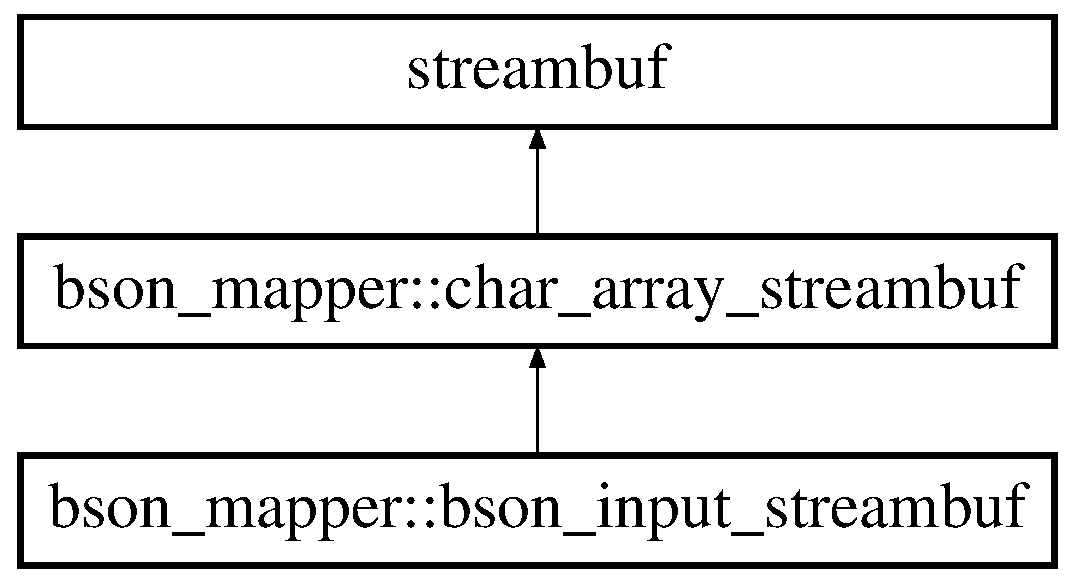
\includegraphics[height=3.000000cm]{classbson__mapper_1_1bson__input__streambuf}
\end{center}
\end{figure}
\subsection*{Additional Inherited Members}


\subsection{Detailed Description}
A wrapper from \hyperlink{classbson__mapper_1_1char__array__streambuf}{char\+\_\+array\+\_\+streambuf}, that uses the data from a B\+S\+ON document view as a buffer. 

The documentation for this class was generated from the following file\+:\begin{DoxyCompactItemize}
\item 
src/bson\+\_\+mapper/bson\+\_\+streambuf.\+hpp\end{DoxyCompactItemize}

\hypertarget{classbson__mapper_1_1bson__istream}{}\section{bson\+\_\+mapper\+:\+:bson\+\_\+istream Class Reference}
\label{classbson__mapper_1_1bson__istream}\index{bson\+\_\+mapper\+::bson\+\_\+istream@{bson\+\_\+mapper\+::bson\+\_\+istream}}


An istream that uses a B\+S\+ON document as a buffer.  




{\ttfamily \#include $<$bson\+\_\+streambuf.\+hpp$>$}

Inheritance diagram for bson\+\_\+mapper\+:\+:bson\+\_\+istream\+:\begin{figure}[H]
\begin{center}
\leavevmode
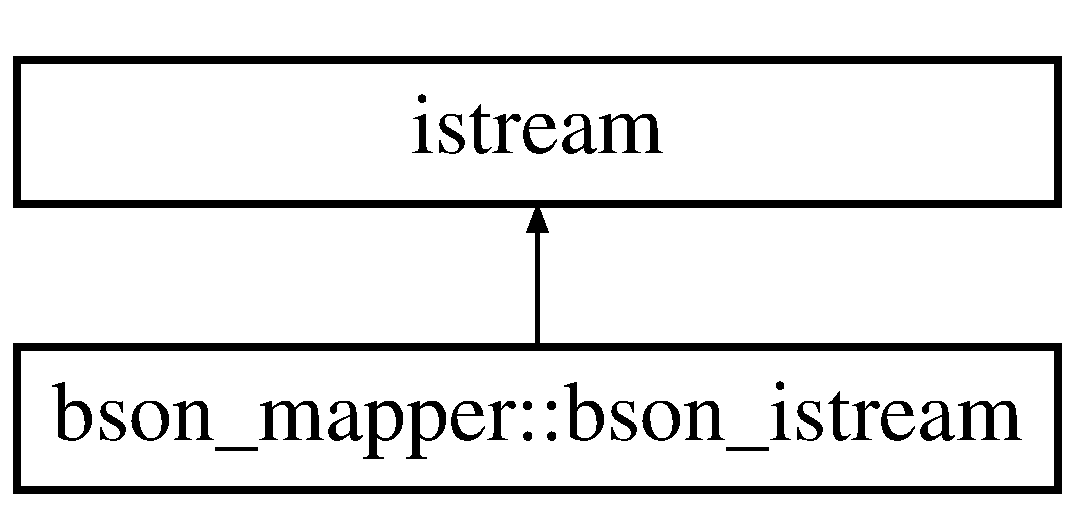
\includegraphics[height=2.000000cm]{classbson__mapper_1_1bson__istream}
\end{center}
\end{figure}


\subsection{Detailed Description}
An istream that uses a B\+S\+ON document as a buffer. 

While objects of this class do not own the underlying buffer, they do own the streambuf object associated with it.

By default, istream objects do not delete their streambuffers when they are destroyed, so this class allows one to create a stream without dealing with the underlying streambuf object. 

The documentation for this class was generated from the following file\+:\begin{DoxyCompactItemize}
\item 
src/bson\+\_\+mapper/bson\+\_\+streambuf.\+hpp\end{DoxyCompactItemize}

\hypertarget{classbson__mapper_1_1bson__ostream}{}\section{bson\+\_\+mapper\+:\+:bson\+\_\+ostream Class Reference}
\label{classbson__mapper_1_1bson__ostream}\index{bson\+\_\+mapper\+::bson\+\_\+ostream@{bson\+\_\+mapper\+::bson\+\_\+ostream}}


An ostream that writes bytes of B\+S\+ON documents into a collection.  




{\ttfamily \#include $<$bson\+\_\+streambuf.\+hpp$>$}

Inheritance diagram for bson\+\_\+mapper\+:\+:bson\+\_\+ostream\+:\begin{figure}[H]
\begin{center}
\leavevmode
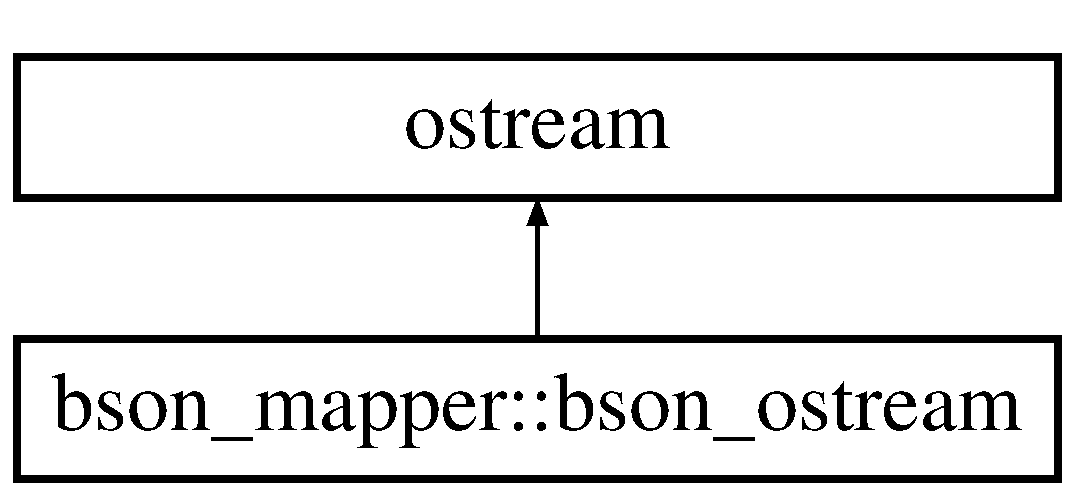
\includegraphics[height=2.000000cm]{classbson__mapper_1_1bson__ostream}
\end{center}
\end{figure}


\subsection{Detailed Description}
An ostream that writes bytes of B\+S\+ON documents into a collection. 

The stream owns its own \hyperlink{classbson__mapper_1_1bson__output__streambuf}{bson\+\_\+output\+\_\+streambuf} object, making creation and management of such streams easier. 

The documentation for this class was generated from the following file\+:\begin{DoxyCompactItemize}
\item 
src/bson\+\_\+mapper/bson\+\_\+streambuf.\+hpp\end{DoxyCompactItemize}

\hypertarget{classbson__mapper_1_1bson__output__streambuf}{}\section{bson\+\_\+mapper\+:\+:bson\+\_\+output\+\_\+streambuf Class Reference}
\label{classbson__mapper_1_1bson__output__streambuf}\index{bson\+\_\+mapper\+::bson\+\_\+output\+\_\+streambuf@{bson\+\_\+mapper\+::bson\+\_\+output\+\_\+streambuf}}


A streambuffer that accepts one or more B\+S\+ON documents as bytes of B\+S\+ON data.  




{\ttfamily \#include $<$bson\+\_\+streambuf.\+hpp$>$}

Inheritance diagram for bson\+\_\+mapper\+:\+:bson\+\_\+output\+\_\+streambuf\+:\begin{figure}[H]
\begin{center}
\leavevmode
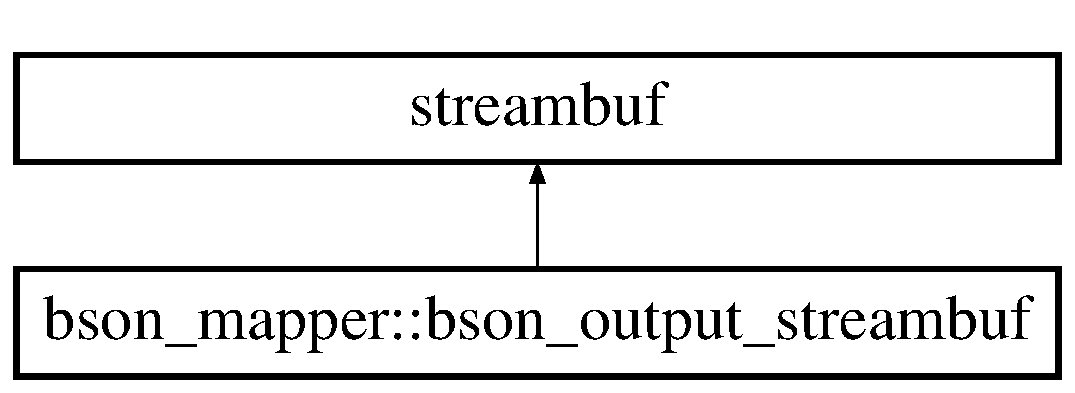
\includegraphics[height=2.000000cm]{classbson__mapper_1_1bson__output__streambuf}
\end{center}
\end{figure}
\subsection*{Public Member Functions}
\begin{DoxyCompactItemize}
\item 
\hyperlink{classbson__mapper_1_1bson__output__streambuf_afbbff25db476b5ec8c166a030664579a}{bson\+\_\+output\+\_\+streambuf} (document\+\_\+callback cb)
\begin{DoxyCompactList}\small\item\em Constructs a new B\+S\+ON Output Streambuffer that passes documents to the given callback function. \end{DoxyCompactList}\item 
int \hyperlink{classbson__mapper_1_1bson__output__streambuf_aebf518d6dd7cad563dced7299b05456e}{overflow} (int ch) override
\begin{DoxyCompactList}\small\item\em This function is called when writing to the stream and the buffer is full. \end{DoxyCompactList}\item 
virtual int \hyperlink{classbson__mapper_1_1bson__output__streambuf_abf1753938d33b31f2408967589ca64ee}{underflow} () override
\begin{DoxyCompactList}\small\item\em This function always returns E\+OF, since one should not write from an output stream. \end{DoxyCompactList}\end{DoxyCompactItemize}


\subsection{Detailed Description}
A streambuffer that accepts one or more B\+S\+ON documents as bytes of B\+S\+ON data. 

When a document is complete, it is passed into the user-\/provided callback. N\+O\+TE\+: This does not perform any validation on the B\+S\+ON files, and simply uses their first four bytes to judge the document length. 

\subsection{Constructor \& Destructor Documentation}
\index{bson\+\_\+mapper\+::bson\+\_\+output\+\_\+streambuf@{bson\+\_\+mapper\+::bson\+\_\+output\+\_\+streambuf}!bson\+\_\+output\+\_\+streambuf@{bson\+\_\+output\+\_\+streambuf}}
\index{bson\+\_\+output\+\_\+streambuf@{bson\+\_\+output\+\_\+streambuf}!bson\+\_\+mapper\+::bson\+\_\+output\+\_\+streambuf@{bson\+\_\+mapper\+::bson\+\_\+output\+\_\+streambuf}}
\subsubsection[{\texorpdfstring{bson\+\_\+output\+\_\+streambuf(document\+\_\+callback cb)}{bson_output_streambuf(document_callback cb)}}]{\setlength{\rightskip}{0pt plus 5cm}bson\+\_\+mapper\+::bson\+\_\+output\+\_\+streambuf\+::bson\+\_\+output\+\_\+streambuf (
\begin{DoxyParamCaption}
\item[{document\+\_\+callback}]{cb}
\end{DoxyParamCaption}
)}\hypertarget{classbson__mapper_1_1bson__output__streambuf_afbbff25db476b5ec8c166a030664579a}{}\label{classbson__mapper_1_1bson__output__streambuf_afbbff25db476b5ec8c166a030664579a}


Constructs a new B\+S\+ON Output Streambuffer that passes documents to the given callback function. 


\begin{DoxyParams}{Parameters}
{\em cb} & A function that takes a document\+::value and returns void. \\
\hline
\end{DoxyParams}


\subsection{Member Function Documentation}
\index{bson\+\_\+mapper\+::bson\+\_\+output\+\_\+streambuf@{bson\+\_\+mapper\+::bson\+\_\+output\+\_\+streambuf}!overflow@{overflow}}
\index{overflow@{overflow}!bson\+\_\+mapper\+::bson\+\_\+output\+\_\+streambuf@{bson\+\_\+mapper\+::bson\+\_\+output\+\_\+streambuf}}
\subsubsection[{\texorpdfstring{overflow(int ch) override}{overflow(int ch) override}}]{\setlength{\rightskip}{0pt plus 5cm}int bson\+\_\+mapper\+::bson\+\_\+output\+\_\+streambuf\+::overflow (
\begin{DoxyParamCaption}
\item[{int}]{ch}
\end{DoxyParamCaption}
)\hspace{0.3cm}{\ttfamily [override]}}\hypertarget{classbson__mapper_1_1bson__output__streambuf_aebf518d6dd7cad563dced7299b05456e}{}\label{classbson__mapper_1_1bson__output__streambuf_aebf518d6dd7cad563dced7299b05456e}


This function is called when writing to the stream and the buffer is full. 

Since we don\textquotesingle{}t define a buffer, this is called with every character. 
\begin{DoxyParams}{Parameters}
{\em ch} & The byte of B\+S\+ON to insert. \\
\hline
\end{DoxyParams}
\begin{DoxyReturn}{Returns}
The inserted byte, or E\+OF if something failed. 
\end{DoxyReturn}
\index{bson\+\_\+mapper\+::bson\+\_\+output\+\_\+streambuf@{bson\+\_\+mapper\+::bson\+\_\+output\+\_\+streambuf}!underflow@{underflow}}
\index{underflow@{underflow}!bson\+\_\+mapper\+::bson\+\_\+output\+\_\+streambuf@{bson\+\_\+mapper\+::bson\+\_\+output\+\_\+streambuf}}
\subsubsection[{\texorpdfstring{underflow() override}{underflow() override}}]{\setlength{\rightskip}{0pt plus 5cm}virtual int bson\+\_\+mapper\+::bson\+\_\+output\+\_\+streambuf\+::underflow (
\begin{DoxyParamCaption}
{}
\end{DoxyParamCaption}
)\hspace{0.3cm}{\ttfamily [override]}, {\ttfamily [virtual]}}\hypertarget{classbson__mapper_1_1bson__output__streambuf_abf1753938d33b31f2408967589ca64ee}{}\label{classbson__mapper_1_1bson__output__streambuf_abf1753938d33b31f2408967589ca64ee}


This function always returns E\+OF, since one should not write from an output stream. 

\begin{DoxyReturn}{Returns}
E\+OF 
\end{DoxyReturn}


The documentation for this class was generated from the following file\+:\begin{DoxyCompactItemize}
\item 
src/bson\+\_\+mapper/bson\+\_\+streambuf.\+hpp\end{DoxyCompactItemize}

\hypertarget{classbson__mapper_1_1BSONInputArchive}{}\section{bson\+\_\+mapper\+:\+:B\+S\+O\+N\+Input\+Archive Class Reference}
\label{classbson__mapper_1_1BSONInputArchive}\index{bson\+\_\+mapper\+::\+B\+S\+O\+N\+Input\+Archive@{bson\+\_\+mapper\+::\+B\+S\+O\+N\+Input\+Archive}}
Inheritance diagram for bson\+\_\+mapper\+:\+:B\+S\+O\+N\+Input\+Archive\+:\begin{figure}[H]
\begin{center}
\leavevmode
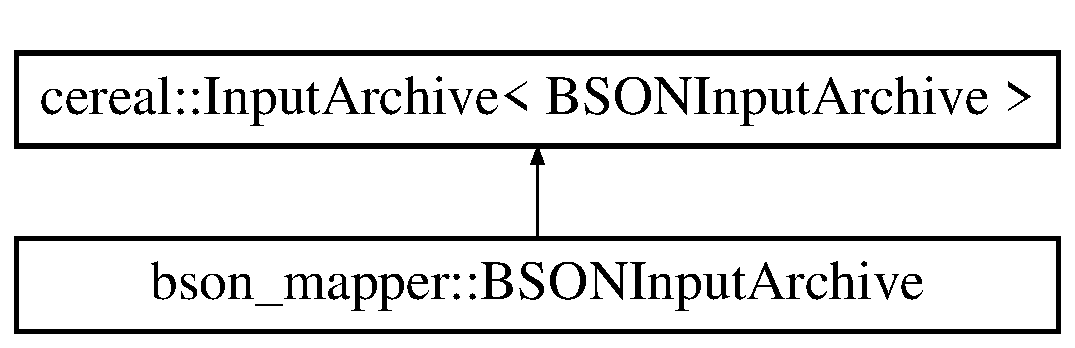
\includegraphics[height=2.000000cm]{classbson__mapper_1_1BSONInputArchive}
\end{center}
\end{figure}
\subsection*{Public Member Functions}
\begin{DoxyCompactItemize}
\item 
\hyperlink{classbson__mapper_1_1BSONInputArchive_a6b8ddbbd18800ef0f8e250c31da095e8}{B\+S\+O\+N\+Input\+Archive} (std\+::istream \&stream)
\begin{DoxyCompactList}\small\item\em Construct a \hyperlink{classbson__mapper_1_1BSONInputArchive}{B\+S\+O\+N\+Input\+Archive} from an input stream of B\+S\+ON data. \end{DoxyCompactList}\item 
bool \hyperlink{classbson__mapper_1_1BSONInputArchive_a0b8d043db14caa7d4e35d8e5300cd69f}{will\+Search\+Yield\+Value} ()
\begin{DoxyCompactList}\small\item\em Checks if the next invocation of search() will yield a value. \end{DoxyCompactList}\item 
bool \hyperlink{classbson__mapper_1_1BSONInputArchive_ab0b224d34f6dd2fd9ee542571536638b}{start\+Root\+Element\+If\+Root} ()
\begin{DoxyCompactList}\small\item\em Pushes a root element on the node stack if we\textquotesingle{}re in root. \end{DoxyCompactList}\item 
void \hyperlink{classbson__mapper_1_1BSONInputArchive_a1100f99901973ebefab2198d2381e953}{finish\+Root\+Element\+If\+Root\+Element} ()\hypertarget{classbson__mapper_1_1BSONInputArchive_a1100f99901973ebefab2198d2381e953}{}\label{classbson__mapper_1_1BSONInputArchive_a1100f99901973ebefab2198d2381e953}

\begin{DoxyCompactList}\small\item\em Pops the node stack and iterates to the next B\+S\+ON view if the top of the stack specifies that we are in a root element. \end{DoxyCompactList}\item 
void \hyperlink{classbson__mapper_1_1BSONInputArchive_a6f74b53f0989e9222be00dec0e6d350f}{start\+Node} ()\hypertarget{classbson__mapper_1_1BSONInputArchive_a6f74b53f0989e9222be00dec0e6d350f}{}\label{classbson__mapper_1_1BSONInputArchive_a6f74b53f0989e9222be00dec0e6d350f}

\begin{DoxyCompactList}\small\item\em Starts a new node, and update the stacks so that we fetch the correct data when calling search(). \end{DoxyCompactList}\item 
void \hyperlink{classbson__mapper_1_1BSONInputArchive_a9360961eba7c7c430329eed30667a2de}{finish\+Node} ()\hypertarget{classbson__mapper_1_1BSONInputArchive_a9360961eba7c7c430329eed30667a2de}{}\label{classbson__mapper_1_1BSONInputArchive_a9360961eba7c7c430329eed30667a2de}

\begin{DoxyCompactList}\small\item\em Finishes the most recently started node by popping relevant stacks and, if necessary, iterating to the next root B\+S\+ON document. \end{DoxyCompactList}\item 
void \hyperlink{classbson__mapper_1_1BSONInputArchive_a5536f703a1f8d0f19fca666290ee6b42}{set\+Next\+Name} (const char $\ast$name)
\begin{DoxyCompactList}\small\item\em Sets the name for the next node created with start\+Node. \end{DoxyCompactList}\item 
void \hyperlink{classbson__mapper_1_1BSONInputArchive_a457680690d03b26a9600b9139d1b9bd9}{load\+Value} (std\+::chrono\+::system\+\_\+clock\+::time\+\_\+point \&val)
\begin{DoxyCompactList}\small\item\em Loads a B\+S\+ON datetime from the current node and puts it into a std\+::chrono\+::system\+\_\+clock\+::time\+\_\+point. \end{DoxyCompactList}\item 
void \hyperlink{classbson__mapper_1_1BSONInputArchive_afa63fee8fca6808c51178fb6a7767abd}{load\+Value} (std\+::string \&val)
\begin{DoxyCompactList}\small\item\em Loads a B\+S\+ON U\+T\+F-\/8 value from the current node and puts it into a std\+::string. \end{DoxyCompactList}\item 
void \hyperlink{classbson__mapper_1_1BSONInputArchive_a28c16081fe45749c56f5d65b1ab01d40}{load\+Size} (cereal\+::size\+\_\+type \&size)
\begin{DoxyCompactList}\small\item\em Loads the size for a Size\+Tag, which is used by Cereal to determine how many elements to put into a container such as a std\+::vector. \end{DoxyCompactList}\item 
void \hyperlink{classbson__mapper_1_1BSONInputArchive_ad3fae22817ce463e8a3055a1f04e7a91}{load\+Underlying\+Data\+For\+Current\+Node} (\hyperlink{classbson__mapper_1_1UnderlyingBSONDataBase}{Underlying\+B\+S\+O\+N\+Data\+Base} \&underlying\+Data)\hypertarget{classbson__mapper_1_1BSONInputArchive_ad3fae22817ce463e8a3055a1f04e7a91}{}\label{classbson__mapper_1_1BSONInputArchive_ad3fae22817ce463e8a3055a1f04e7a91}

\begin{DoxyCompactList}\small\item\em Returns a shared pointer to the underlying data of the current node, loading the size in bytes in a size\+\_\+t reference argument. \end{DoxyCompactList}\end{DoxyCompactItemize}


\subsection{Constructor \& Destructor Documentation}
\index{bson\+\_\+mapper\+::\+B\+S\+O\+N\+Input\+Archive@{bson\+\_\+mapper\+::\+B\+S\+O\+N\+Input\+Archive}!B\+S\+O\+N\+Input\+Archive@{B\+S\+O\+N\+Input\+Archive}}
\index{B\+S\+O\+N\+Input\+Archive@{B\+S\+O\+N\+Input\+Archive}!bson\+\_\+mapper\+::\+B\+S\+O\+N\+Input\+Archive@{bson\+\_\+mapper\+::\+B\+S\+O\+N\+Input\+Archive}}
\subsubsection[{\texorpdfstring{B\+S\+O\+N\+Input\+Archive(std\+::istream \&stream)}{BSONInputArchive(std::istream &stream)}}]{\setlength{\rightskip}{0pt plus 5cm}bson\+\_\+mapper\+::\+B\+S\+O\+N\+Input\+Archive\+::\+B\+S\+O\+N\+Input\+Archive (
\begin{DoxyParamCaption}
\item[{std\+::istream \&}]{stream}
\end{DoxyParamCaption}
)\hspace{0.3cm}{\ttfamily [inline]}}\hypertarget{classbson__mapper_1_1BSONInputArchive_a6b8ddbbd18800ef0f8e250c31da095e8}{}\label{classbson__mapper_1_1BSONInputArchive_a6b8ddbbd18800ef0f8e250c31da095e8}


Construct a \hyperlink{classbson__mapper_1_1BSONInputArchive}{B\+S\+O\+N\+Input\+Archive} from an input stream of B\+S\+ON data. 


\begin{DoxyParams}{Parameters}
{\em stream} & The stream from which to read B\+S\+ON data. \\
\hline
\end{DoxyParams}


\subsection{Member Function Documentation}
\index{bson\+\_\+mapper\+::\+B\+S\+O\+N\+Input\+Archive@{bson\+\_\+mapper\+::\+B\+S\+O\+N\+Input\+Archive}!load\+Size@{load\+Size}}
\index{load\+Size@{load\+Size}!bson\+\_\+mapper\+::\+B\+S\+O\+N\+Input\+Archive@{bson\+\_\+mapper\+::\+B\+S\+O\+N\+Input\+Archive}}
\subsubsection[{\texorpdfstring{load\+Size(cereal\+::size\+\_\+type \&size)}{loadSize(cereal::size_type &size)}}]{\setlength{\rightskip}{0pt plus 5cm}void bson\+\_\+mapper\+::\+B\+S\+O\+N\+Input\+Archive\+::load\+Size (
\begin{DoxyParamCaption}
\item[{cereal\+::size\+\_\+type \&}]{size}
\end{DoxyParamCaption}
)\hspace{0.3cm}{\ttfamily [inline]}}\hypertarget{classbson__mapper_1_1BSONInputArchive_a28c16081fe45749c56f5d65b1ab01d40}{}\label{classbson__mapper_1_1BSONInputArchive_a28c16081fe45749c56f5d65b1ab01d40}


Loads the size for a Size\+Tag, which is used by Cereal to determine how many elements to put into a container such as a std\+::vector. 


\begin{DoxyParams}{Parameters}
{\em size} & A reference to the size value that will be set to the size of the array at the top of the stack. \\
\hline
\end{DoxyParams}
\index{bson\+\_\+mapper\+::\+B\+S\+O\+N\+Input\+Archive@{bson\+\_\+mapper\+::\+B\+S\+O\+N\+Input\+Archive}!load\+Value@{load\+Value}}
\index{load\+Value@{load\+Value}!bson\+\_\+mapper\+::\+B\+S\+O\+N\+Input\+Archive@{bson\+\_\+mapper\+::\+B\+S\+O\+N\+Input\+Archive}}
\subsubsection[{\texorpdfstring{load\+Value(std\+::chrono\+::system\+\_\+clock\+::time\+\_\+point \&val)}{loadValue(std::chrono::system_clock::time_point &val)}}]{\setlength{\rightskip}{0pt plus 5cm}void bson\+\_\+mapper\+::\+B\+S\+O\+N\+Input\+Archive\+::load\+Value (
\begin{DoxyParamCaption}
\item[{std\+::chrono\+::system\+\_\+clock\+::time\+\_\+point \&}]{val}
\end{DoxyParamCaption}
)\hspace{0.3cm}{\ttfamily [inline]}}\hypertarget{classbson__mapper_1_1BSONInputArchive_a457680690d03b26a9600b9139d1b9bd9}{}\label{classbson__mapper_1_1BSONInputArchive_a457680690d03b26a9600b9139d1b9bd9}


Loads a B\+S\+ON datetime from the current node and puts it into a std\+::chrono\+::system\+\_\+clock\+::time\+\_\+point. 


\begin{DoxyParams}{Parameters}
{\em val} & The time\+\_\+point variable into which the datetime will be loaded. \\
\hline
\end{DoxyParams}
\index{bson\+\_\+mapper\+::\+B\+S\+O\+N\+Input\+Archive@{bson\+\_\+mapper\+::\+B\+S\+O\+N\+Input\+Archive}!load\+Value@{load\+Value}}
\index{load\+Value@{load\+Value}!bson\+\_\+mapper\+::\+B\+S\+O\+N\+Input\+Archive@{bson\+\_\+mapper\+::\+B\+S\+O\+N\+Input\+Archive}}
\subsubsection[{\texorpdfstring{load\+Value(std\+::string \&val)}{loadValue(std::string &val)}}]{\setlength{\rightskip}{0pt plus 5cm}void bson\+\_\+mapper\+::\+B\+S\+O\+N\+Input\+Archive\+::load\+Value (
\begin{DoxyParamCaption}
\item[{std\+::string \&}]{val}
\end{DoxyParamCaption}
)\hspace{0.3cm}{\ttfamily [inline]}}\hypertarget{classbson__mapper_1_1BSONInputArchive_afa63fee8fca6808c51178fb6a7767abd}{}\label{classbson__mapper_1_1BSONInputArchive_afa63fee8fca6808c51178fb6a7767abd}


Loads a B\+S\+ON U\+T\+F-\/8 value from the current node and puts it into a std\+::string. 


\begin{DoxyParams}{Parameters}
{\em val} & The std\+::string variable into which the U\+T\+F-\/8 will be loaded. \\
\hline
\end{DoxyParams}
\index{bson\+\_\+mapper\+::\+B\+S\+O\+N\+Input\+Archive@{bson\+\_\+mapper\+::\+B\+S\+O\+N\+Input\+Archive}!set\+Next\+Name@{set\+Next\+Name}}
\index{set\+Next\+Name@{set\+Next\+Name}!bson\+\_\+mapper\+::\+B\+S\+O\+N\+Input\+Archive@{bson\+\_\+mapper\+::\+B\+S\+O\+N\+Input\+Archive}}
\subsubsection[{\texorpdfstring{set\+Next\+Name(const char $\ast$name)}{setNextName(const char *name)}}]{\setlength{\rightskip}{0pt plus 5cm}void bson\+\_\+mapper\+::\+B\+S\+O\+N\+Input\+Archive\+::set\+Next\+Name (
\begin{DoxyParamCaption}
\item[{const char $\ast$}]{name}
\end{DoxyParamCaption}
)\hspace{0.3cm}{\ttfamily [inline]}}\hypertarget{classbson__mapper_1_1BSONInputArchive_a5536f703a1f8d0f19fca666290ee6b42}{}\label{classbson__mapper_1_1BSONInputArchive_a5536f703a1f8d0f19fca666290ee6b42}


Sets the name for the next node created with start\+Node. 


\begin{DoxyParams}{Parameters}
{\em name} & The name of the next node \\
\hline
\end{DoxyParams}
\index{bson\+\_\+mapper\+::\+B\+S\+O\+N\+Input\+Archive@{bson\+\_\+mapper\+::\+B\+S\+O\+N\+Input\+Archive}!start\+Root\+Element\+If\+Root@{start\+Root\+Element\+If\+Root}}
\index{start\+Root\+Element\+If\+Root@{start\+Root\+Element\+If\+Root}!bson\+\_\+mapper\+::\+B\+S\+O\+N\+Input\+Archive@{bson\+\_\+mapper\+::\+B\+S\+O\+N\+Input\+Archive}}
\subsubsection[{\texorpdfstring{start\+Root\+Element\+If\+Root()}{startRootElementIfRoot()}}]{\setlength{\rightskip}{0pt plus 5cm}bool bson\+\_\+mapper\+::\+B\+S\+O\+N\+Input\+Archive\+::start\+Root\+Element\+If\+Root (
\begin{DoxyParamCaption}
{}
\end{DoxyParamCaption}
)\hspace{0.3cm}{\ttfamily [inline]}}\hypertarget{classbson__mapper_1_1BSONInputArchive_ab0b224d34f6dd2fd9ee542571536638b}{}\label{classbson__mapper_1_1BSONInputArchive_ab0b224d34f6dd2fd9ee542571536638b}


Pushes a root element on the node stack if we\textquotesingle{}re in root. 

\begin{DoxyReturn}{Returns}
true if a root element was created, false otherwise. 
\end{DoxyReturn}
\index{bson\+\_\+mapper\+::\+B\+S\+O\+N\+Input\+Archive@{bson\+\_\+mapper\+::\+B\+S\+O\+N\+Input\+Archive}!will\+Search\+Yield\+Value@{will\+Search\+Yield\+Value}}
\index{will\+Search\+Yield\+Value@{will\+Search\+Yield\+Value}!bson\+\_\+mapper\+::\+B\+S\+O\+N\+Input\+Archive@{bson\+\_\+mapper\+::\+B\+S\+O\+N\+Input\+Archive}}
\subsubsection[{\texorpdfstring{will\+Search\+Yield\+Value()}{willSearchYieldValue()}}]{\setlength{\rightskip}{0pt plus 5cm}bool bson\+\_\+mapper\+::\+B\+S\+O\+N\+Input\+Archive\+::will\+Search\+Yield\+Value (
\begin{DoxyParamCaption}
{}
\end{DoxyParamCaption}
)\hspace{0.3cm}{\ttfamily [inline]}}\hypertarget{classbson__mapper_1_1BSONInputArchive_a0b8d043db14caa7d4e35d8e5300cd69f}{}\label{classbson__mapper_1_1BSONInputArchive_a0b8d043db14caa7d4e35d8e5300cd69f}


Checks if the next invocation of search() will yield a value. 

Used to check if a particular optional element, embedded document, or embedded array exists.

If search() would indeed return a value, it is cached here so that the logic in search() will not need to be repeated.

\begin{DoxyReturn}{Returns}
true if the next invocation of search with the current \+\_\+next\+Name yields a value, false otherwise. 
\end{DoxyReturn}


The documentation for this class was generated from the following file\+:\begin{DoxyCompactItemize}
\item 
src/bson\+\_\+mapper/bson\+\_\+archiver.\+hpp\end{DoxyCompactItemize}

\hypertarget{classbson__mapper_1_1BSONOutputArchive}{}\section{bson\+\_\+mapper\+:\+:B\+S\+O\+N\+Output\+Archive Class Reference}
\label{classbson__mapper_1_1BSONOutputArchive}\index{bson\+\_\+mapper\+::\+B\+S\+O\+N\+Output\+Archive@{bson\+\_\+mapper\+::\+B\+S\+O\+N\+Output\+Archive}}
Inheritance diagram for bson\+\_\+mapper\+:\+:B\+S\+O\+N\+Output\+Archive\+:\begin{figure}[H]
\begin{center}
\leavevmode
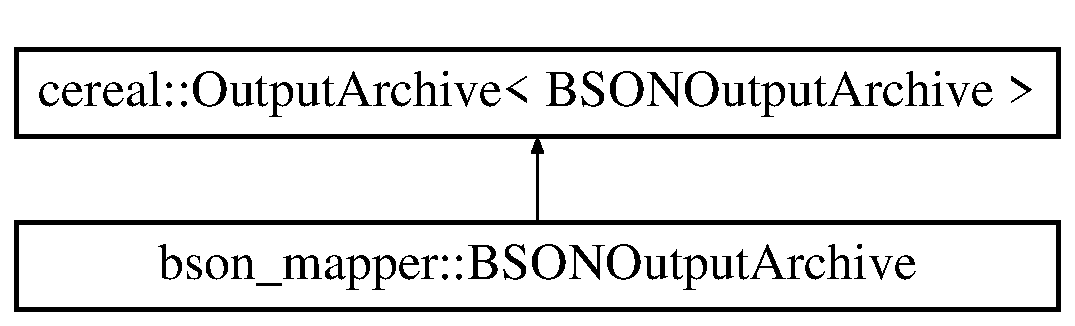
\includegraphics[height=2.000000cm]{classbson__mapper_1_1BSONOutputArchive}
\end{center}
\end{figure}
\subsection*{Public Member Functions}
\begin{DoxyCompactItemize}
\item 
\hyperlink{classbson__mapper_1_1BSONOutputArchive_a07af9bf8f5a9fa281c6424bfe39f453f}{B\+S\+O\+N\+Output\+Archive} (std\+::ostream \&stream, bool dot\+Notation\+Mode=false)
\begin{DoxyCompactList}\small\item\em Construct a \hyperlink{classbson__mapper_1_1BSONOutputArchive}{B\+S\+O\+N\+Output\+Archive} that will output serialized classes as B\+S\+ON to the provided stream. \end{DoxyCompactList}\end{DoxyCompactItemize}


\subsection{Constructor \& Destructor Documentation}
\index{bson\+\_\+mapper\+::\+B\+S\+O\+N\+Output\+Archive@{bson\+\_\+mapper\+::\+B\+S\+O\+N\+Output\+Archive}!B\+S\+O\+N\+Output\+Archive@{B\+S\+O\+N\+Output\+Archive}}
\index{B\+S\+O\+N\+Output\+Archive@{B\+S\+O\+N\+Output\+Archive}!bson\+\_\+mapper\+::\+B\+S\+O\+N\+Output\+Archive@{bson\+\_\+mapper\+::\+B\+S\+O\+N\+Output\+Archive}}
\subsubsection[{\texorpdfstring{B\+S\+O\+N\+Output\+Archive(std\+::ostream \&stream, bool dot\+Notation\+Mode=false)}{BSONOutputArchive(std::ostream &stream, bool dotNotationMode=false)}}]{\setlength{\rightskip}{0pt plus 5cm}bson\+\_\+mapper\+::\+B\+S\+O\+N\+Output\+Archive\+::\+B\+S\+O\+N\+Output\+Archive (
\begin{DoxyParamCaption}
\item[{std\+::ostream \&}]{stream, }
\item[{bool}]{dot\+Notation\+Mode = {\ttfamily false}}
\end{DoxyParamCaption}
)\hspace{0.3cm}{\ttfamily [inline]}}\hypertarget{classbson__mapper_1_1BSONOutputArchive_a07af9bf8f5a9fa281c6424bfe39f453f}{}\label{classbson__mapper_1_1BSONOutputArchive_a07af9bf8f5a9fa281c6424bfe39f453f}


Construct a \hyperlink{classbson__mapper_1_1BSONOutputArchive}{B\+S\+O\+N\+Output\+Archive} that will output serialized classes as B\+S\+ON to the provided stream. 


\begin{DoxyParams}{Parameters}
{\em stream} & The stream to which the archiver will output B\+S\+ON data.\\
\hline
{\em dot\+Notation\+Mode} & If set to true, the \hyperlink{classbson__mapper_1_1BSONOutputArchive}{B\+S\+O\+N\+Output\+Archive} will output the values in embedded documents in dot notation. This is useful when specifying the arguments to a \$set field in a Mongo\+DB update command.\\
\hline
\end{DoxyParams}
\begin{DoxySeeAlso}{See also}
\href{https://docs.mongodb.com/manual/core/document/#embedded-documents}{\tt https\+://docs.\+mongodb.\+com/manual/core/document/\#embedded-\/documents}
\end{DoxySeeAlso}
\begin{DoxyWarning}{Warning}
Documents produced by the archiver in dot\+Notation\+Mode are not compatible with the B\+S\+O\+N\+Input\+Archiver and are only intended to be used as a way to produce the argument to \$set. 
\end{DoxyWarning}


The documentation for this class was generated from the following file\+:\begin{DoxyCompactItemize}
\item 
src/bson\+\_\+mapper/bson\+\_\+archiver.\+hpp\end{DoxyCompactItemize}

\hypertarget{classbson__mapper_1_1char__array__streambuf}{}\section{bson\+\_\+mapper\+:\+:char\+\_\+array\+\_\+streambuf Class Reference}
\label{classbson__mapper_1_1char__array__streambuf}\index{bson\+\_\+mapper\+::char\+\_\+array\+\_\+streambuf@{bson\+\_\+mapper\+::char\+\_\+array\+\_\+streambuf}}


An input streambuf that uses an existing byte array as a buffer.  




{\ttfamily \#include $<$bson\+\_\+streambuf.\+hpp$>$}

Inheritance diagram for bson\+\_\+mapper\+:\+:char\+\_\+array\+\_\+streambuf\+:\begin{figure}[H]
\begin{center}
\leavevmode
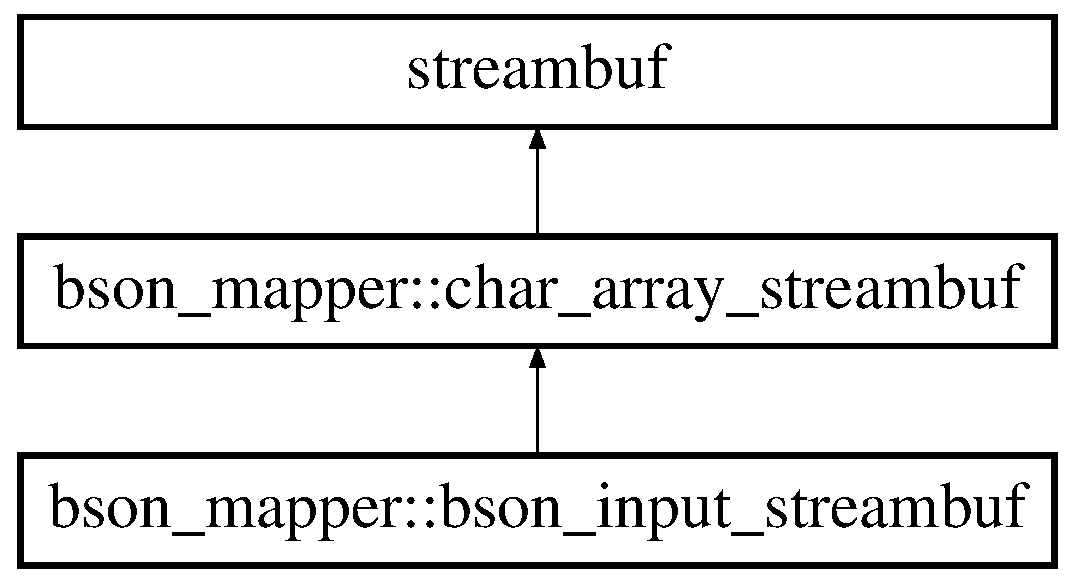
\includegraphics[height=3.000000cm]{classbson__mapper_1_1char__array__streambuf}
\end{center}
\end{figure}
\subsection*{Public Member Functions}
\begin{DoxyCompactItemize}
\item 
\hyperlink{classbson__mapper_1_1char__array__streambuf_a5cba6b0b5b8fab77b956375b4f8f9355}{char\+\_\+array\+\_\+streambuf} (const char $\ast$data, size\+\_\+t len)
\begin{DoxyCompactList}\small\item\em Create a streambuf around the given byte array. \end{DoxyCompactList}\end{DoxyCompactItemize}


\subsection{Detailed Description}
An input streambuf that uses an existing byte array as a buffer. 

\subsection{Constructor \& Destructor Documentation}
\index{bson\+\_\+mapper\+::char\+\_\+array\+\_\+streambuf@{bson\+\_\+mapper\+::char\+\_\+array\+\_\+streambuf}!char\+\_\+array\+\_\+streambuf@{char\+\_\+array\+\_\+streambuf}}
\index{char\+\_\+array\+\_\+streambuf@{char\+\_\+array\+\_\+streambuf}!bson\+\_\+mapper\+::char\+\_\+array\+\_\+streambuf@{bson\+\_\+mapper\+::char\+\_\+array\+\_\+streambuf}}
\subsubsection[{\texorpdfstring{char\+\_\+array\+\_\+streambuf(const char $\ast$data, size\+\_\+t len)}{char_array_streambuf(const char *data, size_t len)}}]{\setlength{\rightskip}{0pt plus 5cm}bson\+\_\+mapper\+::char\+\_\+array\+\_\+streambuf\+::char\+\_\+array\+\_\+streambuf (
\begin{DoxyParamCaption}
\item[{const char $\ast$}]{data, }
\item[{size\+\_\+t}]{len}
\end{DoxyParamCaption}
)}\hypertarget{classbson__mapper_1_1char__array__streambuf_a5cba6b0b5b8fab77b956375b4f8f9355}{}\label{classbson__mapper_1_1char__array__streambuf_a5cba6b0b5b8fab77b956375b4f8f9355}


Create a streambuf around the given byte array. 

The caller is responsible for maintaining the lifetime of the underlying data. 
\begin{DoxyParams}{Parameters}
{\em data} & A pointer to the data to be read \\
\hline
{\em len} & The length of the data \\
\hline
\end{DoxyParams}


The documentation for this class was generated from the following file\+:\begin{DoxyCompactItemize}
\item 
src/bson\+\_\+mapper/bson\+\_\+streambuf.\+hpp\end{DoxyCompactItemize}

\hypertarget{classmongo__odm_1_1ComparisonExpr}{}\section{mongo\+\_\+odm\+:\+:Comparison\+Expr$<$ Base, T $>$ Class Template Reference}
\label{classmongo__odm_1_1ComparisonExpr}\index{mongo\+\_\+odm\+::\+Comparison\+Expr$<$ Base, T $>$@{mongo\+\_\+odm\+::\+Comparison\+Expr$<$ Base, T $>$}}


Represents a binary comparison expression between a key and a value.  




{\ttfamily \#include $<$query\+\_\+builder.\+hpp$>$}

\subsection*{Public Member Functions}
\begin{DoxyCompactItemize}
\item 
constexpr \hyperlink{classmongo__odm_1_1ComparisonExpr_a00cedfa66e6c8622149739dffde2e23e}{Comparison\+Expr} (const \hyperlink{structmongo__odm_1_1Nvp}{Nvp}$<$ Base, T $>$ \&nvp, T field, const char $\ast$selector\+\_\+type)
\begin{DoxyCompactList}\small\item\em Constructs a query expression for the given key, value, and comparison type. \end{DoxyCompactList}\item 
void \hyperlink{classmongo__odm_1_1ComparisonExpr_afcfc49aa8b1a0d024fe8a8c0d2441e40}{append\+\_\+to\+\_\+bson} (bsoncxx\+::builder\+::core \&builder) const 
\begin{DoxyCompactList}\small\item\em Appends this expression to a B\+S\+ON core builder, as a key-\/value pair of the form \char`\"{}key\+: \{\$cmp\+: val\}\char`\"{}, where \$cmp is some comparison operator. \end{DoxyCompactList}\item 
\hyperlink{classmongo__odm_1_1ComparisonExpr_a8174f54d033e934b141b3a9ef4480a84}{operator bsoncxx\+::document\+::view\+\_\+or\+\_\+value} () const 
\begin{DoxyCompactList}\small\item\em Converts the expression to a B\+S\+ON filter for a query. \end{DoxyCompactList}\end{DoxyCompactItemize}


\subsection{Detailed Description}
\subsubsection*{template$<$typename Base, typename T$>$\\*
class mongo\+\_\+odm\+::\+Comparison\+Expr$<$ Base, T $>$}

Represents a binary comparison expression between a key and a value. 

e.\+g. (User.\+age $>$ 21). 

\subsection{Constructor \& Destructor Documentation}
\index{mongo\+\_\+odm\+::\+Comparison\+Expr@{mongo\+\_\+odm\+::\+Comparison\+Expr}!Comparison\+Expr@{Comparison\+Expr}}
\index{Comparison\+Expr@{Comparison\+Expr}!mongo\+\_\+odm\+::\+Comparison\+Expr@{mongo\+\_\+odm\+::\+Comparison\+Expr}}
\subsubsection[{\texorpdfstring{Comparison\+Expr(const Nvp$<$ Base, T $>$ \&nvp, T field, const char $\ast$selector\+\_\+type)}{ComparisonExpr(const Nvp< Base, T > &nvp, T field, const char *selector_type)}}]{\setlength{\rightskip}{0pt plus 5cm}template$<$typename Base, typename T$>$ constexpr {\bf mongo\+\_\+odm\+::\+Comparison\+Expr}$<$ Base, T $>$\+::{\bf Comparison\+Expr} (
\begin{DoxyParamCaption}
\item[{const {\bf Nvp}$<$ Base, T $>$ \&}]{nvp, }
\item[{T}]{field, }
\item[{const char $\ast$}]{selector\+\_\+type}
\end{DoxyParamCaption}
)\hspace{0.3cm}{\ttfamily [inline]}}\hypertarget{classmongo__odm_1_1ComparisonExpr_a00cedfa66e6c8622149739dffde2e23e}{}\label{classmongo__odm_1_1ComparisonExpr_a00cedfa66e6c8622149739dffde2e23e}


Constructs a query expression for the given key, value, and comparison type. 


\begin{DoxyParams}{Parameters}
{\em nvp} & A name-\/value pair corresponding to a key in a document \\
\hline
{\em field} & The value that the key is being compared to. \\
\hline
{\em selector\+\_\+type} & The type of comparison operator, such at gt ($>$) or ne (!=). \\
\hline
\end{DoxyParams}


\subsection{Member Function Documentation}
\index{mongo\+\_\+odm\+::\+Comparison\+Expr@{mongo\+\_\+odm\+::\+Comparison\+Expr}!append\+\_\+to\+\_\+bson@{append\+\_\+to\+\_\+bson}}
\index{append\+\_\+to\+\_\+bson@{append\+\_\+to\+\_\+bson}!mongo\+\_\+odm\+::\+Comparison\+Expr@{mongo\+\_\+odm\+::\+Comparison\+Expr}}
\subsubsection[{\texorpdfstring{append\+\_\+to\+\_\+bson(bsoncxx\+::builder\+::core \&builder) const }{append_to_bson(bsoncxx::builder::core &builder) const }}]{\setlength{\rightskip}{0pt plus 5cm}template$<$typename Base, typename T$>$ void {\bf mongo\+\_\+odm\+::\+Comparison\+Expr}$<$ Base, T $>$\+::append\+\_\+to\+\_\+bson (
\begin{DoxyParamCaption}
\item[{bsoncxx\+::builder\+::core \&}]{builder}
\end{DoxyParamCaption}
) const\hspace{0.3cm}{\ttfamily [inline]}}\hypertarget{classmongo__odm_1_1ComparisonExpr_afcfc49aa8b1a0d024fe8a8c0d2441e40}{}\label{classmongo__odm_1_1ComparisonExpr_afcfc49aa8b1a0d024fe8a8c0d2441e40}


Appends this expression to a B\+S\+ON core builder, as a key-\/value pair of the form \char`\"{}key\+: \{\$cmp\+: val\}\char`\"{}, where \$cmp is some comparison operator. 


\begin{DoxyParams}{Parameters}
{\em builder} & A B\+S\+ON core builder \\
\hline
\end{DoxyParams}
\index{mongo\+\_\+odm\+::\+Comparison\+Expr@{mongo\+\_\+odm\+::\+Comparison\+Expr}!operator bsoncxx\+::document\+::view\+\_\+or\+\_\+value@{operator bsoncxx\+::document\+::view\+\_\+or\+\_\+value}}
\index{operator bsoncxx\+::document\+::view\+\_\+or\+\_\+value@{operator bsoncxx\+::document\+::view\+\_\+or\+\_\+value}!mongo\+\_\+odm\+::\+Comparison\+Expr@{mongo\+\_\+odm\+::\+Comparison\+Expr}}
\subsubsection[{\texorpdfstring{operator bsoncxx\+::document\+::view\+\_\+or\+\_\+value() const }{operator bsoncxx::document::view_or_value() const }}]{\setlength{\rightskip}{0pt plus 5cm}template$<$typename Base, typename T$>$ {\bf mongo\+\_\+odm\+::\+Comparison\+Expr}$<$ Base, T $>$\+::operator bsoncxx\+::document\+::view\+\_\+or\+\_\+value (
\begin{DoxyParamCaption}
{}
\end{DoxyParamCaption}
) const\hspace{0.3cm}{\ttfamily [inline]}}\hypertarget{classmongo__odm_1_1ComparisonExpr_a8174f54d033e934b141b3a9ef4480a84}{}\label{classmongo__odm_1_1ComparisonExpr_a8174f54d033e934b141b3a9ef4480a84}


Converts the expression to a B\+S\+ON filter for a query. 

The resulting B\+S\+ON is of the form \char`\"{}\{key\+: \{\$cmp\+: val\}\}\char`\"{}. 

The documentation for this class was generated from the following file\+:\begin{DoxyCompactItemize}
\item 
src/mongo\+\_\+odm/query\+\_\+builder.\+hpp\end{DoxyCompactItemize}

\hypertarget{classmongo__odm_1_1deserializing__cursor}{}\section{mongo\+\_\+odm\+:\+:deserializing\+\_\+cursor$<$ T $>$ Class Template Reference}
\label{classmongo__odm_1_1deserializing__cursor}\index{mongo\+\_\+odm\+::deserializing\+\_\+cursor$<$ T $>$@{mongo\+\_\+odm\+::deserializing\+\_\+cursor$<$ T $>$}}


A class that wraps a mongocxx\+::cursor.  




{\ttfamily \#include $<$deserializing\+\_\+cursor.\+hpp$>$}

\subsection*{Classes}
\begin{DoxyCompactItemize}
\item 
class \hyperlink{classmongo__odm_1_1deserializing__cursor_1_1iterator}{iterator}
\end{DoxyCompactItemize}


\subsection{Detailed Description}
\subsubsection*{template$<$class T$>$\\*
class mongo\+\_\+odm\+::deserializing\+\_\+cursor$<$ T $>$}

A class that wraps a mongocxx\+::cursor. 

It provides an iterator that deserializes the documents yielded by the underlying mongocxx cursor. N\+O\+TE\+: This iterator will skip documents that fail to be deserialized, e.\+g. due to non-\/matching schemas. 

The documentation for this class was generated from the following file\+:\begin{DoxyCompactItemize}
\item 
src/mongo\+\_\+odm/deserializing\+\_\+cursor.\+hpp\end{DoxyCompactItemize}

\hypertarget{structbson__mapper_1_1Exception}{}\section{bson\+\_\+mapper\+:\+:Exception Struct Reference}
\label{structbson__mapper_1_1Exception}\index{bson\+\_\+mapper\+::\+Exception@{bson\+\_\+mapper\+::\+Exception}}


An exception class thrown when things go wrong at runtime.  




{\ttfamily \#include $<$bson\+\_\+archiver.\+hpp$>$}

Inheritance diagram for bson\+\_\+mapper\+:\+:Exception\+:\begin{figure}[H]
\begin{center}
\leavevmode
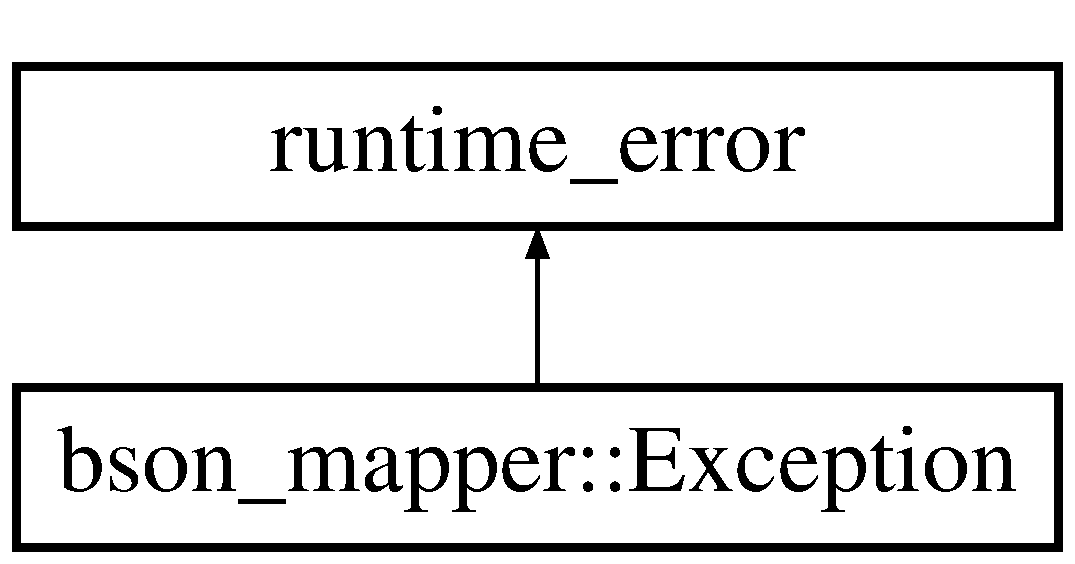
\includegraphics[height=2.000000cm]{structbson__mapper_1_1Exception}
\end{center}
\end{figure}


\subsection{Detailed Description}
An exception class thrown when things go wrong at runtime. 

The documentation for this struct was generated from the following file\+:\begin{DoxyCompactItemize}
\item 
src/bson\+\_\+mapper/bson\+\_\+archiver.\+hpp\end{DoxyCompactItemize}

\hypertarget{classmongo__odm_1_1ExpressionList}{}\section{mongo\+\_\+odm\+:\+:Expression\+List$<$ Head, Tail $>$ Class Template Reference}
\label{classmongo__odm_1_1ExpressionList}\index{mongo\+\_\+odm\+::\+Expression\+List$<$ Head, Tail $>$@{mongo\+\_\+odm\+::\+Expression\+List$<$ Head, Tail $>$}}
\subsection*{Public Member Functions}
\begin{DoxyCompactItemize}
\item 
constexpr \hyperlink{classmongo__odm_1_1ExpressionList_a77d2708484097a9aafa068cc7f1a9ebe}{Expression\+List} (const Head \&head, const Tail \&tail)
\begin{DoxyCompactList}\small\item\em Constructs an expression list. \end{DoxyCompactList}\item 
void \hyperlink{classmongo__odm_1_1ExpressionList_acce8b8732ff446bb9a36c64ec055f23f}{append\+\_\+to\+\_\+bson} (bsoncxx\+::builder\+::core \&builder) const 
\begin{DoxyCompactList}\small\item\em Appends this expression list to the given core builder by appending the first expression in the list, and then recursing on the rest of the list. \end{DoxyCompactList}\item 
\hyperlink{classmongo__odm_1_1ExpressionList_a09d23e240065afc839e4b791a7916163}{operator bsoncxx\+::document\+::view\+\_\+or\+\_\+value} () const 
\begin{DoxyCompactList}\small\item\em Casts the expression list to a B\+S\+ON query of the form \{ expr1, expr2, .... \end{DoxyCompactList}\end{DoxyCompactItemize}


\subsection{Constructor \& Destructor Documentation}
\index{mongo\+\_\+odm\+::\+Expression\+List@{mongo\+\_\+odm\+::\+Expression\+List}!Expression\+List@{Expression\+List}}
\index{Expression\+List@{Expression\+List}!mongo\+\_\+odm\+::\+Expression\+List@{mongo\+\_\+odm\+::\+Expression\+List}}
\subsubsection[{\texorpdfstring{Expression\+List(const Head \&head, const Tail \&tail)}{ExpressionList(const Head &head, const Tail &tail)}}]{\setlength{\rightskip}{0pt plus 5cm}template$<$typename Head , typename Tail $>$ constexpr {\bf mongo\+\_\+odm\+::\+Expression\+List}$<$ Head, Tail $>$\+::{\bf Expression\+List} (
\begin{DoxyParamCaption}
\item[{const Head \&}]{head, }
\item[{const Tail \&}]{tail}
\end{DoxyParamCaption}
)\hspace{0.3cm}{\ttfamily [inline]}}\hypertarget{classmongo__odm_1_1ExpressionList_a77d2708484097a9aafa068cc7f1a9ebe}{}\label{classmongo__odm_1_1ExpressionList_a77d2708484097a9aafa068cc7f1a9ebe}


Constructs an expression list. 


\begin{DoxyParams}{Parameters}
{\em head} & The first element in the list \\
\hline
{\em tail} & The remainder of the list \\
\hline
\end{DoxyParams}


\subsection{Member Function Documentation}
\index{mongo\+\_\+odm\+::\+Expression\+List@{mongo\+\_\+odm\+::\+Expression\+List}!append\+\_\+to\+\_\+bson@{append\+\_\+to\+\_\+bson}}
\index{append\+\_\+to\+\_\+bson@{append\+\_\+to\+\_\+bson}!mongo\+\_\+odm\+::\+Expression\+List@{mongo\+\_\+odm\+::\+Expression\+List}}
\subsubsection[{\texorpdfstring{append\+\_\+to\+\_\+bson(bsoncxx\+::builder\+::core \&builder) const }{append_to_bson(bsoncxx::builder::core &builder) const }}]{\setlength{\rightskip}{0pt plus 5cm}template$<$typename Head , typename Tail $>$ void {\bf mongo\+\_\+odm\+::\+Expression\+List}$<$ Head, Tail $>$\+::append\+\_\+to\+\_\+bson (
\begin{DoxyParamCaption}
\item[{bsoncxx\+::builder\+::core \&}]{builder}
\end{DoxyParamCaption}
) const\hspace{0.3cm}{\ttfamily [inline]}}\hypertarget{classmongo__odm_1_1ExpressionList_acce8b8732ff446bb9a36c64ec055f23f}{}\label{classmongo__odm_1_1ExpressionList_acce8b8732ff446bb9a36c64ec055f23f}


Appends this expression list to the given core builder by appending the first expression in the list, and then recursing on the rest of the list. 


\begin{DoxyParams}{Parameters}
{\em builder} & A basic B\+S\+ON core builder. \\
\hline
\end{DoxyParams}
\index{mongo\+\_\+odm\+::\+Expression\+List@{mongo\+\_\+odm\+::\+Expression\+List}!operator bsoncxx\+::document\+::view\+\_\+or\+\_\+value@{operator bsoncxx\+::document\+::view\+\_\+or\+\_\+value}}
\index{operator bsoncxx\+::document\+::view\+\_\+or\+\_\+value@{operator bsoncxx\+::document\+::view\+\_\+or\+\_\+value}!mongo\+\_\+odm\+::\+Expression\+List@{mongo\+\_\+odm\+::\+Expression\+List}}
\subsubsection[{\texorpdfstring{operator bsoncxx\+::document\+::view\+\_\+or\+\_\+value() const }{operator bsoncxx::document::view_or_value() const }}]{\setlength{\rightskip}{0pt plus 5cm}template$<$typename Head , typename Tail $>$ {\bf mongo\+\_\+odm\+::\+Expression\+List}$<$ Head, Tail $>$\+::operator bsoncxx\+::document\+::view\+\_\+or\+\_\+value (
\begin{DoxyParamCaption}
{}
\end{DoxyParamCaption}
) const\hspace{0.3cm}{\ttfamily [inline]}}\hypertarget{classmongo__odm_1_1ExpressionList_a09d23e240065afc839e4b791a7916163}{}\label{classmongo__odm_1_1ExpressionList_a09d23e240065afc839e4b791a7916163}


Casts the expression list to a B\+S\+ON query of the form \{ expr1, expr2, .... 

\} 

The documentation for this class was generated from the following file\+:\begin{DoxyCompactItemize}
\item 
src/mongo\+\_\+odm/query\+\_\+builder.\+hpp\end{DoxyCompactItemize}

\hypertarget{structmongo__odm_1_1FirstTypeIsTheSame}{}\section{mongo\+\_\+odm\+:\+:First\+Type\+Is\+The\+Same$<$ Ts $>$ Struct Template Reference}
\label{structmongo__odm_1_1FirstTypeIsTheSame}\index{mongo\+\_\+odm\+::\+First\+Type\+Is\+The\+Same$<$ Ts $>$@{mongo\+\_\+odm\+::\+First\+Type\+Is\+The\+Same$<$ Ts $>$}}


Helper type trait widget that helps properly forward arguments to \+\_\+id constructor.  




{\ttfamily \#include $<$model.\+hpp$>$}

Inheritance diagram for mongo\+\_\+odm\+:\+:First\+Type\+Is\+The\+Same$<$ Ts $>$\+:\begin{figure}[H]
\begin{center}
\leavevmode
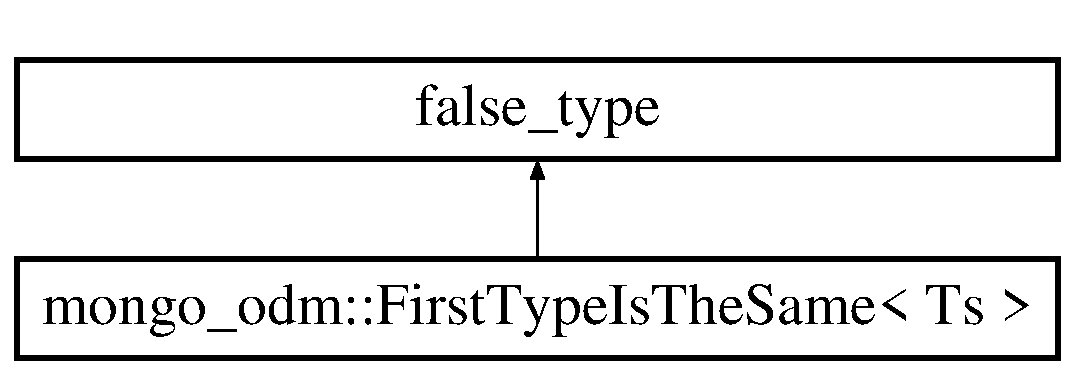
\includegraphics[height=2.000000cm]{structmongo__odm_1_1FirstTypeIsTheSame}
\end{center}
\end{figure}


\subsection{Detailed Description}
\subsubsection*{template$<$typename... Ts$>$\\*
struct mongo\+\_\+odm\+::\+First\+Type\+Is\+The\+Same$<$ Ts $>$}

Helper type trait widget that helps properly forward arguments to \+\_\+id constructor. 

First\+Type\+Is\+The\+Same$<$\+T1, T2, ...$>$\+::value will be true when T1 and T2 are of the same type, and false otherwise. 

The documentation for this struct was generated from the following file\+:\begin{DoxyCompactItemize}
\item 
src/mongo\+\_\+odm/model.\+hpp\end{DoxyCompactItemize}

\hypertarget{structmongo__odm_1_1FirstTypeIsTheSame_3_01T_00_01T2_00_01Ts_8_8_8_01_4}{}\section{mongo\+\_\+odm\+:\+:First\+Type\+Is\+The\+Same$<$ T, T2, Ts... $>$ Struct Template Reference}
\label{structmongo__odm_1_1FirstTypeIsTheSame_3_01T_00_01T2_00_01Ts_8_8_8_01_4}\index{mongo\+\_\+odm\+::\+First\+Type\+Is\+The\+Same$<$ T, T2, Ts... $>$@{mongo\+\_\+odm\+::\+First\+Type\+Is\+The\+Same$<$ T, T2, Ts... $>$}}
Inheritance diagram for mongo\+\_\+odm\+:\+:First\+Type\+Is\+The\+Same$<$ T, T2, Ts... $>$\+:\begin{figure}[H]
\begin{center}
\leavevmode
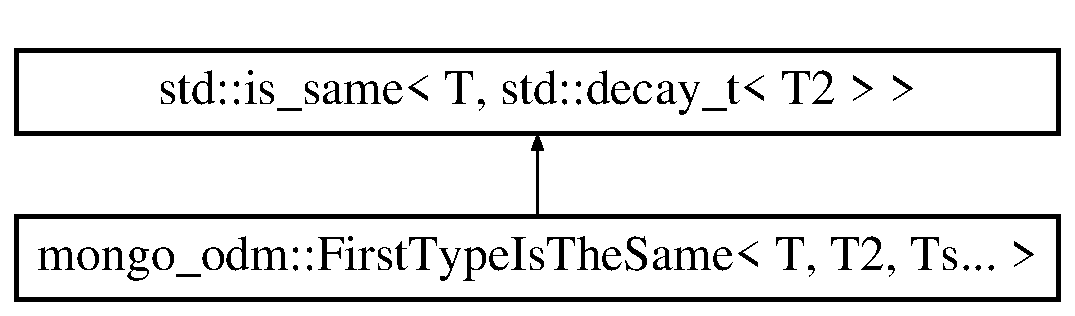
\includegraphics[height=2.000000cm]{structmongo__odm_1_1FirstTypeIsTheSame_3_01T_00_01T2_00_01Ts_8_8_8_01_4}
\end{center}
\end{figure}


The documentation for this struct was generated from the following file\+:\begin{DoxyCompactItemize}
\item 
src/mongo\+\_\+odm/model.\+hpp\end{DoxyCompactItemize}

\hypertarget{structmongo__odm_1_1hasField}{}\section{mongo\+\_\+odm\+:\+:has\+Field$<$ Base, T, N, M, bool $>$ Struct Template Reference}
\label{structmongo__odm_1_1hasField}\index{mongo\+\_\+odm\+::has\+Field$<$ Base, T, N, M, bool $>$@{mongo\+\_\+odm\+::has\+Field$<$ Base, T, N, M, bool $>$}}


\hyperlink{structmongo__odm_1_1hasField}{has\+Field} determines whether a type Base has a member of the given type T as the Nth member out of M total members which have name value pairs.  




{\ttfamily \#include $<$nvp.\+hpp$>$}

Inheritance diagram for mongo\+\_\+odm\+:\+:has\+Field$<$ Base, T, N, M, bool $>$\+:\begin{figure}[H]
\begin{center}
\leavevmode
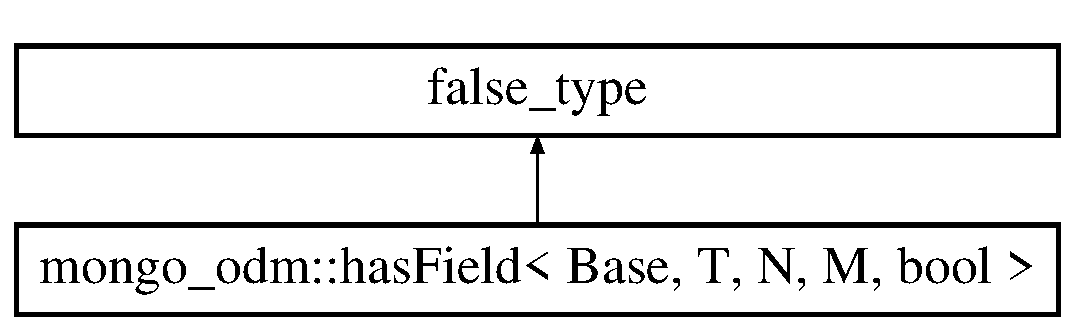
\includegraphics[height=2.000000cm]{structmongo__odm_1_1hasField}
\end{center}
\end{figure}


\subsection{Detailed Description}
\subsubsection*{template$<$typename Base, typename T, size\+\_\+t N, size\+\_\+t M, bool = (\+N $<$ M)$>$\\*
struct mongo\+\_\+odm\+::has\+Field$<$ Base, T, N, M, bool $>$}

\hyperlink{structmongo__odm_1_1hasField}{has\+Field} determines whether a type Base has a member of the given type T as the Nth member out of M total members which have name value pairs. 

The documentation for this struct was generated from the following file\+:\begin{DoxyCompactItemize}
\item 
src/mongo\+\_\+odm/nvp.\+hpp\end{DoxyCompactItemize}

\hypertarget{structmongo__odm_1_1hasField_3_01Base_00_01T_00_01N_00_01M_00_01true_01_4}{}\section{mongo\+\_\+odm\+:\+:has\+Field$<$ Base, T, N, M, true $>$ Struct Template Reference}
\label{structmongo__odm_1_1hasField_3_01Base_00_01T_00_01N_00_01M_00_01true_01_4}\index{mongo\+\_\+odm\+::has\+Field$<$ Base, T, N, M, true $>$@{mongo\+\_\+odm\+::has\+Field$<$ Base, T, N, M, true $>$}}
Inheritance diagram for mongo\+\_\+odm\+:\+:has\+Field$<$ Base, T, N, M, true $>$\+:\begin{figure}[H]
\begin{center}
\leavevmode
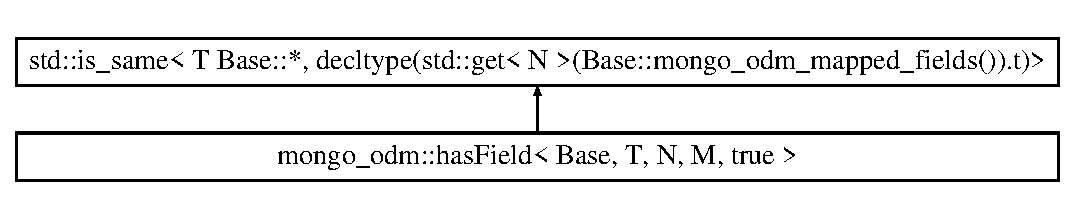
\includegraphics[height=2.000000cm]{structmongo__odm_1_1hasField_3_01Base_00_01T_00_01N_00_01M_00_01true_01_4}
\end{center}
\end{figure}


The documentation for this struct was generated from the following file\+:\begin{DoxyCompactItemize}
\item 
src/mongo\+\_\+odm/nvp.\+hpp\end{DoxyCompactItemize}

\hypertarget{structbson__mapper_1_1is__bson}{}\section{bson\+\_\+mapper\+:\+:is\+\_\+bson$<$ BsonT $>$ Struct Template Reference}
\label{structbson__mapper_1_1is__bson}\index{bson\+\_\+mapper\+::is\+\_\+bson$<$ Bson\+T $>$@{bson\+\_\+mapper\+::is\+\_\+bson$<$ Bson\+T $>$}}


A templated struct containing a bool value that specifies whether the provided template parameter is a B\+S\+ON type.  




{\ttfamily \#include $<$bson\+\_\+archiver.\+hpp$>$}



\subsection{Detailed Description}
\subsubsection*{template$<$class BsonT$>$\\*
struct bson\+\_\+mapper\+::is\+\_\+bson$<$ Bson\+T $>$}

A templated struct containing a bool value that specifies whether the provided template parameter is a B\+S\+ON type. 

The documentation for this struct was generated from the following file\+:\begin{DoxyCompactItemize}
\item 
src/bson\+\_\+mapper/bson\+\_\+archiver.\+hpp\end{DoxyCompactItemize}

\hypertarget{structbson__mapper_1_1is__bson__view}{}\section{bson\+\_\+mapper\+:\+:is\+\_\+bson\+\_\+view$<$ BsonT $>$ Struct Template Reference}
\label{structbson__mapper_1_1is__bson__view}\index{bson\+\_\+mapper\+::is\+\_\+bson\+\_\+view$<$ Bson\+T $>$@{bson\+\_\+mapper\+::is\+\_\+bson\+\_\+view$<$ Bson\+T $>$}}


A templated struct containing a bool value that specifies whether the provided template parameter is a B\+S\+ON type that contains a view.  




{\ttfamily \#include $<$bson\+\_\+archiver.\+hpp$>$}



\subsection{Detailed Description}
\subsubsection*{template$<$class BsonT$>$\\*
struct bson\+\_\+mapper\+::is\+\_\+bson\+\_\+view$<$ Bson\+T $>$}

A templated struct containing a bool value that specifies whether the provided template parameter is a B\+S\+ON type that contains a view. 

The documentation for this struct was generated from the following file\+:\begin{DoxyCompactItemize}
\item 
src/bson\+\_\+mapper/bson\+\_\+archiver.\+hpp\end{DoxyCompactItemize}

\hypertarget{structmongo__odm_1_1is__expression}{}\section{mongo\+\_\+odm\+:\+:is\+\_\+expression$<$ typename $>$ Struct Template Reference}
\label{structmongo__odm_1_1is__expression}\index{mongo\+\_\+odm\+::is\+\_\+expression$<$ typename $>$@{mongo\+\_\+odm\+::is\+\_\+expression$<$ typename $>$}}
Inheritance diagram for mongo\+\_\+odm\+:\+:is\+\_\+expression$<$ typename $>$\+:\begin{figure}[H]
\begin{center}
\leavevmode
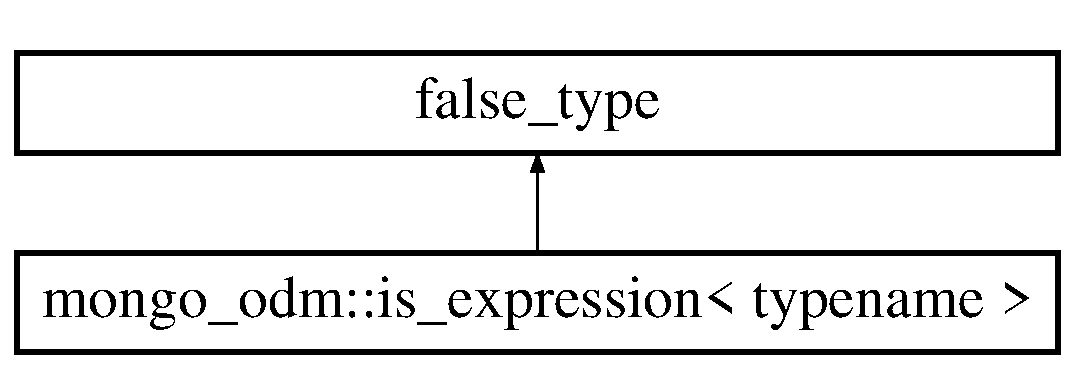
\includegraphics[height=2.000000cm]{structmongo__odm_1_1is__expression}
\end{center}
\end{figure}


The documentation for this struct was generated from the following file\+:\begin{DoxyCompactItemize}
\item 
src/mongo\+\_\+odm/query\+\_\+builder.\+hpp\end{DoxyCompactItemize}

\hypertarget{structmongo__odm_1_1is__expression_3_01BooleanExpr_3_01Expr1_00_01Expr2_01_4_01_4}{}\section{mongo\+\_\+odm\+:\+:is\+\_\+expression$<$ Boolean\+Expr$<$ Expr1, Expr2 $>$ $>$ Struct Template Reference}
\label{structmongo__odm_1_1is__expression_3_01BooleanExpr_3_01Expr1_00_01Expr2_01_4_01_4}\index{mongo\+\_\+odm\+::is\+\_\+expression$<$ Boolean\+Expr$<$ Expr1, Expr2 $>$ $>$@{mongo\+\_\+odm\+::is\+\_\+expression$<$ Boolean\+Expr$<$ Expr1, Expr2 $>$ $>$}}
Inheritance diagram for mongo\+\_\+odm\+:\+:is\+\_\+expression$<$ Boolean\+Expr$<$ Expr1, Expr2 $>$ $>$\+:\begin{figure}[H]
\begin{center}
\leavevmode
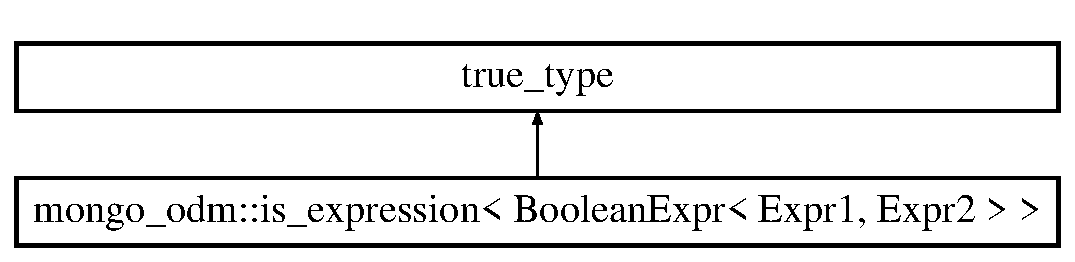
\includegraphics[height=2.000000cm]{structmongo__odm_1_1is__expression_3_01BooleanExpr_3_01Expr1_00_01Expr2_01_4_01_4}
\end{center}
\end{figure}


The documentation for this struct was generated from the following file\+:\begin{DoxyCompactItemize}
\item 
src/mongo\+\_\+odm/query\+\_\+builder.\+hpp\end{DoxyCompactItemize}

\hypertarget{structmongo__odm_1_1is__expression_3_01ComparisonExpr_3_01Base_00_01T_01_4_01_4}{}\section{mongo\+\_\+odm\+:\+:is\+\_\+expression$<$ Comparison\+Expr$<$ Base, T $>$ $>$ Struct Template Reference}
\label{structmongo__odm_1_1is__expression_3_01ComparisonExpr_3_01Base_00_01T_01_4_01_4}\index{mongo\+\_\+odm\+::is\+\_\+expression$<$ Comparison\+Expr$<$ Base, T $>$ $>$@{mongo\+\_\+odm\+::is\+\_\+expression$<$ Comparison\+Expr$<$ Base, T $>$ $>$}}
Inheritance diagram for mongo\+\_\+odm\+:\+:is\+\_\+expression$<$ Comparison\+Expr$<$ Base, T $>$ $>$\+:\begin{figure}[H]
\begin{center}
\leavevmode
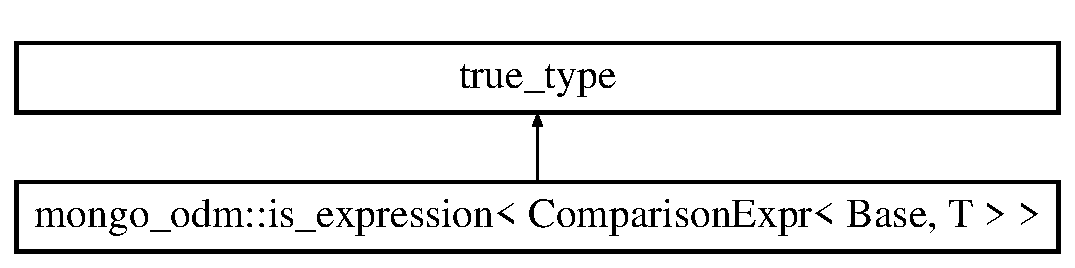
\includegraphics[height=2.000000cm]{structmongo__odm_1_1is__expression_3_01ComparisonExpr_3_01Base_00_01T_01_4_01_4}
\end{center}
\end{figure}


The documentation for this struct was generated from the following file\+:\begin{DoxyCompactItemize}
\item 
src/mongo\+\_\+odm/query\+\_\+builder.\+hpp\end{DoxyCompactItemize}

\hypertarget{structmongo__odm_1_1is__expression_3_01ExpressionList_3_01Head_00_01Tail_01_4_01_4}{}\section{mongo\+\_\+odm\+:\+:is\+\_\+expression$<$ Expression\+List$<$ Head, Tail $>$ $>$ Struct Template Reference}
\label{structmongo__odm_1_1is__expression_3_01ExpressionList_3_01Head_00_01Tail_01_4_01_4}\index{mongo\+\_\+odm\+::is\+\_\+expression$<$ Expression\+List$<$ Head, Tail $>$ $>$@{mongo\+\_\+odm\+::is\+\_\+expression$<$ Expression\+List$<$ Head, Tail $>$ $>$}}
Inheritance diagram for mongo\+\_\+odm\+:\+:is\+\_\+expression$<$ Expression\+List$<$ Head, Tail $>$ $>$\+:\begin{figure}[H]
\begin{center}
\leavevmode
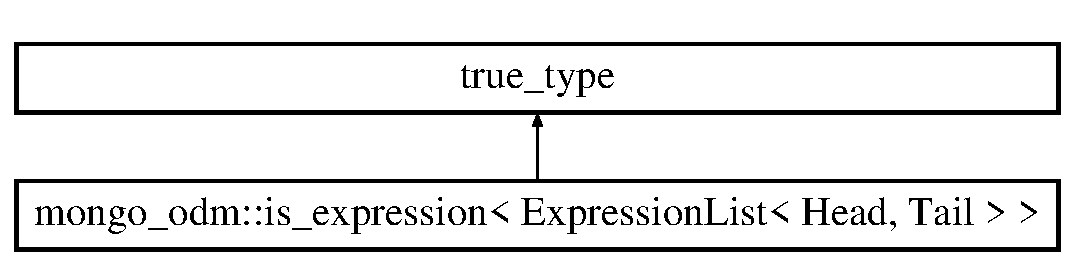
\includegraphics[height=2.000000cm]{structmongo__odm_1_1is__expression_3_01ExpressionList_3_01Head_00_01Tail_01_4_01_4}
\end{center}
\end{figure}


The documentation for this struct was generated from the following file\+:\begin{DoxyCompactItemize}
\item 
src/mongo\+\_\+odm/query\+\_\+builder.\+hpp\end{DoxyCompactItemize}

\hypertarget{structmongo__odm_1_1is__expression_3_01NotExpr_3_01Base_00_01T_01_4_01_4}{}\section{mongo\+\_\+odm\+:\+:is\+\_\+expression$<$ Not\+Expr$<$ Base, T $>$ $>$ Struct Template Reference}
\label{structmongo__odm_1_1is__expression_3_01NotExpr_3_01Base_00_01T_01_4_01_4}\index{mongo\+\_\+odm\+::is\+\_\+expression$<$ Not\+Expr$<$ Base, T $>$ $>$@{mongo\+\_\+odm\+::is\+\_\+expression$<$ Not\+Expr$<$ Base, T $>$ $>$}}
Inheritance diagram for mongo\+\_\+odm\+:\+:is\+\_\+expression$<$ Not\+Expr$<$ Base, T $>$ $>$\+:\begin{figure}[H]
\begin{center}
\leavevmode
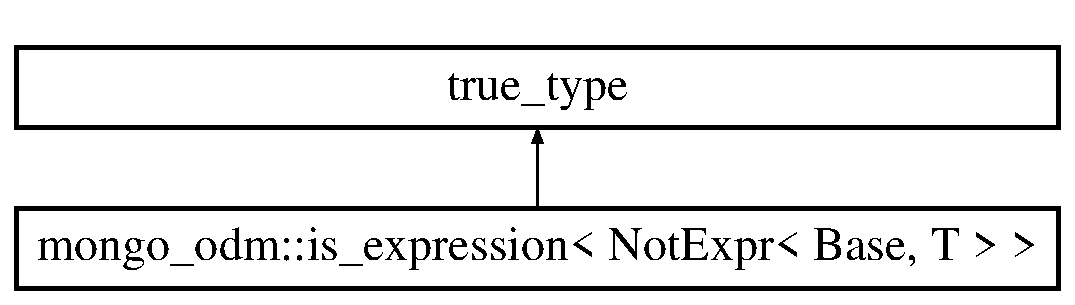
\includegraphics[height=2.000000cm]{structmongo__odm_1_1is__expression_3_01NotExpr_3_01Base_00_01T_01_4_01_4}
\end{center}
\end{figure}


The documentation for this struct was generated from the following file\+:\begin{DoxyCompactItemize}
\item 
src/mongo\+\_\+odm/query\+\_\+builder.\+hpp\end{DoxyCompactItemize}

\hypertarget{classmongo__odm_1_1deserializing__cursor_1_1iterator}{}\section{mongo\+\_\+odm\+:\+:deserializing\+\_\+cursor$<$ T $>$\+:\+:iterator Class Reference}
\label{classmongo__odm_1_1deserializing__cursor_1_1iterator}\index{mongo\+\_\+odm\+::deserializing\+\_\+cursor$<$ T $>$\+::iterator@{mongo\+\_\+odm\+::deserializing\+\_\+cursor$<$ T $>$\+::iterator}}
Inheritance diagram for mongo\+\_\+odm\+:\+:deserializing\+\_\+cursor$<$ T $>$\+:\+:iterator\+:\begin{figure}[H]
\begin{center}
\leavevmode
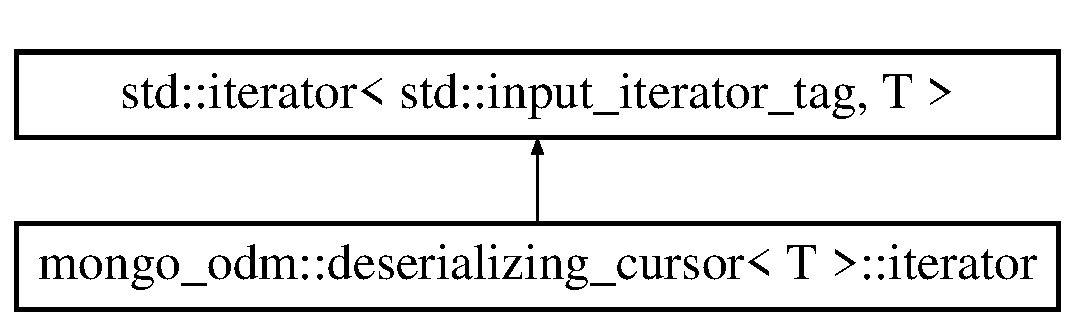
\includegraphics[height=2.000000cm]{classmongo__odm_1_1deserializing__cursor_1_1iterator}
\end{center}
\end{figure}
\subsection*{Public Member Functions}
\begin{DoxyCompactItemize}
\item 
T \hyperlink{classmongo__odm_1_1deserializing__cursor_1_1iterator_ad7b8718a44ef73460ed9196c719acaf6}{operator$\ast$} ()\hypertarget{classmongo__odm_1_1deserializing__cursor_1_1iterator_ad7b8718a44ef73460ed9196c719acaf6}{}\label{classmongo__odm_1_1deserializing__cursor_1_1iterator_ad7b8718a44ef73460ed9196c719acaf6}

\begin{DoxyCompactList}\small\item\em Returns a deserialized object that corresponds to the current document pointed to by the underlying collection cursor iterator. \end{DoxyCompactList}\end{DoxyCompactItemize}


The documentation for this class was generated from the following file\+:\begin{DoxyCompactItemize}
\item 
src/mongo\+\_\+odm/deserializing\+\_\+cursor.\+hpp\end{DoxyCompactItemize}

\hypertarget{classmongo__odm_1_1model}{}\section{mongo\+\_\+odm\+:\+:model$<$ T, Id\+Type $>$ Class Template Reference}
\label{classmongo__odm_1_1model}\index{mongo\+\_\+odm\+::model$<$ T, Id\+Type $>$@{mongo\+\_\+odm\+::model$<$ T, Id\+Type $>$}}
\subsection*{Public Member Functions}
\begin{DoxyCompactItemize}
\item 
{\footnotesize template$<$typename... Ts, typename  = std\+::enable\+\_\+if\+\_\+t$<$!\+First\+Type\+Is\+The\+Same$<$model, Ts...$>$\+::value$>$$>$ }\\\hyperlink{classmongo__odm_1_1model_ae00ec1da4db3b0851ccb3990a33a8f8e}{model} (Ts \&\&...ts)
\begin{DoxyCompactList}\small\item\em Forward the arguments to the constructor of Id\+Type. \end{DoxyCompactList}\item 
void \hyperlink{classmongo__odm_1_1model_a248cf30be3ee63741af5396a337b2694}{save} ()
\begin{DoxyCompactList}\small\item\em Performs an update in the database that saves the current T object instance to the collection mapped to this class. \end{DoxyCompactList}\item 
void \hyperlink{classmongo__odm_1_1model_a63b9538d2226531814bee3b7e7d26586}{remove} ()
\begin{DoxyCompactList}\small\item\em Deletes this object from the underlying collection. \end{DoxyCompactList}\end{DoxyCompactItemize}
\subsection*{Static Public Member Functions}
\begin{DoxyCompactItemize}
\item 
static const mongocxx\+::collection \hyperlink{classmongo__odm_1_1model_a889659470cbceaa2f9134ff383171e48}{collection} ()
\begin{DoxyCompactList}\small\item\em Returns a copy of the underlying collection. \end{DoxyCompactList}\item 
static void \hyperlink{classmongo__odm_1_1model_af47852c3aa1b8a9e5c07fa96c8530401}{drop} ()
\begin{DoxyCompactList}\small\item\em Drops the underlying collection and all its contained documents from the database. \end{DoxyCompactList}\item 
static void \hyperlink{classmongo__odm_1_1model_abff58cf53410faa6e0fe3ef820ca1612}{set\+Collection} (const mongocxx\+::collection \&coll)
\begin{DoxyCompactList}\small\item\em Sets the underlying mongocxx\+::collection used to store and load instances of T. \end{DoxyCompactList}\item 
static \hyperlink{classmongo__odm_1_1deserializing__cursor}{deserializing\+\_\+cursor}$<$ T $>$ \hyperlink{classmongo__odm_1_1model_a82419c85a1aa7de0de1c1202d4fafa2f}{find} (bsoncxx\+::document\+::view\+\_\+or\+\_\+value filter, const mongocxx\+::options\+::find \&options=mongocxx\+::options\+::find())
\begin{DoxyCompactList}\small\item\em Finds the documents in this collection which match the provided filter. \end{DoxyCompactList}\item 
static mongocxx\+::stdx\+::optional$<$ T $>$ \hyperlink{classmongo__odm_1_1model_a34b44af2a382b63b33e88dfb092e747c}{find\+\_\+one} (bsoncxx\+::document\+::view\+\_\+or\+\_\+value filter, const mongocxx\+::options\+::find \&options=mongocxx\+::options\+::find())
\begin{DoxyCompactList}\small\item\em Finds a single document in this collection that matches the provided filter. \end{DoxyCompactList}\end{DoxyCompactItemize}


\subsection{Constructor \& Destructor Documentation}
\index{mongo\+\_\+odm\+::model@{mongo\+\_\+odm\+::model}!model@{model}}
\index{model@{model}!mongo\+\_\+odm\+::model@{mongo\+\_\+odm\+::model}}
\subsubsection[{\texorpdfstring{model(\+Ts \&\&...\+ts)}{model(Ts &&...ts)}}]{\setlength{\rightskip}{0pt plus 5cm}template$<$typename T , typename Id\+Type  = bsoncxx\+::oid$>$ template$<$typename... Ts, typename  = std\+::enable\+\_\+if\+\_\+t$<$!\+First\+Type\+Is\+The\+Same$<$model, Ts...$>$\+::value$>$$>$ {\bf mongo\+\_\+odm\+::model}$<$ T, Id\+Type $>$\+::{\bf model} (
\begin{DoxyParamCaption}
\item[{Ts \&\&...}]{ts}
\end{DoxyParamCaption}
)\hspace{0.3cm}{\ttfamily [inline]}}\hypertarget{classmongo__odm_1_1model_ae00ec1da4db3b0851ccb3990a33a8f8e}{}\label{classmongo__odm_1_1model_ae00ec1da4db3b0851ccb3990a33a8f8e}


Forward the arguments to the constructor of Id\+Type. 

A std\+::enable\+\_\+if is included to disable the template for the copy constructor case so the default is used.


\begin{DoxyParams}{Parameters}
{\em ts} & The variadic pack of arguments to be forwarded to the constructor of Id\+Type. \\
\hline
\end{DoxyParams}


\subsection{Member Function Documentation}
\index{mongo\+\_\+odm\+::model@{mongo\+\_\+odm\+::model}!collection@{collection}}
\index{collection@{collection}!mongo\+\_\+odm\+::model@{mongo\+\_\+odm\+::model}}
\subsubsection[{\texorpdfstring{collection()}{collection()}}]{\setlength{\rightskip}{0pt plus 5cm}template$<$typename T , typename Id\+Type  = bsoncxx\+::oid$>$ static const mongocxx\+::collection {\bf mongo\+\_\+odm\+::model}$<$ T, Id\+Type $>$\+::collection (
\begin{DoxyParamCaption}
{}
\end{DoxyParamCaption}
)\hspace{0.3cm}{\ttfamily [inline]}, {\ttfamily [static]}}\hypertarget{classmongo__odm_1_1model_a889659470cbceaa2f9134ff383171e48}{}\label{classmongo__odm_1_1model_a889659470cbceaa2f9134ff383171e48}


Returns a copy of the underlying collection. 

\begin{DoxyReturn}{Returns}
A copy of the underlying mongocxx\+::collection that this class uses to store and load instances of T. 
\end{DoxyReturn}
\index{mongo\+\_\+odm\+::model@{mongo\+\_\+odm\+::model}!drop@{drop}}
\index{drop@{drop}!mongo\+\_\+odm\+::model@{mongo\+\_\+odm\+::model}}
\subsubsection[{\texorpdfstring{drop()}{drop()}}]{\setlength{\rightskip}{0pt plus 5cm}template$<$typename T , typename Id\+Type  = bsoncxx\+::oid$>$ static void {\bf mongo\+\_\+odm\+::model}$<$ T, Id\+Type $>$\+::drop (
\begin{DoxyParamCaption}
{}
\end{DoxyParamCaption}
)\hspace{0.3cm}{\ttfamily [inline]}, {\ttfamily [static]}}\hypertarget{classmongo__odm_1_1model_af47852c3aa1b8a9e5c07fa96c8530401}{}\label{classmongo__odm_1_1model_af47852c3aa1b8a9e5c07fa96c8530401}


Drops the underlying collection and all its contained documents from the database. 


\begin{DoxyExceptions}{Exceptions}
{\em exception\+::operation} & if the operation fails.\\
\hline
\end{DoxyExceptions}
\begin{DoxySeeAlso}{See also}
\href{https://docs.mongodb.com/manual/reference/method/db.collection.drop/}{\tt https\+://docs.\+mongodb.\+com/manual/reference/method/db.\+collection.\+drop/} 
\end{DoxySeeAlso}
\index{mongo\+\_\+odm\+::model@{mongo\+\_\+odm\+::model}!find@{find}}
\index{find@{find}!mongo\+\_\+odm\+::model@{mongo\+\_\+odm\+::model}}
\subsubsection[{\texorpdfstring{find(bsoncxx\+::document\+::view\+\_\+or\+\_\+value filter, const mongocxx\+::options\+::find \&options=mongocxx\+::options\+::find())}{find(bsoncxx::document::view_or_value filter, const mongocxx::options::find &options=mongocxx::options::find())}}]{\setlength{\rightskip}{0pt plus 5cm}template$<$typename T , typename Id\+Type  = bsoncxx\+::oid$>$ static {\bf deserializing\+\_\+cursor}$<$T$>$ {\bf mongo\+\_\+odm\+::model}$<$ T, Id\+Type $>$\+::find (
\begin{DoxyParamCaption}
\item[{bsoncxx\+::document\+::view\+\_\+or\+\_\+value}]{filter, }
\item[{const mongocxx\+::options\+::find \&}]{options = {\ttfamily mongocxx\+:\+:options\+:\+:find()}}
\end{DoxyParamCaption}
)\hspace{0.3cm}{\ttfamily [inline]}, {\ttfamily [static]}}\hypertarget{classmongo__odm_1_1model_a82419c85a1aa7de0de1c1202d4fafa2f}{}\label{classmongo__odm_1_1model_a82419c85a1aa7de0de1c1202d4fafa2f}


Finds the documents in this collection which match the provided filter. 


\begin{DoxyParams}{Parameters}
{\em filter} & Document view representing a document that should match the query. \\
\hline
{\em options} & Optional arguments, see mongocxx\+::options\+::find\\
\hline
\end{DoxyParams}
\begin{DoxyReturn}{Returns}
Cursor with deserialized objects from the collection. 
\end{DoxyReturn}

\begin{DoxyExceptions}{Exceptions}
{\em If} & the find failed, the returned cursor will throw mongocxx\+::exception\+::query when it is iterated.\\
\hline
\end{DoxyExceptions}
\begin{DoxySeeAlso}{See also}
\href{https://docs.mongodb.com/manual/tutorial/query-documents/}{\tt https\+://docs.\+mongodb.\+com/manual/tutorial/query-\/documents/} 
\end{DoxySeeAlso}
\index{mongo\+\_\+odm\+::model@{mongo\+\_\+odm\+::model}!find\+\_\+one@{find\+\_\+one}}
\index{find\+\_\+one@{find\+\_\+one}!mongo\+\_\+odm\+::model@{mongo\+\_\+odm\+::model}}
\subsubsection[{\texorpdfstring{find\+\_\+one(bsoncxx\+::document\+::view\+\_\+or\+\_\+value filter, const mongocxx\+::options\+::find \&options=mongocxx\+::options\+::find())}{find_one(bsoncxx::document::view_or_value filter, const mongocxx::options::find &options=mongocxx::options::find())}}]{\setlength{\rightskip}{0pt plus 5cm}template$<$typename T , typename Id\+Type  = bsoncxx\+::oid$>$ static mongocxx\+::stdx\+::optional$<$T$>$ {\bf mongo\+\_\+odm\+::model}$<$ T, Id\+Type $>$\+::find\+\_\+one (
\begin{DoxyParamCaption}
\item[{bsoncxx\+::document\+::view\+\_\+or\+\_\+value}]{filter, }
\item[{const mongocxx\+::options\+::find \&}]{options = {\ttfamily mongocxx\+:\+:options\+:\+:find()}}
\end{DoxyParamCaption}
)\hspace{0.3cm}{\ttfamily [inline]}, {\ttfamily [static]}}\hypertarget{classmongo__odm_1_1model_a34b44af2a382b63b33e88dfb092e747c}{}\label{classmongo__odm_1_1model_a34b44af2a382b63b33e88dfb092e747c}


Finds a single document in this collection that matches the provided filter. 


\begin{DoxyParams}{Parameters}
{\em filter} & Document view representing a document that should match the query. \\
\hline
{\em options} & Optional arguments, see mongocxx\+::options\+::find\\
\hline
\end{DoxyParams}
\begin{DoxyReturn}{Returns}
An optional object that matched the filter. 
\end{DoxyReturn}

\begin{DoxyExceptions}{Exceptions}
{\em mongocxx\+::exception\+::query} & if the operation fails.\\
\hline
\end{DoxyExceptions}
\begin{DoxySeeAlso}{See also}
\href{https://docs.mongodb.com/manual/tutorial/query-documents/}{\tt https\+://docs.\+mongodb.\+com/manual/tutorial/query-\/documents/} 
\end{DoxySeeAlso}
\index{mongo\+\_\+odm\+::model@{mongo\+\_\+odm\+::model}!remove@{remove}}
\index{remove@{remove}!mongo\+\_\+odm\+::model@{mongo\+\_\+odm\+::model}}
\subsubsection[{\texorpdfstring{remove()}{remove()}}]{\setlength{\rightskip}{0pt plus 5cm}template$<$typename T , typename Id\+Type  = bsoncxx\+::oid$>$ void {\bf mongo\+\_\+odm\+::model}$<$ T, Id\+Type $>$\+::remove (
\begin{DoxyParamCaption}
{}
\end{DoxyParamCaption}
)\hspace{0.3cm}{\ttfamily [inline]}}\hypertarget{classmongo__odm_1_1model_a63b9538d2226531814bee3b7e7d26586}{}\label{classmongo__odm_1_1model_a63b9538d2226531814bee3b7e7d26586}


Deletes this object from the underlying collection. 

In the terms of the C\+R\+UD specification, this uses delete\+One with the \+\_\+id as the sole argument to the query filter.

\begin{DoxySeeAlso}{See also}
\href{https://docs.mongodb.com/manual/reference/method/db.collection.deleteOne/}{\tt https\+://docs.\+mongodb.\+com/manual/reference/method/db.\+collection.\+delete\+One/} 
\end{DoxySeeAlso}
\index{mongo\+\_\+odm\+::model@{mongo\+\_\+odm\+::model}!save@{save}}
\index{save@{save}!mongo\+\_\+odm\+::model@{mongo\+\_\+odm\+::model}}
\subsubsection[{\texorpdfstring{save()}{save()}}]{\setlength{\rightskip}{0pt plus 5cm}template$<$typename T , typename Id\+Type  = bsoncxx\+::oid$>$ void {\bf mongo\+\_\+odm\+::model}$<$ T, Id\+Type $>$\+::save (
\begin{DoxyParamCaption}
{}
\end{DoxyParamCaption}
)\hspace{0.3cm}{\ttfamily [inline]}}\hypertarget{classmongo__odm_1_1model_a248cf30be3ee63741af5396a337b2694}{}\label{classmongo__odm_1_1model_a248cf30be3ee63741af5396a337b2694}


Performs an update in the database that saves the current T object instance to the collection mapped to this class. 

In the terms of the C\+R\+UD specification, this uses update\+One with the \+\_\+id as the sole argument to the query filter, the T object serialized to dotted notation B\+S\+ON as the \$set operand, and upsert=true so that objects that aren\textquotesingle{}t already in the collection are automatically inserted.

\begin{DoxySeeAlso}{See also}
\href{https://docs.mongodb.com/manual/reference/method/db.collection.updateOne/}{\tt https\+://docs.\+mongodb.\+com/manual/reference/method/db.\+collection.\+update\+One/} 
\end{DoxySeeAlso}
\index{mongo\+\_\+odm\+::model@{mongo\+\_\+odm\+::model}!set\+Collection@{set\+Collection}}
\index{set\+Collection@{set\+Collection}!mongo\+\_\+odm\+::model@{mongo\+\_\+odm\+::model}}
\subsubsection[{\texorpdfstring{set\+Collection(const mongocxx\+::collection \&coll)}{setCollection(const mongocxx::collection &coll)}}]{\setlength{\rightskip}{0pt plus 5cm}template$<$typename T , typename Id\+Type  = bsoncxx\+::oid$>$ static void {\bf mongo\+\_\+odm\+::model}$<$ T, Id\+Type $>$\+::set\+Collection (
\begin{DoxyParamCaption}
\item[{const mongocxx\+::collection \&}]{coll}
\end{DoxyParamCaption}
)\hspace{0.3cm}{\ttfamily [inline]}, {\ttfamily [static]}}\hypertarget{classmongo__odm_1_1model_abff58cf53410faa6e0fe3ef820ca1612}{}\label{classmongo__odm_1_1model_abff58cf53410faa6e0fe3ef820ca1612}


Sets the underlying mongocxx\+::collection used to store and load instances of T. 


\begin{DoxyParams}{Parameters}
{\em coll} & The mongocxx\+::collection object to be mapped to this class.\\
\hline
\end{DoxyParams}
\begin{DoxyWarning}{Warning}
This must be called with a new mongocxx\+::collection instance for every thread for the O\+DM to be thread-\/safe.

The parent mongocxx\+::client from which the mongocxx\+::collection argument was created must outlive any of this model\textquotesingle{}s C\+R\+UD methods. If the client object goes out of scope, a new collection must be passed to this method before using any C\+R\+UD methods. 
\end{DoxyWarning}


The documentation for this class was generated from the following file\+:\begin{DoxyCompactItemize}
\item 
src/mongo\+\_\+odm/model.\+hpp\end{DoxyCompactItemize}

\hypertarget{classmongo__odm_1_1NotExpr}{}\section{mongo\+\_\+odm\+:\+:Not\+Expr$<$ Base, T $>$ Class Template Reference}
\label{classmongo__odm_1_1NotExpr}\index{mongo\+\_\+odm\+::\+Not\+Expr$<$ Base, T $>$@{mongo\+\_\+odm\+::\+Not\+Expr$<$ Base, T $>$}}


This represents an expression with the \$not operator, which wraps a comparison expression and negates it.  




{\ttfamily \#include $<$query\+\_\+builder.\+hpp$>$}

\subsection*{Public Member Functions}
\begin{DoxyCompactItemize}
\item 
constexpr \hyperlink{classmongo__odm_1_1NotExpr_a817dba48751e400a44e83c79ac57872f}{Not\+Expr} (const \hyperlink{classmongo__odm_1_1ComparisonExpr}{Comparison\+Expr}$<$ Base, T $>$ \&expr)
\begin{DoxyCompactList}\small\item\em Creates a \$not expression taht negates the given comparison expression. \end{DoxyCompactList}\item 
void \hyperlink{classmongo__odm_1_1NotExpr_aee3b9cef41a1fa5f4e60e141cefd1357}{append\+\_\+to\+\_\+bson} (bsoncxx\+::builder\+::core \&builder) const 
\begin{DoxyCompactList}\small\item\em Appends this expression to a B\+S\+ON core builder, as a key-\/value pair of the form \char`\"{}key\+: \{\$not\+: \{\$cmp\+: val\}\}\char`\"{}. \end{DoxyCompactList}\item 
\hyperlink{classmongo__odm_1_1NotExpr_a6f2e9d9b79c21dafbf30f05d231ee52c}{operator bsoncxx\+::document\+::view\+\_\+or\+\_\+value} () const 
\begin{DoxyCompactList}\small\item\em Converts the expression to a B\+S\+ON filter for a query. \end{DoxyCompactList}\end{DoxyCompactItemize}


\subsection{Detailed Description}
\subsubsection*{template$<$typename Base, typename T$>$\\*
class mongo\+\_\+odm\+::\+Not\+Expr$<$ Base, T $>$}

This represents an expression with the \$not operator, which wraps a comparison expression and negates it. 

\subsection{Constructor \& Destructor Documentation}
\index{mongo\+\_\+odm\+::\+Not\+Expr@{mongo\+\_\+odm\+::\+Not\+Expr}!Not\+Expr@{Not\+Expr}}
\index{Not\+Expr@{Not\+Expr}!mongo\+\_\+odm\+::\+Not\+Expr@{mongo\+\_\+odm\+::\+Not\+Expr}}
\subsubsection[{\texorpdfstring{Not\+Expr(const Comparison\+Expr$<$ Base, T $>$ \&expr)}{NotExpr(const ComparisonExpr< Base, T > &expr)}}]{\setlength{\rightskip}{0pt plus 5cm}template$<$typename Base , typename T $>$ constexpr {\bf mongo\+\_\+odm\+::\+Not\+Expr}$<$ Base, T $>$\+::{\bf Not\+Expr} (
\begin{DoxyParamCaption}
\item[{const {\bf Comparison\+Expr}$<$ Base, T $>$ \&}]{expr}
\end{DoxyParamCaption}
)\hspace{0.3cm}{\ttfamily [inline]}}\hypertarget{classmongo__odm_1_1NotExpr_a817dba48751e400a44e83c79ac57872f}{}\label{classmongo__odm_1_1NotExpr_a817dba48751e400a44e83c79ac57872f}


Creates a \$not expression taht negates the given comparison expression. 


\begin{DoxyParams}{Parameters}
{\em expr} & A comparison expression \\
\hline
\end{DoxyParams}


\subsection{Member Function Documentation}
\index{mongo\+\_\+odm\+::\+Not\+Expr@{mongo\+\_\+odm\+::\+Not\+Expr}!append\+\_\+to\+\_\+bson@{append\+\_\+to\+\_\+bson}}
\index{append\+\_\+to\+\_\+bson@{append\+\_\+to\+\_\+bson}!mongo\+\_\+odm\+::\+Not\+Expr@{mongo\+\_\+odm\+::\+Not\+Expr}}
\subsubsection[{\texorpdfstring{append\+\_\+to\+\_\+bson(bsoncxx\+::builder\+::core \&builder) const }{append_to_bson(bsoncxx::builder::core &builder) const }}]{\setlength{\rightskip}{0pt plus 5cm}template$<$typename Base , typename T $>$ void {\bf mongo\+\_\+odm\+::\+Not\+Expr}$<$ Base, T $>$\+::append\+\_\+to\+\_\+bson (
\begin{DoxyParamCaption}
\item[{bsoncxx\+::builder\+::core \&}]{builder}
\end{DoxyParamCaption}
) const\hspace{0.3cm}{\ttfamily [inline]}}\hypertarget{classmongo__odm_1_1NotExpr_aee3b9cef41a1fa5f4e60e141cefd1357}{}\label{classmongo__odm_1_1NotExpr_aee3b9cef41a1fa5f4e60e141cefd1357}


Appends this expression to a B\+S\+ON core builder, as a key-\/value pair of the form \char`\"{}key\+: \{\$not\+: \{\$cmp\+: val\}\}\char`\"{}. 


\begin{DoxyParams}{Parameters}
{\em builder} & a B\+S\+ON core builder \\
\hline
\end{DoxyParams}
\index{mongo\+\_\+odm\+::\+Not\+Expr@{mongo\+\_\+odm\+::\+Not\+Expr}!operator bsoncxx\+::document\+::view\+\_\+or\+\_\+value@{operator bsoncxx\+::document\+::view\+\_\+or\+\_\+value}}
\index{operator bsoncxx\+::document\+::view\+\_\+or\+\_\+value@{operator bsoncxx\+::document\+::view\+\_\+or\+\_\+value}!mongo\+\_\+odm\+::\+Not\+Expr@{mongo\+\_\+odm\+::\+Not\+Expr}}
\subsubsection[{\texorpdfstring{operator bsoncxx\+::document\+::view\+\_\+or\+\_\+value() const }{operator bsoncxx::document::view_or_value() const }}]{\setlength{\rightskip}{0pt plus 5cm}template$<$typename Base , typename T $>$ {\bf mongo\+\_\+odm\+::\+Not\+Expr}$<$ Base, T $>$\+::operator bsoncxx\+::document\+::view\+\_\+or\+\_\+value (
\begin{DoxyParamCaption}
{}
\end{DoxyParamCaption}
) const\hspace{0.3cm}{\ttfamily [inline]}}\hypertarget{classmongo__odm_1_1NotExpr_a6f2e9d9b79c21dafbf30f05d231ee52c}{}\label{classmongo__odm_1_1NotExpr_a6f2e9d9b79c21dafbf30f05d231ee52c}


Converts the expression to a B\+S\+ON filter for a query. 

The format of the B\+S\+ON is \char`\"{}\{key\+: \{\$not\+: \{\$cmp\+: val\}\}\}\char`\"{}. 

The documentation for this class was generated from the following file\+:\begin{DoxyCompactItemize}
\item 
src/mongo\+\_\+odm/query\+\_\+builder.\+hpp\end{DoxyCompactItemize}

\hypertarget{structmongo__odm_1_1Nvp}{}\section{mongo\+\_\+odm\+:\+:Nvp$<$ Base, T $>$ Struct Template Reference}
\label{structmongo__odm_1_1Nvp}\index{mongo\+\_\+odm\+::\+Nvp$<$ Base, T $>$@{mongo\+\_\+odm\+::\+Nvp$<$ Base, T $>$}}


An object that represents a name-\/value pair of a member in an object.  




{\ttfamily \#include $<$nvp.\+hpp$>$}

\subsection*{Public Member Functions}
\begin{DoxyCompactItemize}
\item 
constexpr \hyperlink{structmongo__odm_1_1Nvp_a0892863bcb5093550a0f3bfad3a16580}{Nvp} (T Base\+::$\ast$t, const char $\ast$name)
\begin{DoxyCompactList}\small\item\em Create a name-\/value pair from a member pointer and a name. \end{DoxyCompactList}\end{DoxyCompactItemize}


\subsection{Detailed Description}
\subsubsection*{template$<$typename Base, typename T$>$\\*
struct mongo\+\_\+odm\+::\+Nvp$<$ Base, T $>$}

An object that represents a name-\/value pair of a member in an object. 

It is templated on the class of the member and its type. 

\subsection{Constructor \& Destructor Documentation}
\index{mongo\+\_\+odm\+::\+Nvp@{mongo\+\_\+odm\+::\+Nvp}!Nvp@{Nvp}}
\index{Nvp@{Nvp}!mongo\+\_\+odm\+::\+Nvp@{mongo\+\_\+odm\+::\+Nvp}}
\subsubsection[{\texorpdfstring{Nvp(\+T Base\+::$\ast$t, const char $\ast$name)}{Nvp(T Base::*t, const char *name)}}]{\setlength{\rightskip}{0pt plus 5cm}template$<$typename Base, typename T$>$ constexpr {\bf mongo\+\_\+odm\+::\+Nvp}$<$ Base, T $>$\+::{\bf Nvp} (
\begin{DoxyParamCaption}
\item[{T Base\+::$\ast$}]{t, }
\item[{const char $\ast$}]{name}
\end{DoxyParamCaption}
)\hspace{0.3cm}{\ttfamily [inline]}}\hypertarget{structmongo__odm_1_1Nvp_a0892863bcb5093550a0f3bfad3a16580}{}\label{structmongo__odm_1_1Nvp_a0892863bcb5093550a0f3bfad3a16580}


Create a name-\/value pair from a member pointer and a name. 


\begin{DoxyParams}{Parameters}
{\em t} & A pointer to the member \\
\hline
{\em name} & The name of the member \\
\hline
\end{DoxyParams}


The documentation for this struct was generated from the following file\+:\begin{DoxyCompactItemize}
\item 
src/mongo\+\_\+odm/nvp.\+hpp\end{DoxyCompactItemize}

\hypertarget{classmongo__odm_1_1odm__collection}{}\section{mongo\+\_\+odm\+:\+:odm\+\_\+collection$<$ T $>$ Class Template Reference}
\label{classmongo__odm_1_1odm__collection}\index{mongo\+\_\+odm\+::odm\+\_\+collection$<$ T $>$@{mongo\+\_\+odm\+::odm\+\_\+collection$<$ T $>$}}
\subsection*{Public Member Functions}
\begin{DoxyCompactItemize}
\item 
mongocxx\+::collection \hyperlink{classmongo__odm_1_1odm__collection_a65bf78cfb9fe5e977d5a9fe49bfcf387}{collection} ()
\begin{DoxyCompactList}\small\item\em Returns a copy of the underlying collection. \end{DoxyCompactList}\item 
{\footnotesize template$<$class Result  = T$>$ }\\\hyperlink{classmongo__odm_1_1deserializing__cursor}{deserializing\+\_\+cursor}$<$ Result $>$ \hyperlink{classmongo__odm_1_1odm__collection_a1be075e3d2b05b4bd328050d3566806c}{aggregate} (const mongocxx\+::pipeline \&pipeline, const mongocxx\+::options\+::aggregate \&options=mongocxx\+::options\+::aggregate())
\begin{DoxyCompactList}\small\item\em Runs an aggregation framework pipeline against this collection, and returns the results as de-\/serialized objects. \end{DoxyCompactList}\item 
\hyperlink{classmongo__odm_1_1deserializing__cursor}{deserializing\+\_\+cursor}$<$ T $>$ \hyperlink{classmongo__odm_1_1odm__collection_aef03132e2d00396555832734c75f43a1}{find} (bsoncxx\+::document\+::view\+\_\+or\+\_\+value filter, const mongocxx\+::options\+::find \&options=mongocxx\+::options\+::find())
\begin{DoxyCompactList}\small\item\em Finds the documents in this collection which match the provided filter. \end{DoxyCompactList}\item 
mongocxx\+::stdx\+::optional$<$ T $>$ \hyperlink{classmongo__odm_1_1odm__collection_a76f81952f53bacb0e4516abe3d680230}{find\+\_\+one} (bsoncxx\+::document\+::view\+\_\+or\+\_\+value filter, const mongocxx\+::options\+::find \&options=mongocxx\+::options\+::find())
\begin{DoxyCompactList}\small\item\em Finds a single document in this collection that match the provided filter. \end{DoxyCompactList}\item 
mongocxx\+::stdx\+::optional$<$ T $>$ \hyperlink{classmongo__odm_1_1odm__collection_a7b07969d21159f5dad3f86c5b37c6581}{find\+\_\+one\+\_\+and\+\_\+delete} (bsoncxx\+::document\+::view\+\_\+or\+\_\+value filter, const mongocxx\+::options\+::find\+\_\+one\+\_\+and\+\_\+delete \&options=mongocxx\+::options\+::find\+\_\+one\+\_\+and\+\_\+delete())
\begin{DoxyCompactList}\small\item\em Finds a single document matching the filter, deletes it, and returns the original as a deserialized object. \end{DoxyCompactList}\item 
mongocxx\+::stdx\+::optional$<$ T $>$ \hyperlink{classmongo__odm_1_1odm__collection_adbcbf110fd4b3d14f70206020eee24d3}{find\+\_\+one\+\_\+and\+\_\+replace} (bsoncxx\+::document\+::view\+\_\+or\+\_\+value filter, const T \&replacement, const mongocxx\+::options\+::find\+\_\+one\+\_\+and\+\_\+replace \&options=mongocxx\+::options\+::find\+\_\+one\+\_\+and\+\_\+replace())
\begin{DoxyCompactList}\small\item\em Finds a single document matching the filter, replaces it, and returns either the original or the replacement document as a deserialized object. \end{DoxyCompactList}\item 
mongocxx\+::stdx\+::optional$<$ mongocxx\+::result\+::insert\+\_\+one $>$ \hyperlink{classmongo__odm_1_1odm__collection_af11f78449ec0938caa49346da8eed19d}{insert\+\_\+one} (T obj, const mongocxx\+::options\+::insert \&options=mongocxx\+::options\+::insert())
\begin{DoxyCompactList}\small\item\em Inserts a single serializable object into the collection. \end{DoxyCompactList}\item 
{\footnotesize template$<$typename container\+\_\+type $>$ }\\mongocxx\+::stdx\+::optional$<$ mongocxx\+::result\+::insert\+\_\+many $>$ \hyperlink{classmongo__odm_1_1odm__collection_a9503db6dacc66f8af5466bd22479a90e}{insert\+\_\+many} (const container\+\_\+type \&container, const mongocxx\+::options\+::insert \&options=mongocxx\+::options\+::insert())
\begin{DoxyCompactList}\small\item\em Inserts multiple serializable objects into the collection. \end{DoxyCompactList}\item 
{\footnotesize template$<$typename object\+\_\+iterator\+\_\+type $>$ }\\mongocxx\+::stdx\+::optional$<$ mongocxx\+::result\+::insert\+\_\+many $>$ \hyperlink{classmongo__odm_1_1odm__collection_a411c5e06bd3dab97a15ee478f6dae540}{insert\+\_\+many} (object\+\_\+iterator\+\_\+type begin, object\+\_\+iterator\+\_\+type end, const mongocxx\+::options\+::insert \&options=mongocxx\+::options\+::insert())
\begin{DoxyCompactList}\small\item\em Inserts multiple serializable objects into the collection. \end{DoxyCompactList}\item 
mongocxx\+::stdx\+::optional$<$ mongocxx\+::result\+::replace\+\_\+one $>$ \hyperlink{classmongo__odm_1_1odm__collection_adf1ed50140b16bde3bef54a6f701e1a6}{replace\+\_\+one} (bsoncxx\+::document\+::view\+\_\+or\+\_\+value filter, const T \&replacement, const mongocxx\+::options\+::update \&options=mongocxx\+::options\+::update())
\begin{DoxyCompactList}\small\item\em Replaces a single document matching the provided filter in this collection. \end{DoxyCompactList}\end{DoxyCompactItemize}


\subsection{Member Function Documentation}
\index{mongo\+\_\+odm\+::odm\+\_\+collection@{mongo\+\_\+odm\+::odm\+\_\+collection}!aggregate@{aggregate}}
\index{aggregate@{aggregate}!mongo\+\_\+odm\+::odm\+\_\+collection@{mongo\+\_\+odm\+::odm\+\_\+collection}}
\subsubsection[{\texorpdfstring{aggregate(const mongocxx\+::pipeline \&pipeline, const mongocxx\+::options\+::aggregate \&options=mongocxx\+::options\+::aggregate())}{aggregate(const mongocxx::pipeline &pipeline, const mongocxx::options::aggregate &options=mongocxx::options::aggregate())}}]{\setlength{\rightskip}{0pt plus 5cm}template$<$class T$>$ template$<$class Result  = T$>$ {\bf deserializing\+\_\+cursor}$<$Result$>$ {\bf mongo\+\_\+odm\+::odm\+\_\+collection}$<$ T $>$\+::aggregate (
\begin{DoxyParamCaption}
\item[{const mongocxx\+::pipeline \&}]{pipeline, }
\item[{const mongocxx\+::options\+::aggregate \&}]{options = {\ttfamily mongocxx\+:\+:options\+:\+:aggregate()}}
\end{DoxyParamCaption}
)\hspace{0.3cm}{\ttfamily [inline]}}\hypertarget{classmongo__odm_1_1odm__collection_a1be075e3d2b05b4bd328050d3566806c}{}\label{classmongo__odm_1_1odm__collection_a1be075e3d2b05b4bd328050d3566806c}


Runs an aggregation framework pipeline against this collection, and returns the results as de-\/serialized objects. 

This function is templated on the result\textquotesingle{}s type, which is not necessarily the same as the type of the documents in the colleciton.


\begin{DoxyTemplParams}{Template Parameters}
{\em Result} & -\/ The type of the aggregation result. \\
\hline
\end{DoxyTemplParams}

\begin{DoxyParams}{Parameters}
{\em pipeline} & The pipeline of aggregation operations to perform. \\
\hline
{\em options} & Optional arguments, see mongocxx\+::mongocxx\+::options\+::aggregate.\\
\hline
\end{DoxyParams}
\begin{DoxyReturn}{Returns}
A deserializing\+\_\+cursor$<$\+Result$>$ with the results. 
\end{DoxyReturn}

\begin{DoxyExceptions}{Exceptions}
{\em If} & the operation failed, the returned cursor will throw an mongocxx\+::exception\+::query when it is iterated.\\
\hline
\end{DoxyExceptions}
\begin{DoxySeeAlso}{See also}
\href{http://docs.mongodb.org/manual/reference/command/aggregate/}{\tt http\+://docs.\+mongodb.\+org/manual/reference/command/aggregate/} 
\end{DoxySeeAlso}
\index{mongo\+\_\+odm\+::odm\+\_\+collection@{mongo\+\_\+odm\+::odm\+\_\+collection}!collection@{collection}}
\index{collection@{collection}!mongo\+\_\+odm\+::odm\+\_\+collection@{mongo\+\_\+odm\+::odm\+\_\+collection}}
\subsubsection[{\texorpdfstring{collection()}{collection()}}]{\setlength{\rightskip}{0pt plus 5cm}template$<$class T$>$ mongocxx\+::collection {\bf mongo\+\_\+odm\+::odm\+\_\+collection}$<$ T $>$\+::collection (
\begin{DoxyParamCaption}
{}
\end{DoxyParamCaption}
)\hspace{0.3cm}{\ttfamily [inline]}}\hypertarget{classmongo__odm_1_1odm__collection_a65bf78cfb9fe5e977d5a9fe49bfcf387}{}\label{classmongo__odm_1_1odm__collection_a65bf78cfb9fe5e977d5a9fe49bfcf387}


Returns a copy of the underlying collection. 

\begin{DoxyReturn}{Returns}
The mongocxx\+::collection that this object wraps 
\end{DoxyReturn}
\index{mongo\+\_\+odm\+::odm\+\_\+collection@{mongo\+\_\+odm\+::odm\+\_\+collection}!find@{find}}
\index{find@{find}!mongo\+\_\+odm\+::odm\+\_\+collection@{mongo\+\_\+odm\+::odm\+\_\+collection}}
\subsubsection[{\texorpdfstring{find(bsoncxx\+::document\+::view\+\_\+or\+\_\+value filter, const mongocxx\+::options\+::find \&options=mongocxx\+::options\+::find())}{find(bsoncxx::document::view_or_value filter, const mongocxx::options::find &options=mongocxx::options::find())}}]{\setlength{\rightskip}{0pt plus 5cm}template$<$class T$>$ {\bf deserializing\+\_\+cursor}$<$T$>$ {\bf mongo\+\_\+odm\+::odm\+\_\+collection}$<$ T $>$\+::find (
\begin{DoxyParamCaption}
\item[{bsoncxx\+::document\+::view\+\_\+or\+\_\+value}]{filter, }
\item[{const mongocxx\+::options\+::find \&}]{options = {\ttfamily mongocxx\+:\+:options\+:\+:find()}}
\end{DoxyParamCaption}
)\hspace{0.3cm}{\ttfamily [inline]}}\hypertarget{classmongo__odm_1_1odm__collection_aef03132e2d00396555832734c75f43a1}{}\label{classmongo__odm_1_1odm__collection_aef03132e2d00396555832734c75f43a1}


Finds the documents in this collection which match the provided filter. 


\begin{DoxyParams}{Parameters}
{\em filter} & Document view representing a document that should match the query. \\
\hline
{\em options} & Optional arguments, see mongocxx\+::options\+::find\\
\hline
\end{DoxyParams}
\begin{DoxyReturn}{Returns}
Cursor with deserialized objects from the collection. 
\end{DoxyReturn}

\begin{DoxyExceptions}{Exceptions}
{\em If} & the find failed, the returned cursor will throw mongocxx\+::exception\+::query when it is iterated.\\
\hline
\end{DoxyExceptions}
\begin{DoxySeeAlso}{See also}
\href{http://docs.mongodb.org/manual/core/read-operations-introduction/}{\tt http\+://docs.\+mongodb.\+org/manual/core/read-\/operations-\/introduction/} 
\end{DoxySeeAlso}
\index{mongo\+\_\+odm\+::odm\+\_\+collection@{mongo\+\_\+odm\+::odm\+\_\+collection}!find\+\_\+one@{find\+\_\+one}}
\index{find\+\_\+one@{find\+\_\+one}!mongo\+\_\+odm\+::odm\+\_\+collection@{mongo\+\_\+odm\+::odm\+\_\+collection}}
\subsubsection[{\texorpdfstring{find\+\_\+one(bsoncxx\+::document\+::view\+\_\+or\+\_\+value filter, const mongocxx\+::options\+::find \&options=mongocxx\+::options\+::find())}{find_one(bsoncxx::document::view_or_value filter, const mongocxx::options::find &options=mongocxx::options::find())}}]{\setlength{\rightskip}{0pt plus 5cm}template$<$class T$>$ mongocxx\+::stdx\+::optional$<$T$>$ {\bf mongo\+\_\+odm\+::odm\+\_\+collection}$<$ T $>$\+::find\+\_\+one (
\begin{DoxyParamCaption}
\item[{bsoncxx\+::document\+::view\+\_\+or\+\_\+value}]{filter, }
\item[{const mongocxx\+::options\+::find \&}]{options = {\ttfamily mongocxx\+:\+:options\+:\+:find()}}
\end{DoxyParamCaption}
)\hspace{0.3cm}{\ttfamily [inline]}}\hypertarget{classmongo__odm_1_1odm__collection_a76f81952f53bacb0e4516abe3d680230}{}\label{classmongo__odm_1_1odm__collection_a76f81952f53bacb0e4516abe3d680230}


Finds a single document in this collection that match the provided filter. 


\begin{DoxyParams}{Parameters}
{\em filter} & Document view representing a document that should match the query. \\
\hline
{\em options} & Optional arguments, see mongocxx\+::options\+::find\\
\hline
\end{DoxyParams}
\begin{DoxyReturn}{Returns}
An optional object that matched the filter. 
\end{DoxyReturn}

\begin{DoxyExceptions}{Exceptions}
{\em mongocxx\+::exception\+::query} & if the operation fails.\\
\hline
\end{DoxyExceptions}
\begin{DoxySeeAlso}{See also}
\href{http://docs.mongodb.org/manual/core/read-operations-introduction/}{\tt http\+://docs.\+mongodb.\+org/manual/core/read-\/operations-\/introduction/} 
\end{DoxySeeAlso}
\index{mongo\+\_\+odm\+::odm\+\_\+collection@{mongo\+\_\+odm\+::odm\+\_\+collection}!find\+\_\+one\+\_\+and\+\_\+delete@{find\+\_\+one\+\_\+and\+\_\+delete}}
\index{find\+\_\+one\+\_\+and\+\_\+delete@{find\+\_\+one\+\_\+and\+\_\+delete}!mongo\+\_\+odm\+::odm\+\_\+collection@{mongo\+\_\+odm\+::odm\+\_\+collection}}
\subsubsection[{\texorpdfstring{find\+\_\+one\+\_\+and\+\_\+delete(bsoncxx\+::document\+::view\+\_\+or\+\_\+value filter, const mongocxx\+::options\+::find\+\_\+one\+\_\+and\+\_\+delete \&options=mongocxx\+::options\+::find\+\_\+one\+\_\+and\+\_\+delete())}{find_one_and_delete(bsoncxx::document::view_or_value filter, const mongocxx::options::find_one_and_delete &options=mongocxx::options::find_one_and_delete())}}]{\setlength{\rightskip}{0pt plus 5cm}template$<$class T$>$ mongocxx\+::stdx\+::optional$<$T$>$ {\bf mongo\+\_\+odm\+::odm\+\_\+collection}$<$ T $>$\+::find\+\_\+one\+\_\+and\+\_\+delete (
\begin{DoxyParamCaption}
\item[{bsoncxx\+::document\+::view\+\_\+or\+\_\+value}]{filter, }
\item[{const mongocxx\+::options\+::find\+\_\+one\+\_\+and\+\_\+delete \&}]{options = {\ttfamily mongocxx\+:\+:options\+:\+:find\+\_\+one\+\_\+and\+\_\+delete()}}
\end{DoxyParamCaption}
)\hspace{0.3cm}{\ttfamily [inline]}}\hypertarget{classmongo__odm_1_1odm__collection_a7b07969d21159f5dad3f86c5b37c6581}{}\label{classmongo__odm_1_1odm__collection_a7b07969d21159f5dad3f86c5b37c6581}


Finds a single document matching the filter, deletes it, and returns the original as a deserialized object. 


\begin{DoxyParams}{Parameters}
{\em filter} & Document view representing a document that should be deleted. \\
\hline
{\em options} & Optional arguments, see mongocxx\+::options\+::find\+\_\+one\+\_\+and\+\_\+delete\\
\hline
\end{DoxyParams}
\begin{DoxyReturn}{Returns}
The deserialized object that was deleted from the database. 
\end{DoxyReturn}

\begin{DoxyExceptions}{Exceptions}
{\em mongocxx\+::exception\+::write} & if the operation fails. \\
\hline
\end{DoxyExceptions}
\index{mongo\+\_\+odm\+::odm\+\_\+collection@{mongo\+\_\+odm\+::odm\+\_\+collection}!find\+\_\+one\+\_\+and\+\_\+replace@{find\+\_\+one\+\_\+and\+\_\+replace}}
\index{find\+\_\+one\+\_\+and\+\_\+replace@{find\+\_\+one\+\_\+and\+\_\+replace}!mongo\+\_\+odm\+::odm\+\_\+collection@{mongo\+\_\+odm\+::odm\+\_\+collection}}
\subsubsection[{\texorpdfstring{find\+\_\+one\+\_\+and\+\_\+replace(bsoncxx\+::document\+::view\+\_\+or\+\_\+value filter, const T \&replacement, const mongocxx\+::options\+::find\+\_\+one\+\_\+and\+\_\+replace \&options=mongocxx\+::options\+::find\+\_\+one\+\_\+and\+\_\+replace())}{find_one_and_replace(bsoncxx::document::view_or_value filter, const T &replacement, const mongocxx::options::find_one_and_replace &options=mongocxx::options::find_one_and_replace())}}]{\setlength{\rightskip}{0pt plus 5cm}template$<$class T$>$ mongocxx\+::stdx\+::optional$<$T$>$ {\bf mongo\+\_\+odm\+::odm\+\_\+collection}$<$ T $>$\+::find\+\_\+one\+\_\+and\+\_\+replace (
\begin{DoxyParamCaption}
\item[{bsoncxx\+::document\+::view\+\_\+or\+\_\+value}]{filter, }
\item[{const T \&}]{replacement, }
\item[{const mongocxx\+::options\+::find\+\_\+one\+\_\+and\+\_\+replace \&}]{options = {\ttfamily mongocxx\+:\+:options\+:\+:find\+\_\+one\+\_\+and\+\_\+replace()}}
\end{DoxyParamCaption}
)\hspace{0.3cm}{\ttfamily [inline]}}\hypertarget{classmongo__odm_1_1odm__collection_adbcbf110fd4b3d14f70206020eee24d3}{}\label{classmongo__odm_1_1odm__collection_adbcbf110fd4b3d14f70206020eee24d3}


Finds a single document matching the filter, replaces it, and returns either the original or the replacement document as a deserialized object. 


\begin{DoxyParams}{Parameters}
{\em filter} & Document view representing a document that should be replaced. \\
\hline
{\em replacement} & Serializable object representing the replacement for a matching document. \\
\hline
{\em options} & Optional arguments, see mongocxx\+::options\+::find\+\_\+one\+\_\+and\+\_\+replace.\\
\hline
\end{DoxyParams}
\begin{DoxyReturn}{Returns}
The original or replaced object. 
\end{DoxyReturn}

\begin{DoxyExceptions}{Exceptions}
{\em mongocxx\+::exception\+::write} & if the operation fails.\\
\hline
\end{DoxyExceptions}
\begin{DoxyNote}{Note}
In order to pass a write concern to this, you must use the collection level set write concern -\/ collection\+::write\+\_\+concern(wc). 
\end{DoxyNote}
\index{mongo\+\_\+odm\+::odm\+\_\+collection@{mongo\+\_\+odm\+::odm\+\_\+collection}!insert\+\_\+many@{insert\+\_\+many}}
\index{insert\+\_\+many@{insert\+\_\+many}!mongo\+\_\+odm\+::odm\+\_\+collection@{mongo\+\_\+odm\+::odm\+\_\+collection}}
\subsubsection[{\texorpdfstring{insert\+\_\+many(const container\+\_\+type \&container, const mongocxx\+::options\+::insert \&options=mongocxx\+::options\+::insert())}{insert_many(const container_type &container, const mongocxx::options::insert &options=mongocxx::options::insert())}}]{\setlength{\rightskip}{0pt plus 5cm}template$<$class T$>$ template$<$typename container\+\_\+type $>$ mongocxx\+::stdx\+::optional$<$mongocxx\+::result\+::insert\+\_\+many$>$ {\bf mongo\+\_\+odm\+::odm\+\_\+collection}$<$ T $>$\+::insert\+\_\+many (
\begin{DoxyParamCaption}
\item[{const container\+\_\+type \&}]{container, }
\item[{const mongocxx\+::options\+::insert \&}]{options = {\ttfamily mongocxx\+:\+:options\+:\+:insert()}}
\end{DoxyParamCaption}
)\hspace{0.3cm}{\ttfamily [inline]}}\hypertarget{classmongo__odm_1_1odm__collection_a9503db6dacc66f8af5466bd22479a90e}{}\label{classmongo__odm_1_1odm__collection_a9503db6dacc66f8af5466bd22479a90e}


Inserts multiple serializable objects into the collection. 

// T\+O\+DO how to deal w/ identifiers If any of the are missing identifiers the driver will generate them.

\begin{DoxyWarning}{Warning}
This method uses the bulk insert command to execute the insertion as opposed to the legacy O\+P\+\_\+\+I\+N\+S\+E\+RT wire protocol message. As a result, using this method to insert many documents on Mongo\+DB $<$ 2.\+6 will be slow. 
\end{DoxyWarning}

\begin{DoxyTemplParams}{Template Parameters}
{\em containter\+\_\+type} & The container type. Must contain an iterator that yields serializable objects.\\
\hline
\end{DoxyTemplParams}

\begin{DoxyParams}{Parameters}
{\em container} & Container of serializable objects to insert. \\
\hline
{\em options} & Optional arguments, see mongocxx\+::options\+::insert.\\
\hline
\end{DoxyParams}
\begin{DoxyReturn}{Returns}
The result of attempting to performing the insert. 
\end{DoxyReturn}

\begin{DoxyExceptions}{Exceptions}
{\em mongocxx\+::exception\+::write} & when the operation fails. \\
\hline
\end{DoxyExceptions}
\index{mongo\+\_\+odm\+::odm\+\_\+collection@{mongo\+\_\+odm\+::odm\+\_\+collection}!insert\+\_\+many@{insert\+\_\+many}}
\index{insert\+\_\+many@{insert\+\_\+many}!mongo\+\_\+odm\+::odm\+\_\+collection@{mongo\+\_\+odm\+::odm\+\_\+collection}}
\subsubsection[{\texorpdfstring{insert\+\_\+many(object\+\_\+iterator\+\_\+type begin, object\+\_\+iterator\+\_\+type end, const mongocxx\+::options\+::insert \&options=mongocxx\+::options\+::insert())}{insert_many(object_iterator_type begin, object_iterator_type end, const mongocxx::options::insert &options=mongocxx::options::insert())}}]{\setlength{\rightskip}{0pt plus 5cm}template$<$class T$>$ template$<$typename object\+\_\+iterator\+\_\+type $>$ mongocxx\+::stdx\+::optional$<$mongocxx\+::result\+::insert\+\_\+many$>$ {\bf mongo\+\_\+odm\+::odm\+\_\+collection}$<$ T $>$\+::insert\+\_\+many (
\begin{DoxyParamCaption}
\item[{object\+\_\+iterator\+\_\+type}]{begin, }
\item[{object\+\_\+iterator\+\_\+type}]{end, }
\item[{const mongocxx\+::options\+::insert \&}]{options = {\ttfamily mongocxx\+:\+:options\+:\+:insert()}}
\end{DoxyParamCaption}
)\hspace{0.3cm}{\ttfamily [inline]}}\hypertarget{classmongo__odm_1_1odm__collection_a411c5e06bd3dab97a15ee478f6dae540}{}\label{classmongo__odm_1_1odm__collection_a411c5e06bd3dab97a15ee478f6dae540}


Inserts multiple serializable objects into the collection. 

T\+O\+DO how to deal w/ identifiers If any of the documents are missing /// identifiers the driver will generate them.

\begin{DoxyWarning}{Warning}
This method uses the bulk insert command to execute the insertion as opposed to the legacy O\+P\+\_\+\+I\+N\+S\+E\+RT wire protocol message. As a result, using this method to insert many documents on Mongo\+DB $<$ 2.\+6 will be slow.
\end{DoxyWarning}

\begin{DoxyTemplParams}{Template Parameters}
{\em object\+\_\+iterator\+\_\+type} & The iterator type. Must meet the requirements for the input iterator concept with a value type that is a serializable object.\\
\hline
\end{DoxyTemplParams}

\begin{DoxyParams}{Parameters}
{\em begin} & Iterator pointing to the first document to be inserted. \\
\hline
{\em end} & Iterator pointing to the end of the documents to be inserted. \\
\hline
{\em options} & Optional arguments, see mongocxx\+::options\+::insert.\\
\hline
\end{DoxyParams}
\begin{DoxyReturn}{Returns}
The result of attempting to performing the insert. 
\end{DoxyReturn}

\begin{DoxyExceptions}{Exceptions}
{\em mongocxx\+::exception\+::write} & if the operation fails.\\
\hline
\end{DoxyExceptions}
T\+O\+DO\+: document Document\+View\+Iterator concept or static assert \index{mongo\+\_\+odm\+::odm\+\_\+collection@{mongo\+\_\+odm\+::odm\+\_\+collection}!insert\+\_\+one@{insert\+\_\+one}}
\index{insert\+\_\+one@{insert\+\_\+one}!mongo\+\_\+odm\+::odm\+\_\+collection@{mongo\+\_\+odm\+::odm\+\_\+collection}}
\subsubsection[{\texorpdfstring{insert\+\_\+one(\+T obj, const mongocxx\+::options\+::insert \&options=mongocxx\+::options\+::insert())}{insert_one(T obj, const mongocxx::options::insert &options=mongocxx::options::insert())}}]{\setlength{\rightskip}{0pt plus 5cm}template$<$class T$>$ mongocxx\+::stdx\+::optional$<$mongocxx\+::result\+::insert\+\_\+one$>$ {\bf mongo\+\_\+odm\+::odm\+\_\+collection}$<$ T $>$\+::insert\+\_\+one (
\begin{DoxyParamCaption}
\item[{T}]{obj, }
\item[{const mongocxx\+::options\+::insert \&}]{options = {\ttfamily mongocxx\+:\+:options\+:\+:insert()}}
\end{DoxyParamCaption}
)\hspace{0.3cm}{\ttfamily [inline]}}\hypertarget{classmongo__odm_1_1odm__collection_af11f78449ec0938caa49346da8eed19d}{}\label{classmongo__odm_1_1odm__collection_af11f78449ec0938caa49346da8eed19d}


Inserts a single serializable object into the collection. 

// T\+O\+DO how to deal w/ identifiers If the document is missing an identifier ({\ttfamily \+\_\+id} field) one will be generated for it.


\begin{DoxyParams}{Parameters}
{\em document} & The document to insert. \\
\hline
{\em options} & Optional arguments, see mongocxx\+::options\+::insert.\\
\hline
\end{DoxyParams}
\begin{DoxyReturn}{Returns}
The result of attempting to perform the insert. 
\end{DoxyReturn}

\begin{DoxyExceptions}{Exceptions}
{\em mongocxx\+::exception\+::write} & if the operation fails. \\
\hline
\end{DoxyExceptions}
\index{mongo\+\_\+odm\+::odm\+\_\+collection@{mongo\+\_\+odm\+::odm\+\_\+collection}!replace\+\_\+one@{replace\+\_\+one}}
\index{replace\+\_\+one@{replace\+\_\+one}!mongo\+\_\+odm\+::odm\+\_\+collection@{mongo\+\_\+odm\+::odm\+\_\+collection}}
\subsubsection[{\texorpdfstring{replace\+\_\+one(bsoncxx\+::document\+::view\+\_\+or\+\_\+value filter, const T \&replacement, const mongocxx\+::options\+::update \&options=mongocxx\+::options\+::update())}{replace_one(bsoncxx::document::view_or_value filter, const T &replacement, const mongocxx::options::update &options=mongocxx::options::update())}}]{\setlength{\rightskip}{0pt plus 5cm}template$<$class T$>$ mongocxx\+::stdx\+::optional$<$mongocxx\+::result\+::replace\+\_\+one$>$ {\bf mongo\+\_\+odm\+::odm\+\_\+collection}$<$ T $>$\+::replace\+\_\+one (
\begin{DoxyParamCaption}
\item[{bsoncxx\+::document\+::view\+\_\+or\+\_\+value}]{filter, }
\item[{const T \&}]{replacement, }
\item[{const mongocxx\+::options\+::update \&}]{options = {\ttfamily mongocxx\+:\+:options\+:\+:update()}}
\end{DoxyParamCaption}
)\hspace{0.3cm}{\ttfamily [inline]}}\hypertarget{classmongo__odm_1_1odm__collection_adf1ed50140b16bde3bef54a6f701e1a6}{}\label{classmongo__odm_1_1odm__collection_adf1ed50140b16bde3bef54a6f701e1a6}


Replaces a single document matching the provided filter in this collection. 


\begin{DoxyParams}{Parameters}
{\em filter} & Document representing the match criteria. \\
\hline
{\em replacement} & The replacement document, as a serializable object. \\
\hline
{\em options} & Optional arguments, see mongocxx\+::options\+::update.\\
\hline
\end{DoxyParams}
\begin{DoxyReturn}{Returns}
The result of attempting to replace a document. 
\end{DoxyReturn}

\begin{DoxyExceptions}{Exceptions}
{\em mongocxx\+::exception\+::write} & if the operation fails.\\
\hline
\end{DoxyExceptions}
\begin{DoxySeeAlso}{See also}
\href{http://docs.mongodb.org/manual/reference/command/update/}{\tt http\+://docs.\+mongodb.\+org/manual/reference/command/update/} 
\end{DoxySeeAlso}


The documentation for this class was generated from the following file\+:\begin{DoxyCompactItemize}
\item 
src/mongo\+\_\+odm/odm\+\_\+collection.\+hpp\end{DoxyCompactItemize}

\hypertarget{classbson__mapper_1_1serializing__iterator}{}\section{bson\+\_\+mapper\+:\+:serializing\+\_\+iterator$<$ Iter $>$ Class Template Reference}
\label{classbson__mapper_1_1serializing__iterator}\index{bson\+\_\+mapper\+::serializing\+\_\+iterator$<$ Iter $>$@{bson\+\_\+mapper\+::serializing\+\_\+iterator$<$ Iter $>$}}


An iterator that wraps another iterator of serializable objects, and yields B\+S\+ON document views corresponding to those documents.  




{\ttfamily \#include $<$mapping\+\_\+functions.\+hpp$>$}

Inheritance diagram for bson\+\_\+mapper\+:\+:serializing\+\_\+iterator$<$ Iter $>$\+:\begin{figure}[H]
\begin{center}
\leavevmode
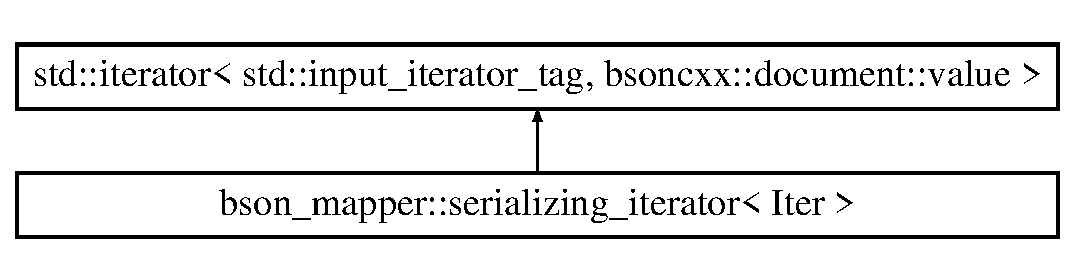
\includegraphics[height=2.000000cm]{classbson__mapper_1_1serializing__iterator}
\end{center}
\end{figure}


\subsection{Detailed Description}
\subsubsection*{template$<$class Iter$>$\\*
class bson\+\_\+mapper\+::serializing\+\_\+iterator$<$ Iter $>$}

An iterator that wraps another iterator of serializable objects, and yields B\+S\+ON document views corresponding to those documents. 

T\+O\+DO what to do if serialization fails? 

The documentation for this class was generated from the following file\+:\begin{DoxyCompactItemize}
\item 
src/bson\+\_\+mapper/mapping\+\_\+functions.\+hpp\end{DoxyCompactItemize}

\hypertarget{classbson__mapper_1_1UnderlyingBSONDataBase}{}\section{bson\+\_\+mapper\+:\+:Underlying\+B\+S\+O\+N\+Data\+Base Class Reference}
\label{classbson__mapper_1_1UnderlyingBSONDataBase}\index{bson\+\_\+mapper\+::\+Underlying\+B\+S\+O\+N\+Data\+Base@{bson\+\_\+mapper\+::\+Underlying\+B\+S\+O\+N\+Data\+Base}}


A base class that holds a shared\+\_\+ptr to the binary data for a B\+S\+ON document.  




{\ttfamily \#include $<$bson\+\_\+archiver.\+hpp$>$}



\subsection{Detailed Description}
A base class that holds a shared\+\_\+ptr to the binary data for a B\+S\+ON document. 

If a class you are serializing contains any of the bsoncxx view types (b\+\_\+utf8, b\+\_\+document, b\+\_\+array, b\+\_\+binary), you must have that class inherit this base so that the views don\textquotesingle{}t point to deallocated memory.

When using the \hyperlink{classbson__mapper_1_1BSONInputArchive}{B\+S\+O\+N\+Input\+Archive} to deserialize a class that inherits from this base, the data will be automatically loaded into this class using set\+Underlying\+B\+S\+O\+N\+Data(). 

The documentation for this class was generated from the following file\+:\begin{DoxyCompactItemize}
\item 
src/bson\+\_\+mapper/bson\+\_\+archiver.\+hpp\end{DoxyCompactItemize}

%--- End generated contents ---

% Index
\backmatter
\newpage
\phantomsection
\clearemptydoublepage
\addcontentsline{toc}{chapter}{Index}
\printindex

\end{document}
